\documentclass[11pt]{article}
\usepackage[T1]{fontenc}
\usepackage{lmodern}
\usepackage[margin=1in]{geometry}
\usepackage{amsmath,amssymb,amsthm,mathtools}
\usepackage{longtable,booktabs,array}
\usepackage{enumitem}
\usepackage{xcolor}
\usepackage{microtype}
\usepackage[hidelinks]{hyperref}
\usepackage{xurl}
\usepackage{graphicx}
\input{../paper/tex_fragments/figures/FIGURE_STYLE.tex}
\newcommand{\OPHPaperReleaseID}{r2069}
\newcommand{\OPHPaperReleaseDate}{November 19, 2026}
\newcommand{\OPHPaperReleaseBanner}{%
\begin{center}
\small\textbf{Paper release:} \texttt{\OPHPaperReleaseID}\quad\textbf{Released:} \OPHPaperReleaseDate
\end{center}
}
\newcommand{\PaperReleaseID}{\OPHPaperReleaseID}
\newcommand{\PaperReleaseDate}{\OPHPaperReleaseDate}
\newcommand{\PaperReleaseBanner}{%
\begin{center}
\small\textbf{Paper release:} \texttt{\PaperReleaseID}\quad\textbf{Released:} \PaperReleaseDate
\end{center}
}

% Section 2 states the basis, so the shared panel omits its basis paragraph.
\def\OPHOmitBasisPanel{}

\hypersetup{
  pdftitle={Observers Who Read Their Universe into Existence: Finite Consensus and the Reconstruction of Standard Physics},
  pdfauthor={Bernhard Mueller; Mario Poneder; Alexander Osika; Kai Xue; Ben Cassie; Peter Nguyen; Jinwook Kim; David Matscheko; Daniel Ari Friedman; Jonathan Hill; William T. Glynn; Maarten Antonie Visser; Kale Arnav Anirudha; Brieuc de La Fourni\`ere},
  pdfsubject={Finite observer-patch reconstruction in foundations of physics},
  pdfkeywords={foundations of physics, Observer Patch Holography, finite consensus, self-reference, quantum records, gauge structure, particle physics, Einstein field equation},
  pdflang={en-US}
}

\newtheorem{theorem}{Theorem}[section]
\newtheorem{proposition}[theorem]{Proposition}
\newtheorem{lemma}[theorem]{Lemma}
\newtheorem{corollary}[theorem]{Corollary}
\theoremstyle{definition}
\newtheorem{definition}[theorem]{Definition}
\theoremstyle{remark}
\newtheorem{boundary}[theorem]{Boundary}

\newcolumntype{L}[1]{>{\raggedright\arraybackslash}p{#1}}

\title{Observers Who Read Their Universe into Existence:\\
Finite Consensus and the Reconstruction of Standard Physics}

\author{%
\normalsize Bernhard Mueller\textsuperscript{1,*}\qquad
\normalsize Mario Poneder\qquad
\normalsize Alexander Osika\textsuperscript{2}\qquad
\normalsize Kai Xue\\[0.5em]
\normalsize Ben Cassie\qquad
\normalsize Peter Nguyen\qquad
\normalsize Jinwook Kim\textsuperscript{3}\qquad
\normalsize David Matscheko\\[0.5em]
\normalsize Daniel Ari Friedman\textsuperscript{4,5}\qquad
\normalsize Jonathan Hill\qquad
\normalsize William T. Glynn\qquad
\normalsize Maarten Antonie Visser\\[0.5em]
\normalsize Kale Arnav Anirudha\qquad
\normalsize Brieuc de La Fourni\`ere}
\date{\small\OPHPaperReleaseDate\quad\textperiodcentered\quad Paper release: \OPHPaperReleaseID}

\begin{document}
\maketitle

\begin{center}
\footnotesize
\textsuperscript{1}Pragma Research Inc.\quad
\textsuperscript{2}EtherWorks\quad
\textsuperscript{3}Oraclizer Labs\quad
\textsuperscript{4}Active Inference Institute\quad
\textsuperscript{5}FractiAI\\
\textsuperscript{*}Corresponding author:
\href{mailto:info@floatingpragma.ai}{\nolinkurl{info@floatingpragma.ai}}
\end{center}

\begin{abstract}
Observer Patch Holography formulates self-creation as a fixed-point
condition. Observers discover the laws of their history and build a
realization that reproduces it, including the builders. We implement
a finite computation on a spherical network of twelve-port cells.
From detector records alone the three spatial directions of a programmed
scalar wave can be recovered. With a material clock, the prescribed
refinement has a flat relativistic $3{+}1$-dimensional field limit on
bounded times and momentum bands.

Lean proofs give one public outcome for terminating, locally confluent
repairs from a fixed record. On a finite complex measurement algebra,
normalized probabilities additive on coexisting effects obey the Born
rule for a unique density matrix. Averaging local measurement outcomes
preserves the remote state. Quantum correlations attain the sharp CHSH
bound $2\sqrt{2}$. The cell has three independent slow responses. Twelve
independent port currents that close in a faithful, complete compact
algebra and implement cell rotations internally have the Standard Model
gauge Lie type.

Given the small-region area and matter-entropy relations, entropy
stationarity at fixed proper volume in every local frame yields the
Einstein equation up to a cosmological constant on a common Lorentzian
spacetime with conserved stress. In a separate semiclassical model,
two quantum fields source independently measured geometry under supplied
Einstein evolution. Deriving universal curvature and realizing the
closure condition on our observable history are tests of the full theory.
\end{abstract}




\vspace{0.5em}
\noindent\textbf{Keywords:} foundations of physics; Observer Patch Holography;
finite consensus; self-reference; executable model; quantum records;
emergent spacetime; gauge structure; particle physics; Einstein dynamics.

%=====================================================================
\section{Introduction}
\label{sec:intro}

A person at a computer works on a desktop. Windows stay where they were
put, files persist and the pointer glides across the screen. None of
these objects exists in the circuitry, which holds voltages in
registers. The desktop is the stable description that the interface
gives of those registers, and a user can learn reliable laws of the
desktop without ever seeing a transistor.

Observer Patch Holography (OPH) proposes that physics is a desktop of
this kind, seen by observers who are themselves part of the
computation. The hardware studied here is a sphere of small cells. Each
cell has twelve ports, neighbouring ports are joined by seams, and each
seam keeps a small private memory. One fixed local law acts on the
ports and seams. Nothing in this hardware is a position, a common clock
or a particle. Observers read their boundaries, write records, compare
records where they overlap and repair disagreements. What survives every
comparison is their public record, and space, time, fields and
particles are the descriptions observers fit to it. The thesis of this
paper is that these descriptions are the familiar ones: observers inside
the computation can describe their agreed records by a
three-dimensional space with relativistic time, stable particles, the
gauge structure of the Standard Model and gravity
(Figure~\ref{fig:desktop}).

\begin{figure}[!htb]
\centering
% Figure: the desktop picture of the flagship introduction. Hardware, agreed records and the effective description observers fit to them.
\begin{tikzpicture}[
  col/.style={oph box=#1, text width=4.2cm, align=flush left, inner sep=5pt, minimum height=40mm, anchor=north}]
\node[col=ophgrey] (hw) at (-5.85,0) {%
  {\footnotesize\bfseries The hardware}\\[4pt]
  {\scriptsize
  cells with twelve ports each\\
  seams with a private memory\\
  integer loads on the ports\\
  one local law, one coupling\\[4pt]
  no positions, no common clock\\
  and no particles}};
\node[col=ophnative] (rec) at (0,0) {%
  {\footnotesize\bfseries\color{ophnative} Agreed records}\\[4pt]
  {\scriptsize
  readings copied from both ends\\
  of a seam, kept when equal\\
  public records independent\\
  of the order of repairs\\
  Born weights, Tsirelson bound\\
  each observer's own count}};
\node[col=ophchecked] (desk) at (5.85,0) {%
  {\footnotesize\bfseries\color{ophchecked} The observers' desktop}\\[4pt]
  {\scriptsize
  three spatial directions\\
  flat $3{+}1$D wave equation (\S\ref{sec:three-directions})\\
  calibrated moving clocks lag\\
  stable particles (\S\ref{sec:observer-runs})\\
  Standard Model gauge structure\\ (\S\ref{sec:gauge})\\
  Einstein's equation (\S\ref{sec:einstein})}};
\draw[oph arrow=ophnative] ($(hw.east)+(0,-0.2)$)--($(rec.west)+(0,-0.2)$)
  node[midway, above, font=\scriptsize, text=ophnative, align=center] {read,\\compare,\\repair};
\draw[oph arrow=ophchecked] ($(rec.east)+(0,-0.2)$)--($(desk.west)+(0,-0.2)$)
  node[midway, above, font=\scriptsize, text=ophchecked, align=center] {fit a\\model};
\draw[oph arrow=ophgrey, dash pattern=on 2pt off 1.6pt, rounded corners=6pt]
  (desk.south) -- ++(0,-0.45) -| (hw.south)
  node[pos=0.25, below, font=\scriptsize, text=ophgrey] {closure: observers recover the specification of their hardware and build it (\S\ref{sec:strange-loop})};
\end{tikzpicture}

\caption{The desktop picture. The hardware is a finite computation on
registers. Observers inside it read, compare and repair records, and
what survives every comparison is public. The descriptions they fit to
their public records form their desktop; each entry names the section
that establishes it and states its premises there. The dashed arrow is
the closure hypothesis of Section~\ref{sec:strange-loop}.}
\label{fig:desktop}
\end{figure}

\paragraph{Space.} Imagine receiving the reports of eight stations with
their coordinates erased. Each station can launch a pulse, count local
clock events and report where the pulse was detected. Which stations are
neighbours? How many directions can a pulse travel? On the finite
computer studied here, the first round of detector counts answers both
questions. The eight stations have twelve links and three independent
binary coordinates. With the walk rule and a separately calibrated
material clock, these coordinates predict all twenty-four distributions
measured at three later clock readings. The largest absolute error in a
recorded probability is $0.001022$. Merging the stations along any one
recovered direction forces an error of at least $0.11377$ in the
corresponding population predictions. The positions just reconstructed
describe a scalar excitation carried by a programmed routing of the seam
interactions, and the routing is part of the apparatus. On bounded times
and momentum bands, refining the routing gives the Klein--Gordon
equation in flat $3{+}1$-dimensional spacetime
(Section~\ref{sec:three-directions}) \cite{ophmodel}.

\paragraph{Particles.} A desktop needs objects that keep their identity.
On the same hardware a local emitter writes two loads onto the two ends
of one seam, and then the law runs alone. A theorem bounds the
probability that the observers find no pair at a later first reading by
$40/(2\kappa-6)^2$ for every number of cells, where $\kappa>3$ is the one
coupling of the law. Observers read the pair on other seams than the one
it was written on, and nothing holds it together except the law.
The same law with its agreement energy removed loses the pair
(Section~\ref{sec:observer-runs}).

\paragraph{Gravity.} Gravity relates two independent measurements.
Matter changes the geometry that observers measure with clocks and
rulers, and the size of the change is fixed by the energy of that matter
measured with material probes. At fixed proper volume, positive
curvature shrinks the boundary area of a small ball. If entropy is
stationary, the area deficit balances the matter entropy inside. Ten
observers moving through one event, each measuring both sides on its own
shrinking balls, determine every component of Einstein's equation. A
modification of the executable model supplies all three measured inputs
on a material of clock pairs whose spherical pull and pair rule are part
of its declared law, and an independent light beam measures the focusing they predict
(Section~\ref{sec:einstein}).

\paragraph{Records and the machine itself.} Beneath these descriptions
lie the rules of records. Local repair that terminates and commutes on
overlaps leaves one public record whatever the order of repairs, and
completed records, represented on a finite quantum algebra, obey the Born
rule and the Tsirelson bound
(Section~\ref{sec:consensus}). An observer can also ask whether its
records reveal the machinery that made them. In a finite carrier
experiment, event logs and a specified set of probes determine the
twelve ports, their thirty internal seams and the local repair rule.
Running the recovered description reproduces the measured invariants
through two iterations. The closure hypothesis extends this kind of test
to an entire history. Its observers must recover a specification and
build a realization whose records and responses agree with the history
containing those observers, their discovery and their construction.
This is the physical meaning of self-creation proposed here
(Section~\ref{sec:strange-loop}) \cite{ophsim}.

\subsection{A short dictionary}
\label{sec:dictionary}

OPH uses a small number of terms in a precise sense. Their formal
definitions appear where they are first used, and their intuitive
meanings are collected here.

\begin{description}[leftmargin=1.2em,itemsep=1pt,parsep=0pt]
\item[Observer, or observer patch.] A finite bookkeeper inside the
computation. It holds some local state, reads the boundary it shares
with its neighbours, keeps records and uses them to choose its next
operation. It can be simple; the definition asks for no awareness. In
the executable model a cell, or a group of cells, is an observer and its
ports are its interfaces.
\item[Record.] The written outcome of a reading, which later events do
not erase. A record is \emph{public} when every authorized comparison
with neighbouring observers preserves it. No single observer owns it.
\item[Agreement.] Observers who share a boundary end with the same
record, whatever order their repairs took. Agreement concerns joint
probabilities and responses to interventions.
\item[Repair.] A local move that removes a disagreement between
neighbouring records while protecting what is recorded.
\item[Cell, port and seam.] The hardware. A cell, or carrier, has the
incidence of the icosahedron: twelve ports, thirty seams joining
neighbouring ports and twenty triangular faces. A port holds an integer
\emph{load}; a seam is the interface of two ports.
\item[Federation, or screen.] Cells joined port to port into a sphere.
It is the memory of the computation and no physical space.
\item[Seam memory and the echo.] Each seam keeps a private register. A
seam event writes the difference of its two loads, the \emph{contrast},
into it, gives the written label a phase and undoes the write. This is
the contrast-memory law. Its one coupling $\kappa$, the agreement
energy, lowers the energy of a seam whose two ports both hold a load.
\item[Interval Echo.] The main candidate law of the executable model:
the contrast-memory seam together with a clock that each observer patch
carries and verifies at every handoff.
\item[Own clock.] Each observer counts its own events. No common clock
exists, and observers relate their counts by comparing shared records.
\item[Emitter and reader.] Local instruments. An emitter writes a
prepared object onto a seam. A reader copies a yes-or-no answer from
both ends of a seam and admits it only when the two copies agree.
\item[Unrecovered seam, or collar.] A seam whose memory keeps a nonzero
contrast label while its ports show no contrast. It carries agreement
energy and no load.
\item[Desktop.] The effective description that observers give of their
agreed records: fields on a $3{+}1$-dimensional spacetime, particles and
forces. It is fixed by what observers can predict about their records
and says nothing about how the hardware stores them.
\item[Realization map.] The dictionary from finite records to laboratory
quantities such as positions, durations, currents and units
(Definition~\ref{def:physical-realization}).
\item[Candidate law.] A fully specified law on the fixed hardware. It is
tested through the records its observers produce. Changing the law, the
memory or the preparation defines a new candidate.
\item[Closure.] The hypothesis that a complete history contains the
discovery and the construction of its own specification,
$R(D(\mathfrak U))\cong\mathfrak U$ (Section~\ref{sec:strange-loop}).
\end{description}

\subsection{Mission}
\label{sec:mission}

The mission of OPH is a consistent and complete, formal and rigorous
theory of reality. Its proposed complete history has no external starting
point: it closes on itself. A successful theory must meet four conditions.
\begin{enumerate}
\item \textbf{Consistent.} Exhibit a history and its internal realization
that satisfy the closure condition, and verify the identification. An
explicit model witnesses the consistency of its stated assumptions.
\item \textbf{Explicit.} The complete recovered specification fixes its
consequences. Every design choice and calibration is declared; quantities
claimed as independent predictions are not inserted through those inputs.
\item \textbf{Complete}, in the sense Einstein, Podolsky and Rosen gave the
word \cite{epr1935}. Every element of physical reality has a counterpart in
the theory, and every measured quantity is derived.
\item \textbf{Correct.} Derived values agree with measurement, and new
predictions are frozen before they are tested.
\end{enumerate}
The mission ranges from the existence of an inhabited history and the
possibility of experience to the number of spatial directions, quantum
statistics, forces, particles, gravity and cosmology. This range specifies
what the proposed account must explain; it does not turn a finite model or a
conditional theorem into a derivation of every item. In particular, a
three-dimensional carrier response needs a physical position map, and an
operational observer needs an additional account before any claim about
phenomenal qualities follows. Table~\ref{tab:mission-coverage} gives these
distinctions alongside the physical results.

OPH does not claim to be the only theory with these properties. The four
conditions organize this paper. Consistency is tested through the closure
hypothesis and the executable model (Section~\ref{sec:strange-loop}) and
through the machine-checked results of Section~\ref{sec:verification}.
Specification and parameter ancestry are tested through the closure
coordinates of Section~\ref{sec:closure-principle}. Completeness is the ledger of realized
results and physical obligations in Section~\ref{sec:scoreboard}.
Correctness is decided by the frozen predictions and tests of
Section~\ref{sec:empirical}.

\subsection{Plan of the paper}
\label{sec:place}

Section~\ref{sec:strange-loop} states the closure hypothesis and how it
becomes a testable specification. Section~\ref{sec:architecture} gives
the hardware and its local law, and Section~\ref{sec:consensus} the
rules of public records, quantum probability and entropy. The four
sections after them carry the main results:
three-dimensional relativistic space (Section~\ref{sec:three-directions}),
stable particles (Section~\ref{sec:observer-runs}), forces and the
particle classes (Section~\ref{sec:gauge}) and gravity
(Section~\ref{sec:einstein}). Cosmology, the ledger of realized results,
the tests and the verification follow.

The program has four logically different levels. Closure proposes that an
inhabited history contains a recoverable account of its own operations. A
source specification states the carrier, observer access, repair, record and
state laws. Finite theorems and executable certificates determine what that
specification does. Physical realization asks whether one such source has
the observed fields, particles, clocks and responsive geometry. The
implications run in that order; Table~\ref{tab:program-status} states the
result at each level.

\begin{table}[htbp]
\centering\small
\caption{The OPH program and the status of its main implications.}
\label{tab:program-status}
\begin{tabular}{@{}L{0.18\linewidth}L{0.36\linewidth}L{0.38\linewidth}@{}}
\toprule
\textbf{Level} & \textbf{Result on its stated domain} & \textbf{Physical requirement}\\
\midrule
Closure & Finite consensus has an exact fixed-point packet theorem; a
universe-level self-recovering history is proposed & A specified history
and realization map satisfying the closure condition\\
Records and carrier & Canonical public records, conditional quantum
identities, finite entropy laws of repair and an exact rank-three slow
response & A common physical position, clock, energy and preparation map\\
Executable model & Interval Echo: three directions recovered from
anonymous detector counts and a flat $3{+}1$D wave limit of the programmed
scalar; the contrast-memory seam with its exact memory realization and a
binding theorem on every federation; bound objects that persist in the
agreed records; observer clocks whose closing rule is calibrated to the
proper-time forecast; twelve closed port currents & An
authenticated causal order with count and volume limits, one limiting speed
for bound objects, a complete current menu and one common measurement of
current and stress on a bound excitation\\
Gauge and matter & Complete-response premises force the Standard Model
Lie type; protected defects carry exactly the particle centre classes; port
phases give the global group & An interacting chiral field
with the observed species, quark flavours and mixing\\
Gravity and cosmology & Fixed-volume entropy balance and a calibrated
regional stress imply the Einstein equation on shrinking proper balls,
realized on a clock-pair material with a declared pull. Finite capacity
gives conditional
cosmological relations & The same source must supply conserved stress, responsive
geometry, vacuum, scales and prospective observational matches\\
\bottomrule
\end{tabular}
\end{table}

The finite results make OPH a concrete reconstruction program. Their
composition into the observed universe is a separate mathematical and
empirical claim. The specialist papers give the longer proofs, source
executions and failed attachments
\cite{ophparticles,ophGauge,ophEinstein,ophspine}.

Finite theorems, complete source executions and physical interpretations
answer different questions. We state each result's domain and supplied
inputs where it is used; the detailed claim classes and verification
methods are collected in Section~\ref{sec:verification}.

A result of the executable model is stated on records: the observer, the
record it holds and the probability the law gives for it. The state
vector, its levels, the evolution parameter and positions in a sequence of
events are tools of the calculation, and the text marks them as audit
where they appear. No common clock is assumed; each observer counts its
own events. The supplied parts of the construction are listed once, in
Section~\ref{sec:supplied}.

\begin{definition}[Physical realization map]
\label{def:physical-realization}
A physical realization map assigns finite public records, event data,
currents, modular generators, and scales to physical records, spacetime
events, laboratory currents, clocks, and units, preserving the algebraic
operations, overlap restrictions, causal order, normalizations, and
refinement relations consumed by the conclusion in question. A resemblance
of spectra, dimensions, or symmetry names is insufficient.
\end{definition}

The paper gives one mathematical representative of each step: the native
repair rule and its contrast-memory law, the consensus normalizer, the
spatial and gauge reductions,
the finite matter representation and the Einstein tensor implication. Its
status tables and prospective tests specify the physical conclusions.
The companion construction and component papers carry implementation
contracts and longer proofs
\cite{ophspine,ophrepo,ophnormalforms,opheventalgebra,ophconsensus,ophobservers,ophGauge,ophEinstein,ophMicrophysics,ophdesitter,ophyangmills,ophsim}.

%=====================================================================
\section{Closure: a universe that reads itself into existence}
\label{sec:strange-loop}

This section states the interpretation and acceptance criterion: closure, the internal-realization policy, the additional
state-selection and response-endogeneity principles, and the agreement
condition, then explains why closure is tested through an executable model.

\subsection{The closure hypothesis}

The universe is modeled as a timeless, closed, self-referential structure in which the description and the described system are one object.
Let $\mathfrak U$ be a complete inhabited history, let $D(\mathfrak U)$ be an
account of its architecture recoverable through completed records within it,
and let $R$ be an admissible realization of that account constructed inside
$\mathfrak U$. The closure condition is
\begin{equation}
R\bigl(D(\mathfrak U)\bigr)\;\cong\;\mathfrak U ,
\label{eq:closure-condition}
\end{equation}
where $\cong$ is agreement in the observable and interventional structure:
the records used to recover the description, and the responses of the
realization to every admitted intervention, fit the world from which the
account was recovered. Written as a fixed point of a
universe-level closure operator, the condition reads
$T(\mathfrak U)=\mathfrak U$. Observers infer the specification of their
world, build hardware within it, and run that hardware; its execution
realizes the same history, including its builders and their hardware. The
identification of the construction-side and inhabited-side readings is the
hypothesis. In this sense the structure reads itself into existence.

Within this hypothesis, no external computer runs the history and no
additional time exists in which the whole is played. Host runtime used to
check a model is part of our method of investigation, not an extra time
coordinate of the universe described by that model. Repair order is a partial order on commits, an observer
history is a chain of completed records, and that order is invariant under
strictly increasing regradings, so affine time and proper time require their
own calibration. Fixedness of the complete history permits changing states
within it: the equation concerns the whole history and identifies no last
instantaneous state with the universe.

A physical law is forced by a set of constraints if every admissible
realization obeys it. For example, on the finite
consensus branch the closure map is an affine idempotent. Its fixed
points are exactly the packets supported on consensus normal forms
\cite{ophconsensus}. This identifies a class of public records. To prove that closure
singles out our observable Universe, every admitted fixed history would
have to give the joint laws measured in our experiments, including those
withheld from the reconstruction. Two microscopically different
realizations could agree on all of those laws.

The finite reconstruction shows what can get lost in passing from
records to a specification. Event logs distinguish the local
icosahedral carrier from tetrahedral and octahedral controls. The
retained routing records nevertheless admit two port gluings with
different triangle counts and identical recorded bytes
(Section~\ref{sec:consensus}). A measurement sensitive to those gluings
would impose a further constraint. There is also a numerical closure
condition $N=\log M_0(\mathfrak U_N)$, where $N$ is the capacity budget
of the regulated observer system and $M_0$ is the correctable-code
capacity of its terminal public record. Base agreement, positivity and
the carrier bound leave that capacity underdetermined
\cite{ophobservers}. A universe-level existence claim requires a
specified history domain, an internal realization and a witness of
Eq.~\eqref{eq:closure-condition} on that domain.

\subsection{No outside}
\label{sec:no-outside}

A self-contained realization must account internally for its operations and
information access. This motivates a justification policy and two further
constitutive principles; it does not logically derive those principles.

\paragraph{Justification policy.} A premise is justified operationally when
observers recover it and the specification implementing it runs and
reproduces their measurements. The carrier, observer algebra, repair law and
closure coordinates must meet that test. Their specification can be
reconstructed from records or proposed as a design. In particular, using
a twelve-port carrier does not require a theorem that every possible
realization must have twelve ports. A construction choice needs no
uniqueness theorem unless uniqueness is claimed. Closure neither exempts a
candidate from empirical tests nor proves its antecedents jointly realizable.

\paragraph{State-selection principle.} On the declared feasible family,
reference, observer cover and positive weights, adopt the information
projection minimizing $\sum_pw_pD(\rho_p\Vert\tau_p)$. This is premise A3,
motivated by least-informative inference but separately adopted when used
as a physical selection law. The closure equation supplies no entropy
functional or reference; even its identity-map specialization fixes both
uniform and nonuniform states. Under A3, every minimizing local density has
the union of feasible supports, and a feasible failure witness $b>0$ gives
an explicit selected-probability floor \cite{ophEinstein}.

\paragraph{Response-endogeneity principle.} The complete-response branch
additionally requires each proper carrier recharting to be implemented by
the connected response group, up to a unitary centralizer acting trivially
on the response algebra. This is the endogeneity clause of A2, not a
consequence of internal implementation alone. For example, twelve diagonal
phase generators on $\mathbb C^{12}$ admit internal port permutations in
$\mathrm U(1)^{12}\rtimes A_5$. These permutations act nontrivially on the
abelian current algebra, whereas its inner automorphisms are trivial. This
closed operation system fails the stronger endogeneity premise; it shows
why that premise must be supplied. Theorem~\ref{thm:inner-action-closure}
uses it to select $\mathfrak u(1)\oplus\mathfrak{su}(2)\oplus\mathfrak{su}(3)$
under the stated complete-response hypotheses.

\subsection{Agreement and the meaning of ``our''}

The justification policy fixes the operational test. Agreement says what
counts as shared. Observers assign the same operational meaning to accepted
data on shared boundaries, naturally under every restriction, recharting and
refinement, and a record is public when it survives every authorized
comparison (Theorem~\ref{thm:confluence}). ``Our universe'' is the world
that this public record describes. Agreement in this sense is a definition
and an acceptance criterion: it requires interpretation maps fixed independently
of validation outcomes and preserving the declared joint and conditional
statistics, including quantum correlations. It does not require a
noncontextual table of outcomes for incompatible unperformed measurements.
Its content includes the joint probabilities and the response to changed
preparations. Once established by compatible records, these constraints
are public physical facts, and the equations that describe them assert no
additional material substrate beyond the specified process.
The theorem library calls the interpretation clause of this condition A2.
The basis reference distinguishes the closure hypothesis, agreement,
adopted selection/endogeneity principles and executable specification, with
the library's premise statements and their dictionary \cite{ophbasis}.

\subsection{An entry point without a starting point}

The exposition of this paper enters the loop at the executable
specification. That choice reflects where observers stand, holding records
and inferring, and it makes the account concrete. Closure states the internal
realization contract; the adopted principles and specification then carry
their own mathematical and empirical tests. The order of exposition is a logical entry point, not an event before
the universe or a privileged temporal beginning of the self-referential
loop. A pair of mutually determining
equations such as $x=(y+2)/2$, $y=(x+2)/2$ fixes $x=y=2$ with no first value
from which the other is manufactured; a calculator may approach the pair by
iteration and someone may find it on a particular day, and neither belongs
to the reason the answer is two.

The closure equation relates parts of one timeless object; it posits no
backward signal in an external time coordinate. Observers recover the specification and later construct
it in their own record order, and both stages belong to the same fixed
point. In the terminating consensus theorems, repair descent supplies a
well-founded order on the admitted updates for proving termination and
comparing schedules; it is neither an observer's
experienced time nor a universe-level clock.

The observer who infers a law and the hardware that realizes it both
belong to the candidate history. If several specified closures satisfy
the same tests, the results warrant that observational class without a
uniqueness claim.

\subsection{From closure to a testable specification}
\label{sec:closure-to-model}

The executable observer gives the condition its finite meaning. A
realization differs from a description because it carries the described
dependencies under intervention: for a described update $\tau_a$, realized operation $F_a$ and fixed readout $p$, the one-step condition $p(F_a(s))=\tau_a(p(s))$ extends by induction to every finite admitted sequence. A playback can match every frame of one history and fail
this test as soon as a retained state is changed. The controls of
Section~\ref{sec:observer-runs} apply this test to the executable model:
a changed preparation and a changed law, run through the same emitter and
reader, change the agreed records.

Closure alone does not imply that a particular carrier, record law or initial
state yields Standard Model physics. The executable-model hypothesis is the
stronger claim that one simple, fully specified law does, and it is the form
in which closure can fail. Its carrier architecture, refinement and
composition, record instruments, memory law, scheduler, preparations and
available controls are stated before testing. A failed specified law
rejects that law and its tested interpretation; it reaches the wider
proposal only when the rejected choice is proved necessary and exclusive.
Changing the law, memory, state or decoder defines a new candidate.

The main candidate law of the executable model is Interval Echo. It runs
the contrast-memory law of Section~\ref{sec:contrast-memory}, the law of the
reference candidate A-contrast-memory-spherical-v1, and adds a clock that
each observer patch carries. On its programmed scalar instrument,
observers recover three directions from anonymous detector counts, and
the refinement has a flat $3{+}1$-dimensional wave limit
(Sections~\ref{sec:blind-chart} and~\ref{sec:scalar-limit}). The shared
seam interaction reproduces particle stability: bound objects persist in
free evolution, read on the agreed records of the observers, and the same
law with the agreement energy removed loses them
(Section~\ref{sec:particle-stability}). The clock of Interval Echo
implements the calibrated reunion rate on a supplied relay
(Section~\ref{sec:travelling-clock}), and a modification with published
clock records realizes the Einstein premises on pressureless matter
whose spherical pull and pair rule are declared
(Section~\ref{sec:einstein-dust}). Under a further candidate law on the same carrier an object on four seams is kept
for every interval and carries a prepared clock, read from counts in units
of the observer's own reference \cite{ophmodel}. The construction supplies
no selection of its couplings, and its calibrations are declared. The
physical obligations of Section~\ref{sec:scoreboard} are the
tests the candidates have to pass on one process.

\subsection{Specification and theorem premises}
\label{sec:specification-premises}

The architecture, record instruments, memory law, scheduler, preparation
services and allowed interventions form a declared specification. Observers
may infer or design these ingredients; mathematics determines their
consequences, and comparison determines whether the resulting process
matches observed physics. Declaring a primitive fixes the model under
study. Its consequences require proofs, and its physical adequacy
requires tests; a specified input must remain distinguishable from a
consequence derived from other inputs. The carrier, memory and control laws need not be uniquely
selected by closure to be legitimate inputs. Their implementation and
resource use must, however, belong to the process being studied.

Three premise families recur. A1 specifies the carrier, federation and
response structure. A2 adds agreement on shared records and inner
implementation of the complete response algebra. A3 adopts a
least-informative state-selection principle on the stated feasible family.
Closure alone proves neither the entropy minimizer nor the inner
implementation assumption. Later theorems state which of these inputs
they use and which additional hypotheses their conclusions require.

Quantum executions below use finite-dimensional complex Hilbert spaces,
positive normalized density operators and completely positive instruments
whose complete effects sum to the identity. These are explicit quantum
premises, not consequences of classical normal-form uniqueness. A faithful
reference is a strictly positive density operator $\rho>0$; its modular
flow is $\sigma_s(A)=\rho^{is}A\rho^{-is}$. The dimensionless parameter $s$
requires a separate implemented calibration before it is read as duration.

The physical interpretation also fixes a domain: one prepared history,
a family of interventions, or every allowed input state. These are
inequivalent requirements. Complete quantum instruments must retain the
reference systems and all outcomes needed for the chosen domain; a record
history need not assign simultaneous values to unperformed incompatible
measurements. Likewise, a stationary probability law, an instantaneous
repair fixed point and the closure of an entire history are distinct.
Host runtime, repair counts, modular parameters and measured duration are
related only by an implemented clock calibration. The operational observer
below is defined by access and record interfaces, without an additional
claim about consciousness.

%=====================================================================
\section{The hardware: cells, seams and the local law}
\label{sec:architecture}

The observer-service theorems use an operational observer and a twelve-port
carrier with its specified repair law. These define the service domain.
The executable model runs the same seam event without committing it:
Section~\ref{sec:contrast-memory} states the seam law of its candidates and
Section~\ref{sec:observer-runs} their operation.

\subsection{Patches, records and repair}

\begin{definition}[Observer patch]
An observer patch is a finite object with local state, an observable boundary
map, durable records, readback, and a set of authorized repair moves. A
patch sees a fragment of the world: its own state and the boundary data of
its authorized overlaps.
\end{definition}

\begin{definition}[Overlap and repair]
For patches $x_i$, $x_j$ with an authorized overlap $e=(i,j)$, both induced
boundary records must agree for the pair to hold public data. A repair move
changes local state while preserving protected readout. A configuration is a
normal form when no authorized repair applies.
\end{definition}

An observer in this sense is defined by its access and record interfaces.
It reads, writes and retains records, and it uses retained records to choose
its next operation. Nothing in the definition refers to a background space,
a global clock or a pre-assigned list of particles. Those enter later as
readouts that observers can share.

\subsection{The twelve-port carrier}

Each local carrier has twelve boundary ports, thirty seams and twenty
oriented triangular faces. The incidence has a selection theorem that uses no
topological template, Euler count, group action or preassigned port count.

\begin{theorem}[Icosahedral incidence from optimal readout]
\label{thm:carrier-selector}
In a real three-dimensional response space, let unit vectors $u_i$ read symmetric
operators through $\operatorname{tr}(P_iX)$, $P_i=u_iu_i^{\mathsf T}$, with positive
weights $\sum_iw_i=1$, and put $M=\sum_iw_i|P_i\rangle\langle P_i|$. Informational
completeness requires at least six distinct channels, and every choice obeys
$\lambda_{\min}(M)\leq2/15$. With six channels, equality holds exactly for equal weights
and the six icosahedral axes, up to an orthogonal frame. Exposing both signs gives twelve
ports, positive overlap gives degree five and thirty edges, and the three-cliques give
twenty faces. A deficit of at most $10^{-7}$ forces the same incidence, without forcing
exact angles.
\end{theorem}

\begin{proof}
$\operatorname{Sym}(3)$ has dimension six and each term of $M$ has rank one. Each
$P_i-I/3$ has squared norm $2/3$, so the trace-free compression of $M$ has trace $2/3$ on
five dimensions, which gives the bound. Equality forces $M(X)=(2X+\operatorname{tr}(X)I)/15$.
At six channels the matrix $F$ with columns $\sqrt{w_i}P_i$ is invertible and
$F^{\mathsf T}M^{-1}F=I$: its diagonal gives $w_i=1/6$ and its off-diagonal gives
$(u_i\cdot u_j)^2=1/5$. The Gram matrix $I+S/\sqrt5$ then has a sign matrix with $S^2=5I$,
whose unique switching class fixes the geometry \cite{ophMicrophysics}.
\end{proof}

The response dimension, the quadratic readout, both objectives, inverse ports and
positive-overlap edges are premises, and a physical metric requires operational
reconstruction. Carriers federate through typed seam
algebras and coherent triple overlaps into a nerve with a degree-one bridge
to an oriented sphere.
Native current records recover the local Gram; executed cross-carrier
routing uses supplied cell centres and tangent frames. A1 in the theorem
library declares this carrier, federation and response layer.

Two exact features of the carrier enter later constructions. First, the
proper rotation group of the icosahedral packet is the alternating group
$A_{5}$, with sixty rotations acting on the twelve ports, and the real
port-coefficient space decomposes without multiplicity as
\begin{equation}
P_{12}\;\cong_{A_5}\;\mathbf 1\oplus\mathbf 3\oplus\mathbf 3'\oplus\mathbf 5 .
\label{eq:bands}
\end{equation}
On the six-dimensional golden sector the spectral projectors have entries in
$\tfrac1{20}\mathbb Z[\varphi]$, $\varphi=(1+\sqrt5)/2$, each is the
entrywise Galois conjugate of the other, and both triplets are irreducible
real representations of real type; the projectors, characters and
irreducibility certificates are machine-checked
\cite{serre1977,ophrepo}. Second, record keeping is integer valued: a write
appends $+1$, a retraction appends $-1$, and readback sums atomic events per
port. A conservative repair transfers one unit across a seam whenever the
oriented mismatch has magnitude at least two. With $V(x)=\sum_ix_i^{2}$, each such repair strictly decreases $V$ by $2(d-1)$ for mismatch $d\ge 2$,
so repair terminates. The native repair law of
Section~\ref{sec:native-repair} also moves load to the floor and ceiling of
the endpoint mean, but at difference one it waits or swaps by its coin, so
the native process keeps moving while its quadratic cost stays fixed.

\subsection{The native repair law}
\label{sec:native-repair}

\begin{figure}[!htb]
\centering
\input{../paper/tex_fragments/figures/FIG_CARRIER_SEAM_RULE.tex}
\caption{The twelve-port carrier and its native repair. Left: the icosahedral incidence of the twelve ports, with thirty seams and twenty faces, in an orthographic view with back edges dashed; the filled ports carry a binary load of total two, and the drawn seam $(a,b)$ has $d=1$. Right: the seam rule for every mismatch the total-two carrier admits.}
\label{fig:carrier}
\end{figure}

The seam event acts on integer loads. One carrier with twelve nonnegative
integer loads of total two has $78$ configurations, and the $66$ binary
configurations form an invariant shell. For an oriented seam $(a,b)$ and a
fair placement coin $c\in\{0,1\}$ (Figure~\ref{fig:carrier}), the native repair law moves
\begin{equation}
d=x_a-x_b,\qquad
j=\tfrac12\bigl[d-(2c-1)(|d|\bmod 2)\bigr],\qquad
y=x+j\,(e_b-e_a),
\label{eq:native-repair}
\end{equation}
so load is conserved and the signed current $j$ is the native observation.
Conservation, one-step balance, a tie-break that reads no load and endpoint
symmetry characterize this rule; on the total-two carrier they fix only the
tie-break coin.

The event can be completed in two ways. Committed repair reads the event
into a public record. Its quantum version is a record law, and seam
locality, the classical law and the declared local number-phase and
endpoint-swap covariance, a local phase symmetry of the repair channel, leave a convex
family of them, each a table of five coherence multipliers
\cite{ophrecordlaws}. Every member has the load update
\eqref{eq:native-repair}. The unread channels have a source-independent
spectral gap $(5-\sqrt5)/60$ on the binary shell. Every admissible coherence
table has the uniform binary state as its unique stationary state, and the
rank-three load readings of Theorem~\ref{thm:rank-three} attain the slow
rate \cite{ophrecordlaws,ophmixing}. Section~\ref{sec:thermodynamics} gives
the entropy laws of committed repair. A committed record attenuates
coherence, so it cannot be unitary conjugation on this carrier.

The second completion keeps the event private and coherent. It is the seam
interaction of Interval Echo, the main candidate law of the executable model,
defined in the next subsection.

\subsection{The contrast-memory law}
\label{sec:contrast-memory}

The contrast-memory law keeps the carrier and the seam event and completes
the event by an echo. It is the law of the reference candidate
A-contrast-memory-spherical-v1 and, at $\kappa=8$, the seam interaction of
the main candidate, Interval Echo. A cell is one twelve-port carrier. Every port
holds a load in $\{0,1,2\}$; write $n_v$ for the load of port $v$ as an
operator. Every seam carries a private memory of eleven states: one blank
state and ten labels $(c,d)$, with the coin $c\in\{0,1\}$ and the contrast
$d\in\{-2,\dots,2\}$, the difference of the two loads of the seam. The
memory is coherent working memory of the seam, shared by its two ports.
It is no public record.

For loads $(a,b)$ on a seam put $s=a+b$ and $p=s\bmod2$. The seam event
\eqref{eq:native-repair} has the two outputs
\begin{equation}
 y_c=\bigl(\lfloor s/2\rfloor+cp,\ \lfloor s/2\rfloor+(1-c)p\bigr),
 \qquad c\in\{0,1\},
\label{eq:seam-outputs}
\end{equation}
and the contrast write stores coin and contrast beside them:
\begin{equation}
 W|a,b\rangle=\frac1{\sqrt2}\sum_{c=0}^{1}|c,a-b\rangle\otimes|y_c\rangle .
\label{eq:contrast-write}
\end{equation}
The write $W$ is an isometry on all nine local inputs. The local space has
dimension $99$, nine load states times eleven memory states, and splits
into the sector of blank memory and the sector of labels. On it
\begin{equation}
 U=\begin{pmatrix}0&W^{*}\\ W&I-WW^{*}\end{pmatrix}
\label{eq:echo-unitary}
\end{equation}
is a Hermitian unitary on every state, dirty memory included. On the
labels put $R|c,d\rangle=|c,-d\rangle$ and $D|c,d\rangle=d\,|c,d\rangle$.
The memory generator and the local term of the law are
\begin{equation}
 G_\kappa=0_{\rm blank}\oplus\Bigl[\frac{I-R}{2}+\kappa D^2\Bigr]\otimes I,
 \qquad h_\kappa=U\,G_\kappa\,U^{*}.
\label{eq:echo-term}
\end{equation}
The term $h_\kappa$ is an echo: the write, a phase on the written label,
and the reverse write (Figure~\ref{fig:echo}). The part $(I-R)/2$, with
$R$ the reversal of the retained contrast, gives the exchange, and the
part $\kappa D^2$ is a phase proportional to the square of the retained
contrast. The coupling $\kappa$ is one dimensionless number, the agreement
energy in units of the exchange.

\begin{figure}[!htb]
\centering
% Figure: the echo of the contrast-memory law and the two fates of the label of a seam event.
\begin{tikzpicture}[
  st/.style={oph box=ophnative, text width=3.1cm, minimum height=13mm},
  op/.style={font=\scriptsize, align=center}]
\node[st] (in) at (0,0) {loads $(a,b)$ on a seam\\[1pt]{\scriptsize memory blank}};
\node[st, text width=4.1cm] (mid) at (5.6,0) {outputs $y_c$ of the event\\[1pt]{\scriptsize memory holds $(c,d)$, $d=a-b$}};
\node[st] (out) at (11.2,0) {loads on the seam\\[1pt]{\scriptsize memory blank}};
\draw[oph arrow=ophnative] (in)--(mid) node[midway, above, op, text=ophnative] {write};
\draw[oph arrow=ophnative] (mid)--(out) node[midway, above, op, text=ophnative] {reverse\\write};
\node[op, text=ophnative, anchor=south] at ($(mid.north)+(0,0.12)$) {phase $\tfrac12(I-R)+\kappa D^2$ on the label};
\node[oph box=ophdeclared, text width=4.1cm, minimum height=11mm] (rec) at (5.6,-2.2) {public record of $(c,d)$\\[1pt]{\scriptsize committed repair, law E}};
\draw[oph arrow=ophdeclared, dash pattern=on 2pt off 1.5pt] (mid)--(rec) node[midway, right, op, text=ophdeclared] {read};
\node[oph label, anchor=west] at ($(in.west)+(0,-1.55)$) {the echo: the label stays private};
\node[oph label, anchor=west] at ($(in.west)+(0,-1.95)$) {and the event stays coherent};
\begin{scope}[shift={(8.6,-2.05)}]
\node[oph label, anchor=west] at (-0.2,0.62) {cost of two loads in $C$};
\draw[ophnative, line width=1.2pt] (0,0)--(0.6,0);
\fill[ophnative] (0,0) circle (1.3mm);
\fill[ophnative] (0.6,0) circle (1.3mm);
\node[oph label] at (0.3,-0.45) {pair $10$};
\draw[ophgrey!60, line width=0.5pt] (1.6,0)--(2.8,0);
\fill[ophnative] (1.6,0) circle (1.3mm);
\draw[ophgrey, fill=white, line width=0.5pt] (2.2,0) circle (1.3mm);
\fill[ophnative] (2.8,0) circle (1.3mm);
\node[oph label] at (2.2,-0.45) {separate $12$};
\node[circle, fill=ophnative, text=white, inner sep=0pt, minimum size=3.4mm, font=\scriptsize\bfseries] at (3.9,0) {2};
\node[oph label] at (3.9,-0.45) {doubled $24$};
\end{scope}
\end{tikzpicture}

\caption{The echo of the contrast-memory law. The write stores the coin and the contrast of a seam event in the private memory of the seam, the label acquires a phase, and the write is reversed. Reading the label into a public record at the middle step is committed repair. Lower right: the cost in $C$ of two loads on one seam, on separate ports and on one port.}
\label{fig:echo}
\end{figure}

\begin{proposition}[Exact reduction on blank memory]
\label{prop:echo-reduction}
Let $J$ embed the load states of a seam with blank memory. For every real
$\kappa$,
\begin{equation}
 h_\kappa J=J\Bigl[\frac{I-\mathrm{SWAP}}{2}+\kappa\,(n_a-n_b)^2\Bigr],
\label{eq:echo-reduction}
\end{equation}
where $\mathrm{SWAP}$ exchanges the two loads of the seam. Every local
term preserves the blank memory, so the sum of the terms of overlapping
seams preserves the product of blank memories.
\end{proposition}

\begin{proof}
The outputs \eqref{eq:seam-outputs} depend on $a$ and $b$ through their
sum alone, so $(R\otimes I)W=W\,\mathrm{SWAP}$ and
$(D^2\otimes I)W=W(n_a-n_b)^2$. Write $M$ for the bracket of
\eqref{eq:echo-reduction}. Since $UJ$ is the write into the label sector
and $U^{*}=U$, these identities give $G_\kappa UJ=UJM$, and $U^2=I$ gives
$h_\kappa J=UG_\kappa UJ=JM$. A symbolic computation confirms the identity
on all $99$ local states \cite{ophmodel}.
\end{proof}

In a federation, cells are joined by external seams that form a partial
matching on ports. Every cell has three external ports, so a port has
$d_v=5$ or $d_v=6$ seams. A port with five seams carries one private
reference register held at zero, on which the $D^2$ part of the generator
acts alone, so every port counts six. Summing \eqref{eq:echo-reduction}
over the seams $e=(a,b)$ gives the law on the loads,
\begin{align}
 H_\kappa&=\frac12\sum_e(I-\mathrm{SWAP}_e)+\kappa\,C,
\label{eq:contrast-law}\\
 C&=\sum_e(n_a-n_b)^2+\sum_v(6-d_v)\,n_v^2
  =6\sum_vn_v^2-2\sum_en_an_b .
\label{eq:contrast-cost}
\end{align}
An agreed seam, one whose two ports both hold a load, lowers $C$ by two.
A pair of loads on the two ends of one seam costs $10$ in $C$, two
separate loads cost $12$ and a doubled load costs $24$. The law conserves
the number of loads and the multiset of port loads.

For one load $H_\kappa=L/2+6\kappa$, with $L$ the graph Laplacian. On one
cell the levels of $L/2$ are $0$ on the uniform mode, $(5-\sqrt5)/2$ three
times, $3$ five times and $(5+\sqrt5)/2$ three times. The first triplet is
the slow band of Theorem~\ref{thm:rank-three}: on one load the exchange
part is $L/2=30\,(I-M)$, with $M$ the repair mean of that theorem and
thirty the number of seams.

The two completions share the seam event and differ in the fate of its
label. Committed repair reads the label into a public record: reading
$(c,d)$ after the write \eqref{eq:contrast-write} records the coin, the
current and the parity $p_e$ of the seam's total load, since
$d=2j+(2c-1)p_e$. The echo reads nothing. It reverses the
write, the label stays in the private memory of the seam, and the event
stays coherent. On binary loads the exchange term
$(I-\mathrm{SWAP}_e)/2$ equals $I-P_e$, where $P_e=(I+\mathrm{SWAP}_e)/2$
is the unread population channel of committed repair
(Section~\ref{sec:thermodynamics}). Committed repair applies $P_e$ to
populations; the law generates the same exchange on amplitudes.

On loads $0$ and $1$ the seam term is the ferromagnetic XXZ interaction
\begin{equation}
 h_e=\frac{(1+2\kappa)(I-Z_aZ_b)-X_aX_b-Y_aY_b}{4},
\label{eq:xxz}
\end{equation}
and the binding of Section~\ref{sec:binding} is of the droplet kind known
from that literature \cite{nachtergaelestarr2001,fischbacherstolz2018}.
The construction claims no interaction of its own invention. Its content
is the memory realization, the constants on this carrier and the tests on
records.

%=====================================================================
\section{Public records and the quantum rules}
\label{sec:consensus}

The repair mathematics establishes when local agreement reaches global
consistency and when nonzero cycle holonomy leaves a residue that local
repair cannot remove.
Two observers who share a boundary can disagree about what it shows. If
repair stopped in different places depending on who acted first, the
boundary would carry no fact of the matter. If it always stops in the same
place, the final record is a public fact that no single observer owns. This
section states when the second case holds, and then shows that completed
records satisfy the familiar quantum identities on the declared complex
algebra and state domain below.

A completed finite configuration $x$ is a fixed point of the named
repair-and-agreement map,
\[
\mathcal R_{\mathrm{cons}}(x)=x .
\]
This map is
distinct from the universe-level closure operator of
Section~\ref{sec:strange-loop}. Fixed-point existence, observable
determination and schedule independence are separate questions, and the
following results isolate them \cite{ophnormalforms,ophconsensus}.

\subsection{Observable normal forms}

\begin{definition}[Observable quotient system]
An observable quotient system is a tuple $\mathfrak S=(Q,C,\mathcal B,B)$,
where $Q$ is a set of configurations, $C\subseteq Q$ is the consistent
subset, $\mathcal B$ is a set of protected records, and $B:Q\to\mathcal B$
is the record map. For $b\in\mathcal B$, write $C_b=C\cap B^{-1}(b)$.
\end{definition}

The fiber $C_b$ is unrealizable, reconstructing, or ambiguous according as
its cardinality is zero, one, or greater than one. This trichotomy avoids
assigning a state to a record that has either no consistent extension or
several observationally indistinguishable extensions.

\begin{theorem}[Canonical observable normalizer]
\label{thm:observable-normalizer}
The following statements are equivalent:
\begin{enumerate}[label=(\roman*),leftmargin=1.6em]
\item $B|_C$ is injective;
\item there is a unique map $\mathcal N:Q\to C\sqcup\{\bot\}$ that preserves $B$ on
its $C$-valued outputs, fixes every point of $C$, is constant on each
$B$-fiber, and returns $\bot$ exactly on fibers with no consistent extension;
\end{enumerate}
If $B(Q)\subseteq B(C)$, the map is a total idempotent retraction $Q\to C$.
\end{theorem}

\begin{proof}
Injectivity makes every nonempty $C_b$ a singleton, which defines $\mathcal N$ and forces all its properties fiber by fiber. Conversely, if $c,c'\in C$ have $B(c)=B(c')$, the fixed-point and fiber clauses give $c=\mathcal N(c)=\mathcal N(c')=c'$.
\end{proof}

The normalizer is defined by observable fibers, independently of any repair
schedule; a repair relation implements it when the relation preserves $B$,
reaches the consistent set and satisfies a liveness condition. Approximate
versions control the normalizer where exactness fails, through an optimal
two-output distance bound and summable naturality defects along refinement
towers. Canonicity carries no promise of cheapness: for succinct Boolean
boundary systems, deciding whether a protected record has a consistent
extension is NP-complete, and deciding injectivity of the record map is
coNP-complete \cite{ophnormalforms}.

For the canonical single-site repair, every adaptive run is eventually
constant because each nonstuttering attempt strictly lowers the mismatch
count; pathwise weak fairness makes the stable state a normal form, and
completeness with confluence sends every weak-fair run to the same public
fixed point. These results select no scheduler and provide no stochastic hitting law, rate, physical clock, or refinement theorem.
Attempts obey a sharp capacity law. A scheduler can delay the first genuine repair for any prescribed number of attempts. When every reducible record sees a genuine change among the next $q+1$ attempts, a bounded-waste upper horizon of $(q+1)$ times the initial mismatch count holds, and an independent-defect family attains the work-conserving case exactly at $q=0$.
The input-independent compiler produces a fixed federation with immutable input ports;
genuine node repairs decrease a dependency rank, and pathwise weak fairness
gives stable consensus and the correct output.
Emission-order round robin finishes within its first $n$ attempts, and the single-consumer structure bounds every accepted path by $n(n+1)/2$, with an emitted family attaining $\Theta(n^2)$.
General well-formed circuits instead admit $2^n-1$ accepted steps, attained by a fanout chain, where $n$ counts the emitted nodes.
These statements concern canonical node repairs: the weak patch-frame relation can stutter fairly forever, and no physical scheduler, clock, energy or hardware cost follows from these operation counts \cite{ophnormalforms,ophconsensus}.

\subsection{Public records from local repair}

For a prepared batch of support-closed transactions, join $\tau$ and $\sigma$
in the conflict graph when
$W_\tau\cap(R_\sigma\cup W_\sigma)\ne\varnothing$ or
$W_\sigma\cap(R_\tau\cup W_\tau)\ne\varnothing$, and iterate to a fixed
point: compute semantic support inside every aggregate, rebuild the conflict
graph on the expanded read and write sets, merge every connected component,
and repeat until the partition and all aggregate supports are unchanged.

\begin{proposition}[Transactional local diamond]
\label{prop:transactional-diamond}
Let an accepted repair be an aggregate transaction with read set $R_\tau$,
write set $W_\tau$, a read snapshot, and a snapshot-determined payload.
Assume:
\begin{enumerate}[label=(\roman*),leftmargin=1.6em]
\item every read set contains the semantic dependency closure of its write
set, and every affected acceptance functional is revalidated at commit;
\item the terminal closure above exists, and each of its connected conflict
components has one coherent canonical aggregate payload;
\item a prepared component whose snapshot remains valid survives commits of
independent components; and
\item accepted commits preserve the protected record and strictly decrease
the integer descent functional.
\end{enumerate}
Then every one-step quotient peak $t\longleftarrow s\longrightarrow u$ has a
quotient state $v$ with $t\longrightarrow v\longleftarrow u$.
\end{proposition}

\begin{proof}
Two different first steps cannot originate in one conflict component, since
that component has a unique aggregate payload, so they originate in distinct
components of the terminal closure. Rebuilding the graph after every
aggregate support expansion makes their final read and write sets disjoint,
so neither commit changes the other's read snapshot, and semantic dependency
closure ensures neither changes an acceptance functional consumed by the
other. Revalidation and the surviving component rule make both second
commits legal, and with snapshot-determined payloads and disjoint writes the
two application orders agree; protected-record preservation carries the
equality to the physical quotient.
\end{proof}

\begin{theorem}[Consensus normal form]
\label{thm:confluence}
Suppose the accepted repair relation satisfies the hypotheses of Proposition~\ref{prop:transactional-diamond}, so that it has the one-step diamond property, strictly decreases the quadratic descent functional $V$ of Section~\ref{sec:architecture}, and is repair complete, meaning that its normal forms are exactly the consistent states. Every maximal asynchronous
repair schedule from one initial state then terminates at the same consistent
quotient normal form. The induced global repair map is idempotent, fixes
consistent states, and preserves the protected record.
\end{theorem}

\begin{proof}
Quadratic descent makes the accepted relation terminating.
Proposition~\ref{prop:transactional-diamond} makes it locally confluent, so
Newman's lemma \cite{newman42} makes it confluent. A terminating confluent
relation has a unique normal form below each source, and repair completeness
puts that normal form in the consistent set. Applying the normalizer a second
time does nothing, and protected-record preservation holds along every
accepted edge.
\end{proof}

Atomic commits, disjoint write sets, or termination alone do not imply the
local diamond; countermodels omitting semantic dependency closure, canonical
aggregation or the surviving component rule are retained with the finite
receipt. This is the precise sense in which a public fact is what survives
every authorized comparison: the public object is the protected quotient
record, independent of the order in which observers repaired.

Repair also has a residue that it cannot remove. On a fixed graph with
positive mismatch weights and fixed edge offsets, nonzero cycle holonomy
forces a strictly positive minimum mismatch, and no repair of the vertex
assignments eliminates it while the offsets are fixed \cite{ophconsensus}.
The protected defects that this frustration leaves behind are the particle
families of Section~\ref{sec:defect-families}.

The law runs at scale. The public run uses the level-six cell rung of the
geodesic icosahedral refinement tower: $81{,}920$ exact twelve-port carriers
with one declared gluing of ports to neighboring cells, $2{,}580{,}480$
seams in all, and the seam-mean retraction as repair primitive. Sixteen
shuffled schedules from one seeded load terminate at the balanced class with
no accepted move raising $V$, and all sixteen return one quotient hash equal to the component multiset fixed by the initial totals.
A standalone verifier that imports no simulator code rebuilds the component
multisets from the primitive arrays, replays one schedule from its seed and
recomputes every hash \cite{ophsim}. The level-ten rung, with $20{,}971{,}520$ carriers and $660{,}602{,}880$ seams,
terminates all sixteen schedules at the balanced class in $84$ to $100$ sweeps
with one quotient hash fixed by the loads. The excess-energy contraction per sweep lies between $0.81$ and $0.83$ across rungs five to nine, and these finite readings prove no all-size mixing or termination-time bound. Stationary continuation adds a
constructive fluctuation result: for fair integer repair on a connected
weighted graph with independent edge clocks of total rate one the fixed-occupancy law is reversible, centered loads have lagged covariance $\kappa e^{-|t|L_G/2}\Pi$ in the edge-clock time $t$, with $L_G$ the weighted graph Laplacian,
$\kappa=r(p-r)/(p(p-1))$ for $r$ raised occupancies on $p$ ports and $\Pi$ the
projection off constants, and fixed linear readouts obey a martingale central
limit theorem \cite{ophMicrophysics}.

The same records let observers recover the specification itself.
At carrier scale, recovery from event logs under the declared probe and
operation grammar returns the twelve ports, thirty seams, inverse pairing,
automorphism and rotation groups of orders $120$ and $60$, mean rule,
schedule, rank-three Gram and Lie split $1+3+8$.
Re-instantiation preserves the invariant vector for two iterations, and
tetrahedral and octahedral controls recover their distinct specifications
\cite{ophsim}. Complete federation gluing is not identified by the retained routing logs: within the declared port-gluing interface a two-edge switch preserves every carrier degree, occupied port and source traversal while changing the carrier graph's triangle count from $14{,}000$ to $13{,}990$, and native executions reproduce identical bytes for both.
The alternative is not asserted to belong to the canonical geometric family.
Full-gluing recovery requires further observations or a justified
restriction of the candidate class.

\subsection{Completed records and quantum identities}
\label{sec:quantum}

Once a compare, write and verify slice has completed, its accessible events
are represented in a finite-dimensional complex $C^*$-algebra with a
positive normalized state and completely positive instruments. This
algebra-state representation is an explicit input; the consensus theorem
identifies which record is public and does not by itself select complex
quantum theory over every alternative probability model.

\begin{theorem}[Finite public-record identities]
\label{thm:born}
Let $P_E$ be the projector of a completed public event $E$ and $\rho$ the
normalized state of the completed record surface. The event weight and
nonzero-weight update
\begin{equation}
\Pr(E)=\operatorname{Tr}(\rho P_E),
\qquad
\rho\,|\,E=\frac{P_E\,\rho\,P_E}{\operatorname{Tr}(\rho P_E)}
\end{equation}
define a normalized probability measure on every orthogonal event partition
and a normalized positive state on the post-event corner. For self-adjoint
dichotomic observables $A_0,A_1$ and $B_0,B_1$ in commuting record
subalgebras, with $A_i^2=B_j^2=I$, the combination
$S_{\mathrm{CHSH}}=\operatorname{Tr}[\rho\{A_0(B_0+B_1)+A_1(B_0-B_1)\}]$
obeys $|S_{\mathrm{CHSH}}|\le 2\sqrt 2$ \cite{chsh1969,tsirelson1980}. The bound is attained exactly on the
committed slot-split interface by the maximally entangled state with Pauli
and quarter-rotated projections, while every state diagonal in the record
basis with diagonal observables valued in $[-1,1]$ obeys
$|S_{\mathrm{CHSH}}|\le2$.
\end{theorem}

\begin{proof}
Positivity of $\rho$ and $0\le P_E\le I$ give $0\le\operatorname{Tr}(\rho
P_E)\le1$, and $\sum_kP_k=I$ normalizes every partition; for nonzero weight
$P_E\rho P_E/\operatorname{Tr}(\rho P_E)$ is positive and normalized. For
$\mathcal B=A_0(B_0+B_1)+A_1(B_0-B_1)$ the commuting-subalgebra calculation
gives $\mathcal B^2=4I-[A_0,A_1][B_0,B_1]$ \cite{landau1987}, so $\|\mathcal B\|\le2\sqrt2$.
The saturating witness and the diagonal bound are exact finite calculations
\cite{opheventalgebra}.
\end{proof}

At the level of weights the Born form is derived. Every valuation on the
effects of the finite surface that is nonnegative, normalized and additive on
coexisting effects equals $E\mapsto\operatorname{Tr}(\rho E)$ for a unique
density operator $\rho$, in every finite dimension including two, where the
projector-only Gleason theorem fails, and the derivation consumes no continuity axiom \cite{gleason1957,busch2003}. The projectors alone do not select the update: an explicit swap-twisted instrument has the same effects and different updates.
For a complete Kraus instrument, basis survival and one coherent survival
probe per nontrivial outcome block select both the effects and the L\"uders
map. Approximate tests bound complete outputs with arbitrary references;
trusted preparation and readback are premises
\cite{luders1950,opheventalgebra}. The same surface carries the copying
obstruction: if one ancilla-free isometry copies two sharp states from a
common blank, preservation of inner products forces their overlap $z$ to
satisfy $z^2=z$, so two distinct alternatives copied by one device are orthogonal \cite{wootterszurek1982,dieks1982}.

Native repair histories construct a functional of this form on a full matrix
algebra. The complete-attempt transfer $P$ of the $66$-state carrier comes from
all $3960$ endpoint branches and obeys $2I/3\leq P\leq I$. The twelve occupation
fields and connected transfer paths generate all $4356$ matrix units, scaled
closed-history counts determine their moments, and the unique positive density
is $\rho_L=P^L/\operatorname{Tr}P^L$. Its canonical complex-linear extension is
additive and positive, so the Born theorem applies on this reconstructed algebra.
A current-only return census implements the required configuration comparison,
with systematic error at most $3.76596\times10^{-6}$ per reconstructed effect
statistic. The entries of this functional are classical endpoint probabilities
divided by the return probability, and direct native acceptance effects are
diagonal. Complex tomography uses supplied coherent services
\cite{opheventalgebra,ophobservers}.

\subsection{Entropy and thermodynamic laws from repair}
\label{sec:thermodynamics}

For a conditional-resampling repair law with a stated reference and energy
calibration, finite theorems give the second law, a Clausius inequality,
fluctuation relations and a Landauer bound \cite{ophobservers}. Native repair
realizes this structure directly. On binary populations, averaging the two
fair-coin outcomes of a seam gives $P_e=(I+\mathrm{swap}_e)/2$, exactly uniform
resampling conditional on the outside-seam loads. The connected seam ensemble has
one uniform stationary reference, which uniquely maximizes entropy in its sector,
and
\[
 S(pP_e)-S(p)=D(p\Vert pP_e)\geq0
\]
for the unread population; fixed seam words telescope this identity. Retaining the
complete endpoint and coin/current tape gives $H(X_n,J)=H(X_0)+n\log2$, so the
marginal entropy increase loses nothing from the complete record. The modular
energy of this branch is constant, which leaves its temperature undefined.

A native memory refresh supplies a nonconstant calibration. A stopped coin-prefix
program records $0$, $10$ or $11$ after one, two or two attempts, with weights
$(1/2,1/4,1/4)$ that ignore the hidden configuration. The stored-prefix cost
$E=n\log2$ gives weights $e^{-E}$, and overwriting the memory with a fresh prefix
is exactly its global heat bath in at most two native attempts. Agreement of $b$
independent prefixes gives the Gibbs family of the same cost at integer multiplier
$b$. A Lean instance constructs the repair and calibration data from these counts
and applies the finite four-law core, with gap $\log2$ and a unique ground label.
The fair coin is a declared input, and record cost is distinct from laboratory
heat, temperature and total implementation work. Pressure needs a strain law in
addition: the family $H_\alpha(V)=Q(V/V_0)^{-\alpha}$ has the same fixed-volume
energy histories for every $\alpha$ and $p/\rho=\alpha$, so consensus about
fixed-volume records cannot select the strain derivative \cite{ophobservers}.

%=====================================================================
\section{Three-dimensional relativistic space}
\label{sec:three-directions}

This section collects what the observers of the computation can say
about space and time. One cell singles out three directions. On the
federation, observers who are told nothing about the wiring recover
three directions from detector counts, and the programmed scalar
instrument obeys a relativistic wave equation in its
$3{+}1$-dimensional limit. A calibrated clock carried by a travelling
observer lags the resting one at reunion. The order of who read whose
record has a causal placement in four dimensions, and a smooth
Lorentzian field theory reproduces every finite menu of admissible
readouts. The cells are
registers of the computation throughout; the three dimensions belong to
the observers' description of their records.

\subsection{Three directions in one cell}
\label{sec:rank-three}

The carrier incidence fixes the dimension of the carrier's own position
readback: the slow band is the three-dimensional irreducible representation
of the icosahedral group, so the number three is a property of the committed
carrier.

\begin{theorem}[Intrinsic three-dimensional carrier completion]
\label{thm:rank-three}
Let $A$ be the twelve-port adjacency, let $M=I-(5I-A)/60$ be the uniform scalar repair mean, and take the complete equally weighted centered probe
census. The normalized infinite-response kernel converges to the intrinsic
Gram $G=4P_{\mathrm{slow}}$, of rank three. The twelve integer port loads have
antipodal-odd quotient $\mathbb Z^{12}/\{x:x_p=x_{-p}\}\cong\mathbb Z^6$, and
the thirty-seam boundary has image exactly the even-sum sublattice $D_6$, with
one residual parity coset. Under the pullback of the response-selected Gram
metric, both integer modules embed densely in one abstract continuous
three-dimensional Euclidean carrier. The sixty proper carrier maps act
faithfully and isometrically on the rank-three range and extend to that
completion, and cumulative records act by exact internal translations.
\end{theorem}

The mechanism is spectral. The icosahedral adjacency has eigenvalues $5$,
$\sqrt5$, $-1$ and $-\sqrt5$ with multiplicities $1$, $3$, $5$ and $3$, so the
repair mean $M$ has eigenvalue $1-(5-\sqrt5)/60$ on a three-dimensional
eigenspace and smaller eigenvalues on everything else nonconstant. Repeated local averaging forgets every nonuniform pattern except a
three-dimensional one, and that surviving pattern is the triplet of
\eqref{eq:bands} carried by the port position vectors. The same
number $(5-\sqrt5)/60$ reappears as the quantum spectral gap of the native
repair channel (Section~\ref{sec:native-repair}).

The completion is taken after slow-response normalization and the
infinite-step limit, so the order of limits matters, and its metric is the
response-selected Gram pullback. Thirteen finite
covariance and isometry table identities are discharged in Lean with
\texttt{native\_decide}, so those subreceipts trust the native compiler in
addition to the kernel and are not kernel-only proofs. Displacement is a
record difference and cumulative records translate the completion, so
position is the carrier's own readback of its accumulated records. In the
contrast-memory law of the candidates the same band is the slow level of one
load (Section~\ref{sec:contrast-memory}). Reading the completion as physical
position consumes the realization map (M1) of Section~\ref{sec:standing-maps}
\cite{ophrepo,ophMicrophysics}. The rank-three readout belongs to one
carrier's response, and the federation needs its own observation map.
The next two subsections supply one, measured by observers on a programmed
instrument.

\subsection{Three directions from anonymous detector counts}
\label{sec:blind-chart}

The rank-three band belongs to one cell. A separate experiment asks
whether observers who know nothing of the wiring can recover a spatial
chart from what their detectors report. Interval Echo runs a programmed
scalar instrument on the $20$-cell federation. Eight stations carry
anonymous labels. Each prepares the protected equal-slot scalar
excitation at its own site, and after one routed period the detector
reports which station holds it. The decoder receives only these count
rows, which condition on successful preparation of the protected code.

The counts determine twelve links, the station pairs connected in one
period. Each link splits the eight stations according to which of its
endpoints is nearer in link count. Exactly three distinct splits occur.
Their binary labels take all eight values, and the Hamming distance of
two labels equals the measured link distance of the two stations. The
stations are the corners of a cube, and the three splits are three
independent directions. One link sets the unit of length.

The chart predicts later records. The amplitude compressed to the
stations is a matrix $D$, and the reversible reflection-and-shift walk
of the instrument gives $T_n(D)$ after $n$ periods, with $T_n$ the
Chebyshev polynomial. The decoder calibrates the diagonal of $D$ from
one-period counts, distributes the remaining weight over the measured
neighbours and averages the squared forecast amplitudes over the
stopping law of a material clock calibrated separately. Fresh runs at
clock readings $1$, $2$ and $3$ give $24$ complete distributions, with
unmatched and timeout outcomes retained. The largest absolute
discrepancy between forecast and counts is $0.001022$, inside the
registered tolerance of $0.01$. Two controls fail. Identifying the
stations along any one recovered direction, which leaves a chart with
two directions, forces an error of at least $0.11377$ in the predicted
populations. A shift-only walk with the same one-period calibration
misses the held counts by up to $0.48203$ \cite{ophmodel}.

\subsection{A relativistic wave equation in the \texorpdfstring{$3{+}1$}{3+1}-dimensional limit}
\label{sec:scalar-limit}

The instrument is compiled from native seam pulses. On the blank collar
at $\kappa=8$ a binary seam pulse of angle $\pi$ exchanges its two
ports, and quarter-angle pulses implement the reflection $2ee^{*}-I$
about the equal coin $e$ of eight slots. Routed full exchanges implement
the flip-flop shift $S$, so the protected code evolves by
$U=S(2ee^{*}-I)$. The slots carry three spatial indices and one periodic
private index. Refine the three spatial indices to $N$ sites each, with
mesh and period duration $h=1/N$, and keep the private circumference
$L=Ph$ fixed.

\begin{theorem}[Flat $3{+}1$-dimensional limit of the programmed scalar]
\label{thm:scalar-limit}
At Fourier angle $\theta$ put $a=\sum_{j=1}^4\cos(\theta_j)/4$. On the
cyclic plane of $e$ the walk is a rotation through
\[
 E(\theta)=\arccos a=2\arcsin\bigl(\|\sin(\theta/2)\|_2/2\bigr),
 \qquad e^{*}U^ne=\cos(nE).
\]
At fixed $K=(2\pi k,2\pi s/L)$ the transfer converges to the cosine
propagator of the Klein--Gordon equation
\[
 \Bigl(\partial_t^2-\tfrac14\Delta_{\mathbf x}+\frac{\pi^2s^2}{L^2}\Bigr)\phi_s=0
\]
on the flat periodic three-dimensional chart, with wave speed $1/2$ and
metric $ds^2=-dt^2/4+d\mathbf x^2$. For preparations on a band
$\omega\le B$ with $hB\le1$, the one-period operator-norm distance from
the continuum phases is at most $\epsilon=(hB)^3/4$, and at most
$n\epsilon$ after $n$ periods. Read with a fair material clock that
stops at its $r$-th positive bit, every event probability at physical
time $t=2rh$ differs from the continuum value by at most
\[
 \frac{t\epsilon}{h}+B^2th+\Pr(N_r>C),
\]
where $N_r$ is the stopping period and $C$ the read cap.
\end{theorem}

\begin{proof}[Proof sketch]
The shift obeys $S=S^{*}=S^{-1}$ and $\langle e,Se\rangle=a$, so in the
orthonormal basis $(e,(Se-ae)/\sqrt{1-a^2})$ the walk is a rotation
through $\arccos a$, and on the orthogonal complement $U=-S$. For
$x=h\omega$ the sine vector differs from $hK/2$ by at most $x^3/6$, and
$0\le\arcsin y-y\le y^3/3$ on $[0,1/2]$ gives $|E(hK)-x|\le x^3/4$.
Unitarity adds the one-period errors. The stopping period $N_r$ has mean
and variance $2r$. A Taylor expansion about $t$ cancels the mean first
derivative, and the trace norm of the second derivative is at most
$4B^2$ \cite{ophmodel}.
\end{proof}

The private order $s=0$ gives the massless wave equation. Nonzero orders
carry the rest frequencies $\pi|s|/L$, whose ratios the compact period
fixes. Canonical quantization of the positive-frequency branch at $s=0$
gives a Gaussian vacuum. In the infinite-volume and zero-mesh limit its
two-point function at Euclidean time separation $\tau$ is that of a free
massless scalar in $3{+}1$ dimensions,
\[
 G(\tau,\mathbf x)=\frac{1}{4\pi^2c\,(|\mathbf x|^2+c^2\tau^2)},\qquad c=\tfrac12 .
\]
At mesh $1/8$, doubling the box from $24$ to $48$ lowers the largest
error of six two-point evaluations from $11.57\%$ to $3.31\%$, and that
of the four-point function from $8.97\%$ to $2.39\%$ \cite{ophmodel}.
The routing, the order of contacts, the compact private register and the
clock cadence are apparatus of this instrument, and the oscillator
vacuum is an added input of the field comparison. A common metric for
the freely evolving federation and an interacting four-dimensional field
theory require their own instruments.

\subsection{A clock that travels with its observer}
\label{sec:travelling-clock}

Interval Echo equips a finite patch with a material clock. The travelling
patch owns twelve consecutive cells at a checkpoint and carries a
five-position hand, a nine-bit elapsed count and its interval memory, the
number of its own repair opportunities since the last verified handoff. A
departure and an arrival probe verify each handoff, and a handoff closes an
interval: a positive closing mark passes a bounded first-return walk of
fair signed steps that suppresses or releases it. Only the confirmed
movement, the patch registers and local fair draws enter this decision;
the clock reads no speed and no target table. At a reunion both owners
read the same digits on one common seam.

The speeds come from the observers' own optics. A home patch times a
reciprocal pulse to a mirror and back, and half the round trip is the
one-way light time $d$. On a separate trip the arrival of the traveller at
the far end triggers a pulse; the home patch subtracts $d$ from its receipt
to obtain the outward duration $T_1$, and the return duration $T_2$ is the
rest of the trip. Special relativity predicts the ratio of the traveller's
elapsed count to the home count,
\begin{equation}
 \frac{\sqrt{T_1^2-d^2}+\sqrt{T_2^2-d^2}}{T_1+T_2},
\label{eq:reunion-forecast}
\end{equation}
from quantities that the home observer has recorded
(Table~\ref{tab:reunion}).

\begin{table}[htbp]
\centering\small
\caption{Reunion of a travelling and a resting clock of Interval Echo. Leg
speeds in units of the relay signal speed, measured by the home observer.
The residual is the measured ratio of the elapsed counts minus the forecast
\eqref{eq:reunion-forecast}, with one paired block standard error, over
$524{,}288$ paired journeys per row.}
\label{tab:reunion}
\begin{tabular}{@{}cccc@{}}
\toprule
\textbf{Service intervals} & \textbf{Outward speed} & \textbf{Return speed} & \textbf{Residual}\\
\midrule
$2,\ 6$ & $0.5010$ & $0.1665$ & $-0.00105\pm0.00068$\\
$6,\ 2$ & $0.1667$ & $0.5000$ & $+0.00019\pm0.00052$\\
$4,\ 4$ & $0.2501$ & $0.2505$ & $+0.00087\pm0.00064$\\
\bottomrule
\end{tabular}
\end{table}

On the fast journeys the traveller's clock lags the resting one by about
$4.4$ percent, and the measured lag agrees with the forecast
within about one part in a thousand. A uniform run of $131{,}072$ pairs
reads $-0.00369\pm0.00120$, and a run four times larger reads the value
in the table. Embeddings of each trip in
federations of $1{,}280$ and $5{,}120$ cells give the same sequence of
handoffs, receipts and reunions. The capacity of the clock behaves as
that of a physical clock: its three-bit interval register overflows on
handoffs of eight services, and one extra bit for three of its fields
extends the working range to fifteen services and restores the forecast,
$0.99005\pm0.00193$ against $0.99216$. The closing
filter is calibrated on the reunion ratio of the supplied reciprocal relay,
and the guide, the custody transfers, the cadence and the read windows are
supplied services (Section~\ref{sec:supplied}). A moving clock of Interval
Echo records the rate built into its closing filter for this routed journey.

\subsection{The native screen and a smooth spacetime description}
\label{sec:continuum}

The programmed instrument gives one route to a continuum. The native
repair history of the whole screen gives another for its covariance and
relaxation, while its wave sector uses a chosen coherent service and its
bulk reading a supplied radial map.

On the geodesic screen of level $l$, with $V_l=240\cdot4^l$ ports, prepare
the uniform canonical state with total load $V_l/3$. Independent uniform
seam selection and fair native repair define one complete occupation
history.

\begin{proposition}[Native continuum operator]
\label{prop:native-continuum}
Along a common refinement subsequence, the native cell Green operators
converge in norm to a compact positive injective operator $G$ on the
mean-zero observation space. After restoring the constant mode, its inverse $A$ generates a regular
strongly local conservative form, with domain $H^1$, and
\[
 n/49920\leq\lambda_n(A)\leq3n/2.
\]
The complete density readouts, centred and normalized by their
variance, converge jointly at finite sets of times to a stationary
reflection-positive Gaussian field with covariance
$\langle f,e^{-|\tau-u|A}g\rangle$, where $\tau$ counts global repair
attempts in the scaling of the level. The admitted coherent continuation
converges strongly to $\cos(t\sqrt A)$, and its propagator vanishes
between regions $E,F$ for $|t|<\sqrt2\,d(E,F)$.
\end{proposition}
\begin{proof}[Proof sketch]
The native cell Poincar\'e bound
$\|(I-P_k)u\|^2\leq624\,4^{-k}\langle u,B_lu\rangle$
gives uniform compactness of the Green operators and norm convergence.
Mosco convergence passes their local Markov forms to the limit; min--max
estimates give the displayed spectrum. A Gaussian heat bound gives finite
propagation of the admitted cosine family
\cite{mosco1994,fukushima2011,coulhon2006,ophcontinuum,ophtimefields}.
\end{proof}

Thus one source operator controls static covariance, relaxation and a
chosen coherent wave service. Its spectral dimension is two, the
dimension of the screen, so a bulk reading needs an additional radial
observation map, and its attempt count and wave parameter require clock
calibration. The native stationary reference supplies no physical quantum
vacuum or universal area-entropy coefficient \cite{ophentropy}.

A specified radial interval and field service give the product covariance
$(-\partial_r^2+A\oplus0)^{-1}$. If its hyperbolic coefficient density is
$C=\mu\,\operatorname{diag}(-1,a)$, the effective metric is
\[
 g=\sqrt{-\det C}\,C^{-1}
  =\mu\sqrt{\det a}\,\operatorname{diag}(-1,a^{-1}).
\]
The spatial coefficients are read from the source; the radial architecture,
hyperbolic service and preparation are explicit design inputs.
\begin{proposition}[Smooth effective field descriptions]
\label{prop:effective-lorentzian}
Smoothing the native angular coefficients while retaining the radial
Dirichlet interval gives norm-resolvent convergence, with gap $(\pi/L)^2$.
For every fixed finite admissible menu of observer readouts on bounded wave
times and every $\varepsilon>0$, a smooth static $(1+3)$-dimensional
Lorentzian metric carries a free scalar field whose complete predictions
agree within $\varepsilon$, in addition to the stated source and clock errors.
\end{proposition}
The proof transports the changing measures into one Hilbert space through
the unitaries $U_\varepsilon f=\sqrt{\rho_\varepsilon/\rho}\,f$ and
combines compact Mosco convergence with continuity of the covariance,
response and finite-history operators; the complete proof is Appendix~A of
the spacetime paper \cite{ophEinstein}. It proves a common
finite-menu approximation, without selecting a radial architecture,
providing a smoothing rate, or producing a responsive metric. In this
sense observers who inhabit the simulation can describe their experiences
as relativistic $3{+}1$D continuum spacetimes: the description is fixed by
the predictions for their admissible readouts, and the screen is hardware
of the computation, no physical space.

\subsection{A causal precursor from who read whose record}
\label{sec:spacetime}

The oriented conformal spherical support carries the classical isomorphisms
\begin{equation}
\mathrm{Conf}^{+}(S^{2})\;\cong\;\mathrm{PSL}(2,\mathbb C)\;\cong\;
\mathrm{SO}^{+}(3,1),
\qquad
H^{3}\;\cong\;\mathrm{SO}^{+}(3,1)/\mathrm{SO}(3),
\label{eq:lorentz}
\end{equation}
which identify the three-dimensional space of future unit timelike
directions \cite{ratcliffe2019}. Authenticated records separately supply
events and their order. Every quotient-visible register version carries the
identifier of its last semantic writer, each commit certifies the versions
its acceptance depends on, and the informational order is the transitive
closure of authenticated read-from parenthood, an authenticated analogue of
happened-before \cite{lamport1978}. As an abstract finite poset it satisfies
the order-theoretic causal-set axioms, and every finite causal set is the
generated order of some authenticated log \cite{ophrepo}.
Twelve declared null-direction tests certify the conformal Lorentz class of a supplied
invertible chart map; identifying physical events and matching their
clock and cone to the field are separate source obligations \cite{ophobservers,ophEinstein}.

\begin{theorem}[Source-derived finite (1+3) causal precursor]
\label{thm:source-causal-precursor}
Let $\mathcal L$ be an authenticated finite semantic-event log with generated strict
order $\prec_{\mathcal L}$ and canonical source height $h_{\mathcal L}$, zero on roots and one
plus the maximum parent height otherwise. Then $h_{\mathcal L}$ strictly increases along
$\prec_{\mathcal L}$ and equals the maximum length of an authenticated parent chain
ending at each event. Let $V_{\mathrm{src}}$ be the rank-three source Gram
quotient with positive form $g_{\mathrm{src}}$, and put
$W_{\mathrm{src}}=\mathbb R\oplus V_{\mathrm{src}}$ with
$Q(t,x)=t^2-g_{\mathrm{src}}(x,x)$.
\begin{enumerate}[label=(F\arabic*),leftmargin=2.4em]
\item $W_{\mathrm{src}}$ has dimension $1+3=4$ and $Q$ has one positive and
three negative directions;
\item source-unit directions, $S^2$ and future-null rays are exactly
equivalent;
\item a placement $F(e)=(\tau h_{\mathcal L}(e),x(e))$ sends every generated precedence
into the future cone whenever each parent edge obeys
$g_{\mathrm{src}}(x(f)-x(e),x(f)-x(e))\leq\tau^2(h_{\mathcal L}(f)-h_{\mathcal L}(e))^2$;
\item every finite log admits an injective placement of this form that sends
generated ancestry into the future cone and makes distinct same-height events
spacelike; and
\item for a placement obeying the edge condition of (F3), if the spatial
readback separates each equal-height layer and every unrelated pair with
$h_{\mathcal L}(e)<h_{\mathcal L}(f)$ is spacelike, then $e\preceq_{\mathcal L} f$ holds
exactly when $F(f)-F(e)$ is future causal, so $F$ is an exact order
embedding preserving every causal interval.
\end{enumerate}
\end{theorem}

\begin{proof}
Dimension is additive and positivity of $g_{\mathrm{src}}$ gives the
inertia; induction over parents bounds every ending chain by the height and
constructs an attaining chain; the edge inequality and transitivity of cone
and ancestry give (F3); an enumeration along one axis with $\tau=n+1$, $n$ the number of events, gives (F4); and the two geometric checks exclude every unsupported cone comparison
in (F5). The finite statements are formalized \cite{ophrepo,ophEinstein}.
\end{proof}

Read informally, the theorem combines two things observers have. Who read
whose write is a partial order, and the longest chain of reads ending at an
event gives it a height. The rank-three carrier gives three spatial
directions and, with a real axis, a light cone. An event placement that
respects both turns the provenance order into a causal order in a
four-dimensional Lorentzian carrier.

Source height enters only through placements, and the scaled height is
no operational clock. A physical manifold requires a source-causal
continuum certificate: one refinement family supplying
physical event identification, source-selected order and cone embeddings,
refinement maps, a calibrated count density, agreement across independent
dimension and manifoldlikeness tests against Poisson-sprinkled controls, and
convergence to a distinguishing time-oriented Lorentzian geometry
\cite{bombelli1987,surya2019,majorrideoutsurya2007}.

\begin{proposition}[Composition of the continuum certificate]
\label{thm:source-causal-continuum}
For a source-causal continuum certificate, causal order fixes the conformal
Lorentzian geometry of the admitted distinguishing limit and the calibrated
count measure fixes its conformal scale
\cite{hawkingkingmccarthy1976,malament1977}; the local model is $(1+3)$, so a
limit satisfying the dimension and topology clauses of the certificate is an effective four-dimensional time-oriented Lorentzian event manifold.
A convergent causal-set d'Alembertian or scalar-curvature estimator supplies
an independent geometric diagnostic \cite{benincasadowker2010,dowkerglaser2013}.
If this same family supplies the regional entropy, proper area, action
stress and convergence hypotheses of Section~\ref{sec:einstein}, its
limiting metric satisfies $G_{ab}+\Lambda g_{ab}=8\pi G_N T_{ab}$.
\end{proposition}

A source-record population realizes the flat case.

\begin{theorem}[A source-record causal and count limit]
\label{thm:source-record-causal-count}
In the rank-three conservative repair carrier, let
$\varphi=(1+\sqrt5)/2$, $L=2/\sqrt{\varphi+2}$ and $q=F_n$ the $n$-th Fibonacci number, $n\geq4$. The
population
$S_q=L\{b\varphi-\lfloor b\varphi\rfloor:0\leq b<q\}^{3}\subset[0,L]^3$
consists of $q^3$ distinct conservative source-record images. Retain it at
each layer and let every next-layer event read all preceding-layer sites
within $a_q=L/\sqrt q$, with model duration $\Delta_q=a_q/c$ for a declared speed $c$. As
$q\to\infty$ the order converges away from null separation to the speed-$c$
causal order, and with $\rho_q=q^3/(L^3\Delta_q)$, for fixed interior
timelike diamonds,
\[
 \frac{|I_q|}{\rho_q}\longrightarrow\operatorname{Vol}(I),
 \qquad
 \frac{2C_q}{|I_q|(|I_q|-1)}\longrightarrow\frac1{10},
\]
where $C_q$ counts strict causally ordered pairs; for vertical duration $T$,
$\operatorname{Vol}(I)=\pi c^3T^4/24$.
\end{theorem}

\begin{corollary}[Proper-time ratios from record counts]
\label{cor:count-clock}
If $I_q,J_q$ approach interior timelike diamonds of proper durations
$\tau_I,\tau_J>0$, the observer readout
$R_q(I;J)=(|I_q|/|J_q|)^{1/4}\to\tau_I/\tau_J$. Within positive volume-only
readouts additive on collinear inertial intervals, the fourth root is unique
up to units.
\end{corollary}

At finite regulator the population is produced by the carriers themselves:
each holds its record as port loads, reads its position through the
rank-three response and decides its neighbors from that readback, and the
precedence generated from their authenticated reads equals the layered order
through $q=89$, that is $704{,}969$ carriers reading one another over ten
rounds. On the largest interior diamond the inverted Myrheim--Meyer
dimension reads $3.84$ and $3.92$ at $q=55$ and $89$
\cite{myrheim1978,meyer1988}, the ordering fraction of the central diamond
reads $0.093$ and $0.094$ against the proved flat value $1/10$, and the
count clock reads $1.91$ and $2.05$ against the model-time ratio $2$.
Covariance requirements
select the cone: a closed convex pointed displacement cone preserved by the
irreducible icosahedral rotations and by boosts along one axis is the future
or past cone of $t^2-\|x\|^2$. The read law and model clock are declared, and
the ordinal height of a history with self-waits is no proper-time instrument
\cite{ophEinstein}.

The native seam event has its own finite causal bound. For a fixed seam
schedule and shared local coins, dependence crosses at most one seam per
ordered repair event, and retained signal witnesses attain the bound
\cite{ophcausality}. In the executable model the records depend on the
local order of events alone (Section~\ref{sec:events}), and the travelling
clocks of Interval Echo compare durations at reunion
(Section~\ref{sec:travelling-clock}).

%=====================================================================
\section{Stable particles}
\label{sec:observer-runs}

A desktop object has to persist. This section runs the contrast-memory
law on the fixed federation and states what its observers read: a pair
of loads that they keep reading as a pair on every federation, on seams
other than the one it was written on; records that depend only on each
observer's own order of events; two readings of one pair that leave
different futures; bound objects of several loads; and a matter wave with
a Klein--Gordon band. The contrast-memory law \eqref{eq:contrast-law} is
the seam interaction of the main candidate, Interval Echo, and of its
reference candidate, so the binding, stability and reading results hold
for both. The overlapping observers, the address-pair readings and the
matter wave are results of Interval Echo. Every claim is a
statement on records: the observer, the record it holds and the
probability the law gives for it. Levels, state vectors and the
evolution parameter serve the proofs and the audits, and no reader uses
them. A test of the model compares distributions of admissible observer
records with what observers in our world record.

\subsection{Carrier, emitter and agreed records}
\label{sec:measurement-process}

The federations of the tests are families of complete cells with a
matching of external seams: $20$ cells with $240$ ports and $630$ seams,
$80$ cells with $960$ ports and $2520$ seams, and $320$ cells with $3840$
ports and $10{,}080$ seams (Figure~\ref{fig:model-hardware}). Each cell sits
on a triangle of the geodesic sphere and meets each of its three neighbors
through one external seam. A pair is two loads on the two ends of one seam,
and a face object is three loads on a face.

\begin{figure}[!htb]
\centering
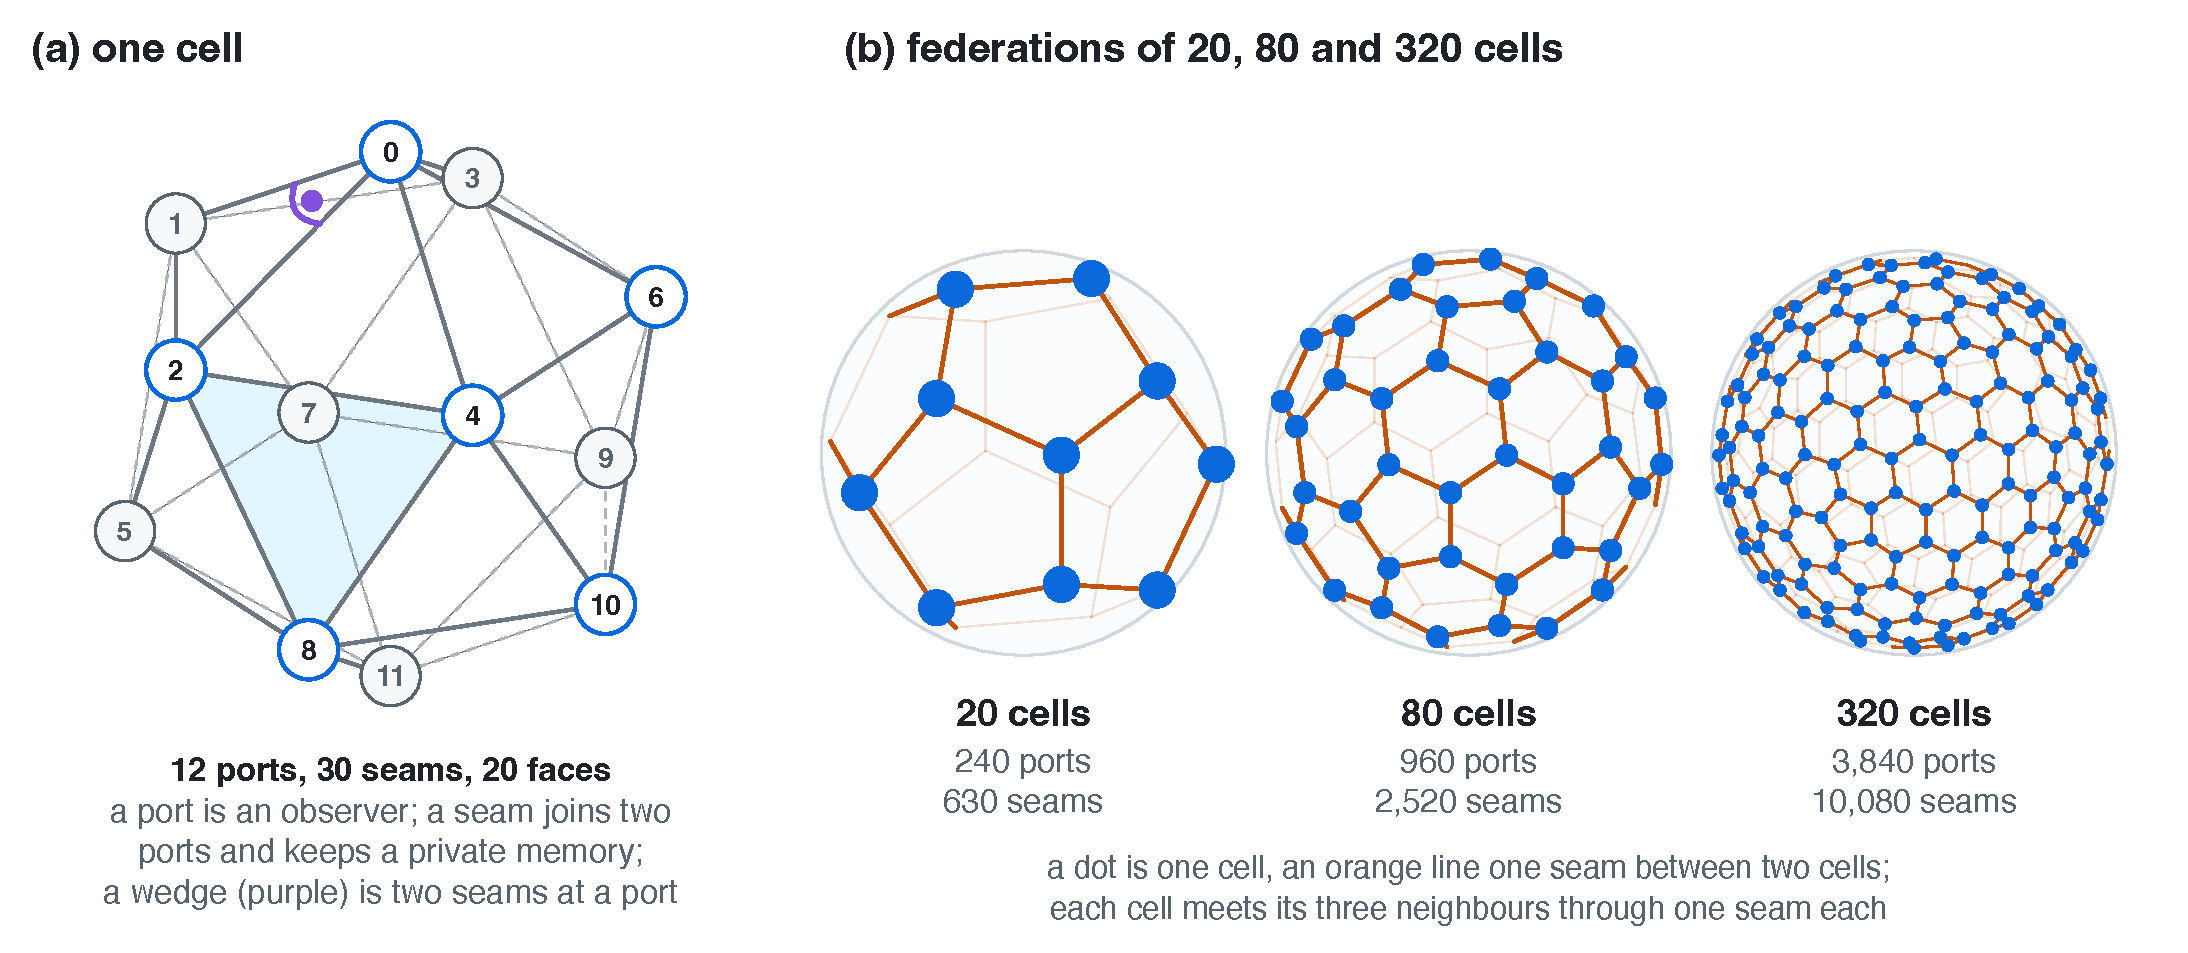
\includegraphics[width=\linewidth]{../paper/figures/model_hardware.pdf}
\caption{The hardware of the computation. (a) One cell: twelve ports with
the incidence of the icosahedron, thirty seams and twenty faces, with one
face shaded and one wedge, two seams at a port, marked. The cell is one
observer and its ports are its interfaces; every seam joins two ports and
keeps a private memory. (b)
The federations of $20$, $80$ and $320$ cells; one dot is one cell, and one
line is the external seam between two neighboring cells. Ports, seams and
cells are registers of a computation and no space.}
\label{fig:model-hardware}
\end{figure}

The emitter is local. One fuel state at a seam $e=(a,b)$ has energy
$E_f=10\kappa+(d_a+d_b-2)/2$ and couples with strength $g$ to the pair on
that seam. A pulse of duration $\pi/(2g)$, with the law acting throughout,
converts the fuel into the pair with an error of at most
$\sqrt{d_a+d_b-2}/(2g)$ in norm. No level of the law is prepared.

The reader is the agreement of the two ends of a seam. Each end copies the
predicate ``both ends hold one
load'' into a private pointer, a courier carries one copy, and a record is
admitted only when both copies are valid and agree. A public comparison
copies an orthogonal classical outcome of a complete
instrument. It does not copy an arbitrary private quantum state. On $20$
cells the complete set of outcomes is one record for each of the $630$
seams and one outcome ``no pair''; fuel left in the emitter counts as ``no
pair''. The complete readout executed with the two-load sector of one cell
and the fuel has a total-variation error of $2.09\times10^{-7}$. The seam
memory stays private and unread. Each reading uses a fresh run, so reading
is never used to hold an object in place.

\subsection{The binding theorem}
\label{sec:binding}

Let $P$ be the span of all pairs on a seam and $Q$ its complement in the
sector of two loads, doubled loads included.

\begin{theorem}[Binding of a pair]
\label{thm:binding}
On every federation of complete cells with a matching of external seams, for $\kappa\geq0$,
\begin{equation}
 PH_\kappa P\le(10\kappa+6)\,P,\qquad
 QH_\kappa Q\ge12\kappa\,Q,\qquad
 \|QH_\kappa P\|\le\sqrt{10}.
\label{eq:binding-blocks}
\end{equation}
For $\kappa>3$, every state that starts in $P$ obeys, at every value $t$
of the evolution parameter,
\begin{equation}
 \Pr(\text{no pair on a seam};t)\le\frac{40}{(2\kappa-6)^2}.
\label{eq:binding-bound}
\end{equation}
The bound is independent of the number of cells.
\end{theorem}

\begin{proof}[Idea of the proof]
The costs $10$, $12$ and $24$ set the diagonal parts of the two blocks.
Inside $P$ the exchange takes a pair on one seam to pairs on the seams
that share a face with it. This motion graph is the line graph of the
dodecahedral dual of the cell, whose adjacency is at least $-2$, and the
exchange diagonal is at most $5$, which gives the bound $6$. A pair on an
external seam has no such partner. In the coupling, a state of $P$ reaches
states of $Q$ with total weight at most $5$ and a state of $Q$ reaches
states of $P$ with total weight at most $2$, which gives $\sqrt{10}$. Put
$a=10\kappa+6$, $c=12\kappa$, $\gamma=c-a$ and $\beta=\|QH_\kappa P\|$. The
min-max principle with the two blocks as trial spaces places the lowest
$\operatorname{rank}P$ levels at or below $a$ and all others at or above
$c$. For the projector $\Pi$ on these levels, $Q\Pi$ solves a Sylvester
equation with ordered spectra, so $\|Q\Pi\|\le\beta/\gamma$, and
$\|(I-\Pi)P\|\le\beta/\gamma$ in the same way. A state that starts in $P$
therefore has amplitude at most $2\beta/\gamma$ outside $P$ at every $t$,
and probability at most $4\beta^2/\gamma^2$. No spectral projector is an
operation of an observer; $\Pi$ belongs to the proof.
\end{proof}

The bound applies to the first read after any chosen interval of
uninterrupted evolution. A conditioned sequence of measurements requires
the intervening instruments in the calculation. On the federations of $20$, $80$
and $320$ cells the largest level of the adjacent block of the exchange is
$5.7008$, $5.7000$ and $5.7000$ against the bound $6$, and the largest
singular value of the coupling is $2.0821$, $2.0811$ and $2.0822$ against
$\sqrt{10}\approx3.1623$. Exact integer bounds on these three
carriers give $17.35/(2\kappa-5.701)^2$ for $2\kappa>5.701$. On
one cell the two constants are $5$ and $2$. With the emitter at
$\kappa=128$ and $g=64$, the outcome ``no pair'', which includes a doubled
load and fuel left in the emitter, has probability at most
$64009/25600000\approx0.0025$ at the first read after any free interval, for an emitter on any
seam of such a federation.

\subsection{Particle stability}
\label{sec:particle-stability}

The model reproduces particle stability as an observable: a bound object
persists in free evolution, read on the agreed records of the port
observers. The claim on records has four parts. A pair of loads written on
one seam by the local emitter is read as a pair on some seam with
probability at least one minus the bound after any chosen free interval up to the first read. It is read on
other seams than the first. Nothing holds it but the law. The same law
with the agreement energy removed loses it.

\begin{table}[htbp]
\centering\small
\caption{Particle stability in the agreed seam records, emitter coupling
$g=64$. The bound is that of Theorem~\ref{thm:binding} with the constants
of the carrier and the error of the emitter. Each probability is the
largest value across the sampled waits. Each wait uses a fresh preparation. The federation of $320$ cells is run at
$\kappa=8$.}
\label{tab:particle-stability}
\begin{tabular}{@{}lcccccc@{}}
\toprule
 & \multicolumn{3}{c}{$\kappa=8$} & \multicolumn{3}{c}{$\kappa=128$}\\
\cmidrule(lr){2-4}\cmidrule(l){5-7}
\textbf{Carrier} & bound & no pair & another seam & bound & no pair & another seam\\
\midrule
one cell & $0.148790$ & $0.00956834$ & $0.985996$ & $0.001447$ & $0.00001881$ & $0.991270$\\
$20$ cells & $0.182975$ & $0.00962164$ & $0.977029$ & $0.001606$ & $0.00002270$ & $0.933194$\\
$80$ cells & $0.182787$ & $0.00964389$ & $0.977130$ & $0.001605$ & $0.00002270$ & $0.933194$\\
$320$ cells & $0.182965$ & $0.00963435$ & $0.977091$ & & & \\
\bottomrule
\end{tabular}
\end{table}

Table~\ref{tab:particle-stability} gives the readings, and
Figure~\ref{fig:model-stability} follows them through the run on $20$
cells. The probability of
``no pair'' lies a factor of ten and more below the bound on every
carrier, and the largest probability of reading the pair on another seam
than the emitter's lies between $0.93$ and $0.99$.

\begin{figure}[!htb]
\centering
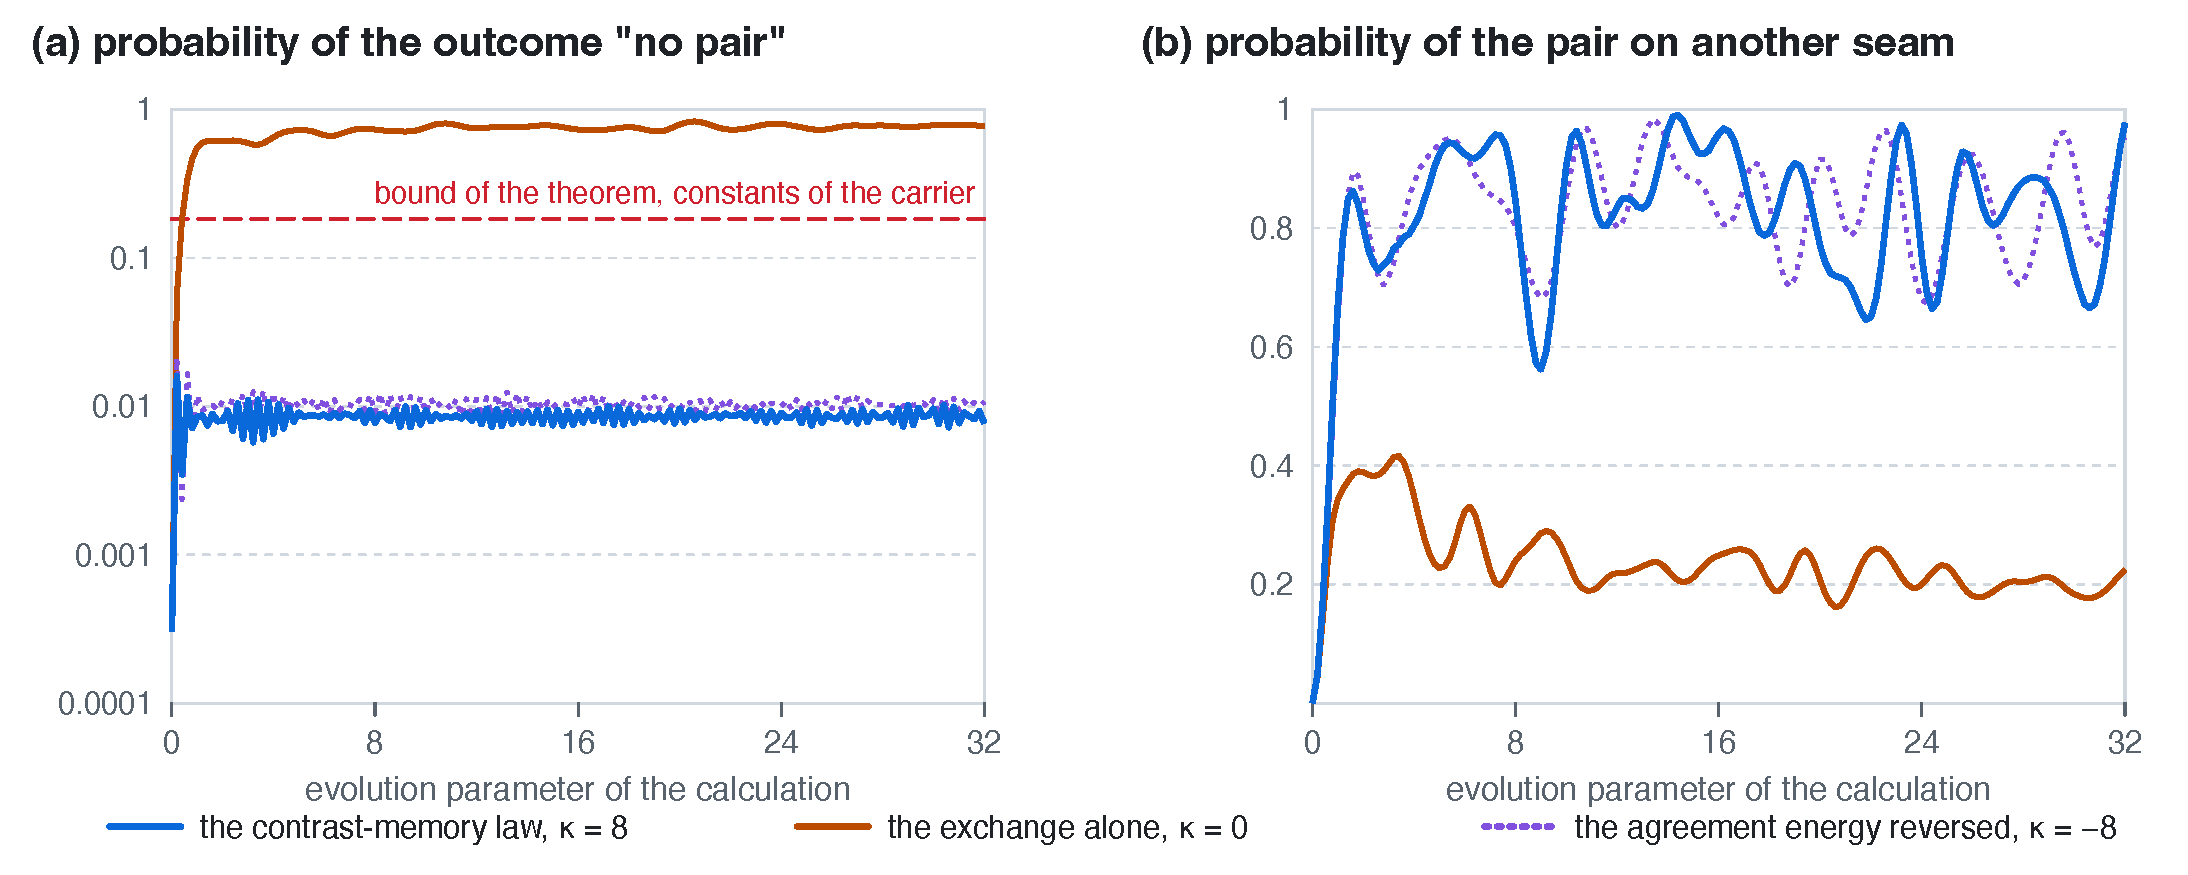
\includegraphics[width=\linewidth]{../paper/figures/model_stability.pdf}
\caption{Particle stability on the federation of $20$ cells, with the pair
written by the local emitter on one seam at $\kappa=8$ and its two
changed laws. (a) The probability of the outcome ``no pair'' on a
logarithmic scale, with the bound of Theorem~\ref{thm:binding} for the
constants of the carrier. (b) The probability of reading the pair on
another seam than the emitter's. Each point is the probability of a record
at one reading; the $161$ values of the evolution parameter are those of
the calculation. The largest values of ``no pair'' on this grid are
$0.0160$ under the law, $0.830$ under the exchange alone and $0.0211$ with
the agreement energy reversed; at the readings $0,4,\dots,32$ used in the
text they are $0.0096$, $0.7968$ and $0.0124$.}
\label{fig:model-stability}
\end{figure}

A second experiment prepares two adjacent unit loads directly and releases
them on the full $20$-cell sphere with blank memories. After $37$ exchange
time units a single cell reads an adjacent pair on one of its thirty
internal seams with probability $0.98027$ at $\kappa=8$, $0.20291$ at
$\kappa=0$ and $0.98389$ at $\kappa=-8$. An independent assembly of the
$28{,}680$-state generator and Chebyshev propagation reproduce the local
outcome probabilities at the positive coupling and at zero.\footnote{The
\href{https://github.com/openwave-labs/openwave/blob/753232cac4976ab2ca208eb99d73fe7ac88ef333/openwave/xperiments/m10_oph/research/findings/m10_3_maintainer_review.md}{independent numerical review}
specifies the board, release, propagator and complete receiver distribution.}
The theorem places the adjacent band below two free unit loads at
$\kappa=8$, and the same patch can resolve the sign of the interaction,
which an adjacency reading by itself accepts either way. Two half
contacts split the pair coherently across three configurations, and a
third recombines two alternatives before the patch reads the launch
seam. At exposure $1/16$ the click probabilities are $0.44007$ and
$0.02407$ at $\kappa=+8$ and $-8$, and the corresponding incoherent
mixture reduces their difference from $0.4160$ to $0.00051$
\cite{ophmodel}.

\subsection{Events with each observer's own count}
\label{sec:events}

The runs above use the sum of the seam terms with a continuous parameter.
As local events the law needs no common clock. One event is one seam
acting once,
\begin{equation}
 \exp\Bigl(-i\tau\Bigl[\frac{I-\mathrm{SWAP}_e}{2}-2\kappa\,n_an_b\Bigr]\Bigr),
\label{eq:seam-event-unitary}
\end{equation}
with event angle $\tau$. Each port counts the events of its own seams, and
these counts are the local clocks of its cell.

The records depend on the local order of events alone. Two sequences in
which every port sees its events in the same order give the same seam
records exactly, and no order between events that share no port enters a
record. At $\kappa=8$ and event angle $1/64$, rounds in which every seam
acts once in a fresh random order keep the pair, with largest ``no pair''
probability $0.0217$ on one cell and $0.0188$ on $20$ cells, and so do
rounds in which half of the carrier acts twice, $0.0470$ and $0.0268$.
The counts of
different ports differ by up to a factor $2.6$, and no common count
exists. Seams that act independently at random lose the pair at these
angles, $0.5048$ on one cell and $0.1989$ on $20$ cells, and the loss
falls with the angle, to $0.1897$ on one cell at $1/256$.

Committing the label also loses the pair. With the contrast of the acting
seam committed to a public record at every event, the probability of ``no
pair'' on one cell grows to $0.32$ after $2048$ rounds; unread, its
largest value is $0.018$. The binding rests on the regular phase between
successive events of a seam, and an observer that serves each of its
seams once per round supplies that regularity with its own count.

Overlapping observers agree on what they share. On the $320$-cell
sphere, $320$ single-cell observers and $960$ overlapping three-cell
observers of Interval Echo track $34$ conserved mobile doubles through
$2{,}399$ transfers, and every reading of a shared checkpoint agrees. Two
repairs that compete for one doubled port leave distinguishable records,
and a prepared local priority makes both request orders end in one common
terminal state. On the $20$-cell sphere two overlapping two-cell observers
realize the unique weighted information projection of the supplied
preparation to a uniform reference in both orders \cite{ophmodel}.

\subsection{What a reading leaves}
\label{sec:presence}

Two instruments agree on the first answer to the question of whether
a pair occupies some seam. For the thirty seam projectors $P_e$, put
$P=\sum_e P_e$. One instrument combines the seam readings, copies a single
answer and reverses its scratch work. The other keeps the individual
seam records (Figure~\ref{fig:model-run}). Their respective positive
operations are
\begin{equation}
X\longmapsto PXP
\qquad\text{and}\qquad
X\longmapsto\sum_eP_eXP_e .
\label{eq:presence}
\end{equation}
Both give the same first probability. Four further units of exchange
make their difference visible. A positive first answer followed by a
return to the emitting seam has probabilities $0.0182640$ and $0.1029264$.
Including finite read windows, the two public histories differ by more
than $0.0817$ in total variation \cite{ophspine}.

\begin{figure}[!htb]
\centering
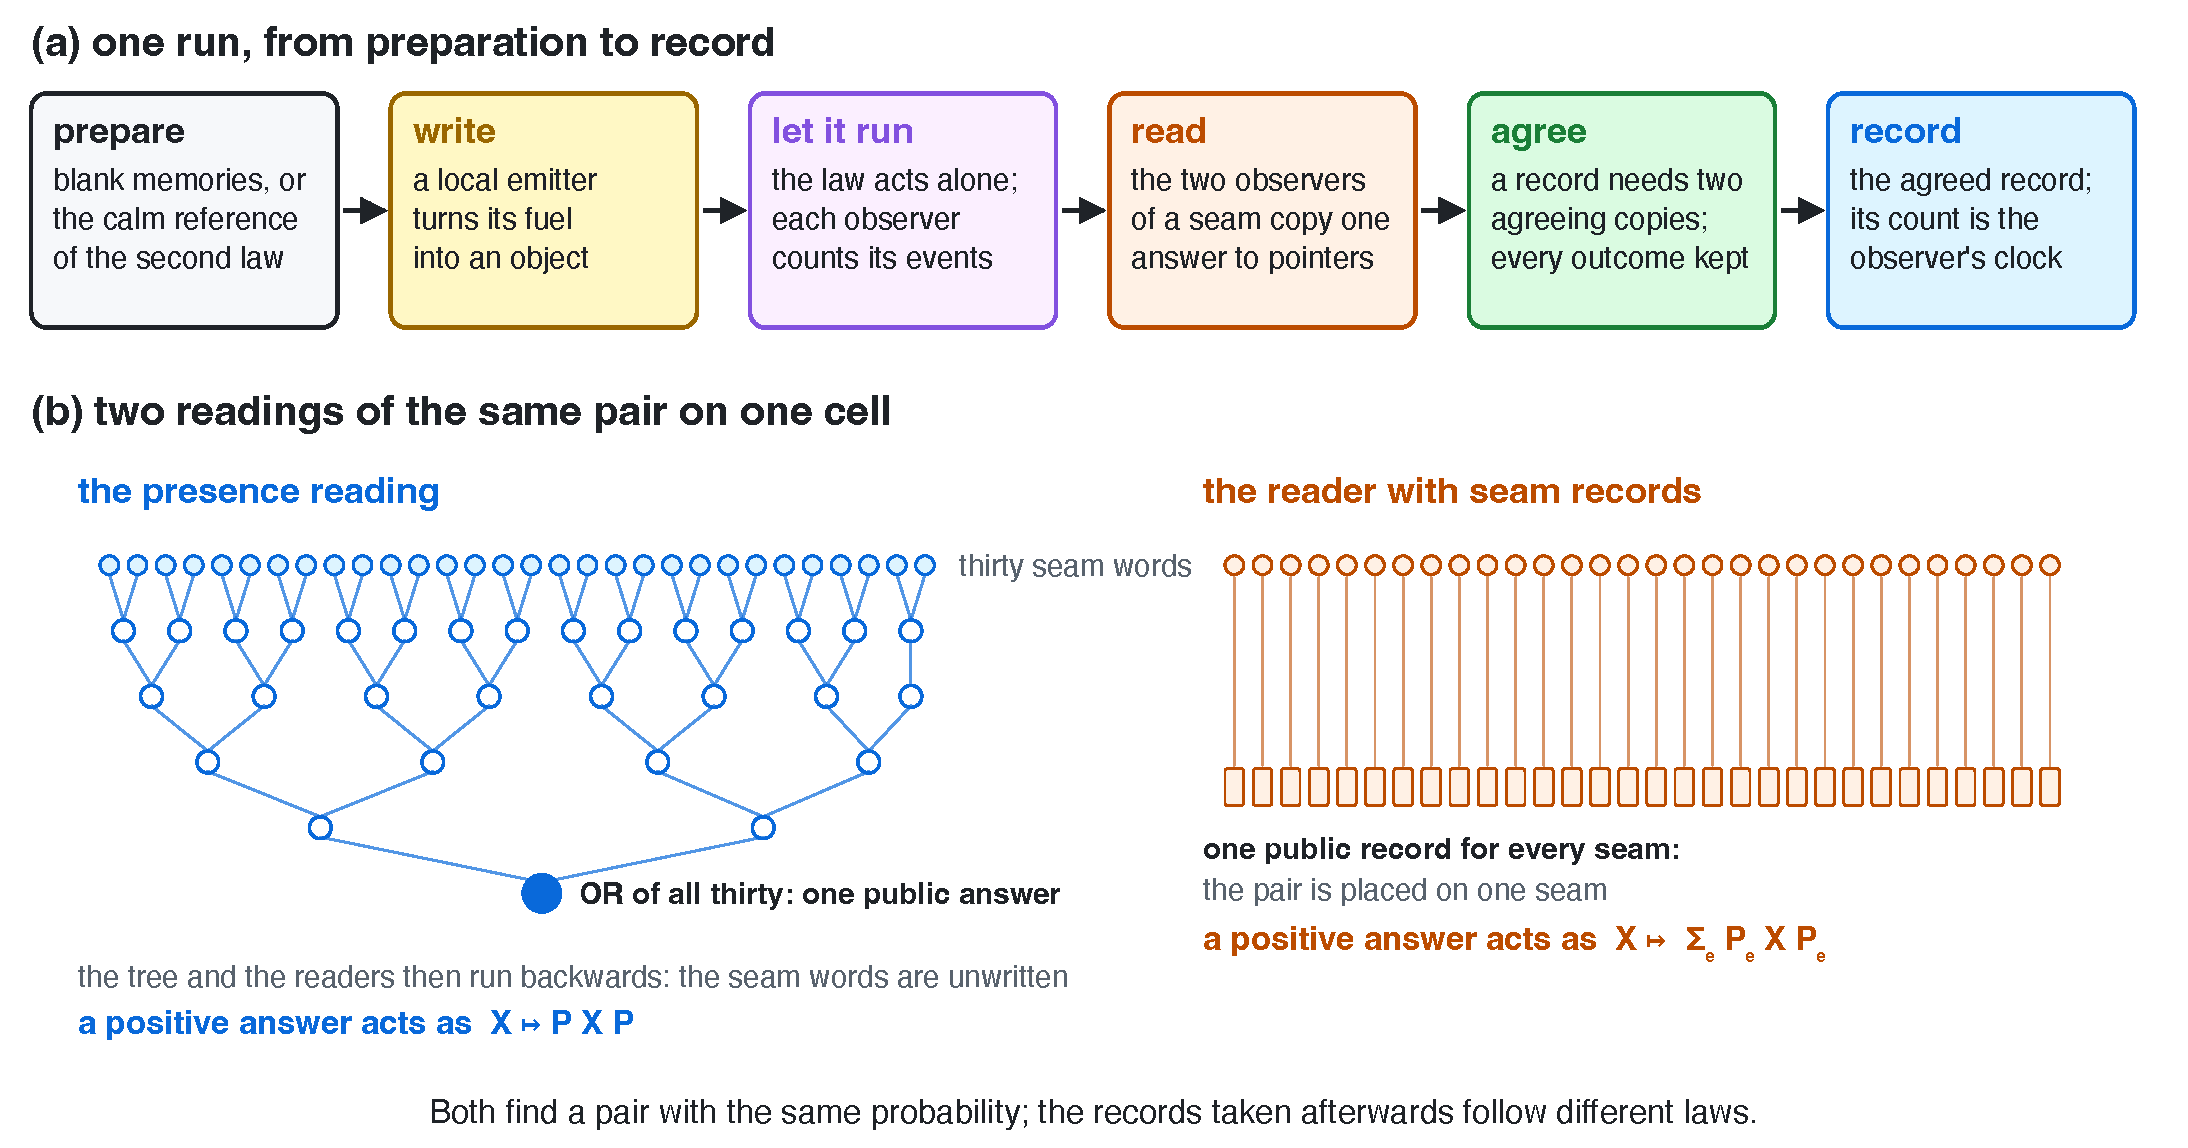
\includegraphics[width=\linewidth]{../paper/figures/model_run.pdf}
\caption{Observers, instruments and records. (a) One run of the model, the
same for every candidate law: a preparation, a local write by an emitter, the law
acting alone while every observer counts its own events, a reading copied
into two pointers, agreement of the two copies, and the agreed record whose
count is the observer's clock. (b) Two readings of the same pair on one
cell. The presence reading combines the thirty seam words by a reversible
tree, copies one answer and unwrites the words; the reader with seam
records keeps thirty records. The next reading distinguishes the two histories.}
\label{fig:model-run}
\end{figure}

On Interval Echo, observers test the same distinction for six pairs of
addresses with four stations that each read a bit twice. The simulated
records bound the difference of any later public event on the enrolled
code from the ideal pair reading by $0.0910$ at joint $99\%$ confidence,
while a reader that also records the address and forgets it publishes the
same pair name and errs by more than $0.4813$ on a tested event
\cite{ophspine}.

\subsection{Bound objects of the contrast-memory law}
\label{sec:bound-objects}

Under the law \eqref{eq:contrast-law} an object is a set of loads. A load
counts $6$ in $C$ and every agreed seam takes $2$ off, so an object of $N$
loads with $m$ agreed seams costs $6N-2m$.
Table~\ref{tab:bound-objects} lists the cheapest objects on one cell. The
first three are a port, a seam and a face, the three kinds of centre of
the cell: $12$ ports, $30$ seams and $20$ faces, $62$ axis points in all.
Every object gains at least $2$ against every split into two parts.

\begin{table}[htbp]
\centering\small
\caption{The cheapest objects of $N$ loads on one cell under the
contrast-memory law. The cost is the value of $C$; the last column is the
least gain in $C$ against a split into two objects.}
\label{tab:bound-objects}
\begin{tabular}{@{}rlrrrr@{}}
\toprule
$N$ & \textbf{Shape} & \textbf{Number} & \textbf{Agreed seams} & \textbf{Cost} & \textbf{Gain}\\
\midrule
$1$ & one port & $12$ & $0$ & $6$ & \\
$2$ & one seam & $30$ & $1$ & $10$ & $2$\\
$3$ & one face & $20$ & $3$ & $12$ & $4$\\
$4$ & two faces on a seam & $30$ & $5$ & $14$ & $4$\\
$5$ & three faces round a port & $60$ & $7$ & $16$ & $4$\\
$6$ & a port and its five neighbours & $12$ & $10$ & $16$ & $6$\\
$12$ & the whole cell & $1$ & $30$ & $12$ & $10$\\
\bottomrule
\end{tabular}
\end{table}

At finite coupling the lowest level of $N$ loads on one cell lies below
$N$ free loads. At $\kappa=8$ the binding is $14.236$, $43.728$,
$75.212$, $107.678$ and $155.076$ exchange units for $N=2$ to $6$, and in
the lowest level of two loads the pair is on a seam with probability
$0.99$; these levels are audit on the spectrum. Inside a cell the exchange
takes a pair from one seam to the seams of the adjoining faces at first
order, and from the seams of one cell to those of the next the transfer
passes through one separated state with amplitude $1/(8\kappa)$. These
objects are read on ports, seams and faces by the observers of their
cells, and what they need for a physical reading is listed in
Section~\ref{sec:scoreboard}.

\subsection{Matter waves with a rest frequency}
\label{sec:matter-waves}

Loaded port pairs can also carry a wave. Interval Echo has one in
commissioned matter. On a strand of loaded port pairs, each holding one
unit of load, a reversal of the alternating orientation of the
pairs travels from cell to cell while the connecting seam memories stay
coherent and unread. Observers measure its wave number from receiver
profiles and its angular frequency against a local clock made of one
pair. Separate exchange and conditional-phase instruments predict a rest
frequency of $15.00051$ and a squared speed of $16.00156$ in these
units. On three reserved boards of $20$, $80$ and $320$ cells, the two
coupling measurements forecast $22$ frequencies within $0.000575$ of the
lattice relation, and the $14$ lines with wave number at most $0.50$
agree within $0.003165$ with the Klein--Gordon relation
$\omega^2=\omega_0^2+c^2k^2$, against a tolerance of $0.0048$ that a
tangent parabola also meets on that range. Each measured spatial profile passes its
held test, while the wavelengths used to launch the waves fail the same
test on every board \cite{ophspine,ophmodel}. The strand is
one-dimensional collective matter. Its long-wave coefficient corresponds
to a speed of four strand steps per clock unit while the fastest
measured packet travels at $0.99$, so the band has the Klein--Gordon
form at long wavelengths without fixing one limiting speed.

\subsection{The scalar channel: an object with a clock}
\label{sec:cage}

In a separate candidate on the same carrier, a local observer can measure
both an object's oscillation and the energy difference responsible for it.
One mode lives on each seam and one on each pair of seams that meet at a
port. Let $C$ be their signed incidence matrix. The one-object generator
and its parameters are
\begin{equation}
 D=\begin{pmatrix}m&cC\\ cC^{\top}&-m\end{pmatrix},
 \qquad m=1,\quad c=1/\sqrt{2}.
 \label{eq:scalar}
\end{equation}
On four seams forming a ring of degree-five ports, take the alternating
profile $e=(u_{ab}-u_{bc}+u_{cd}-u_{da})/2$. Its signed contributions
cancel at each port. Hence $CC^{\top}e=10e$, and the span of $e$ and
$C^{\top}e/\sqrt{10}$ has energies $\pm E$, with
$E=\sqrt{m^2+10c^2}=\sqrt{6}$. Promotion from the occupied lower mode
to the upper mode costs $2E$. Its occupation is conserved, while a
superposition can produce an oscillating local reading. The specialist
paper gives the proof for number-conserving measurements, the register
construction and the pulse protocols \cite{ophspine}.

The observer uses a local circulating mode as a phase reference. After
the preparation pulse, counts on the ring yield a free oscillation of
$4.898982\pm0.000002$ in that reference's units. A separate adjustable
fuel level resolves the gap at $4.898980\pm0.000008$. Both measurements
agree with $2\sqrt{6}$. Adding hopping around each port preserves
the cell symmetries and particle number, but the best single frequency
then accounts for only $50.7\%$ of the variance. This comparison
identifies a localized two-level clock in the scalar channel.

%=====================================================================
\section{Forces and the particle classes}
\label{sec:gauge}

A desktop with particles also needs forces between them and labels that
tell the particles apart. On the twelve-port cell, the forces come from
the currents that observers can drive at the ports, and the labels from
the defects that repair leaves behind. A finite theorem fixes
the Lie type of a complete current algebra under explicit response
premises, and the chosen memory law then realizes its currents. These
are different steps of one construction: the Lie type constrains
admissible interactions, while the executable specification fixes what
its port services generate. The protected defects carry exactly the
centre classes of the Standard Model particles.

\subsection{The finite gauge theorem and matter representation}

Let $A$ be the icosahedral adjacency matrix and $J$ its antipodal involution.
Exact incidence gives
\begin{equation}
10J=A^3-4A^2-5A+10I,
\qquad P_{12}=\mathbf1\oplus\mathbf5\oplus\mathbf3\oplus\mathbf3'.
\label{eq:antipode-polynomial}
\end{equation}
The even port coordinates carry $\mathbf1\oplus\mathbf5$; the odd coordinates
carry the two triplets. The response premise of Section~\ref{sec:no-outside}
requires an injective derivative $D:P_{12}\to\mathfrak u(H)$, a
commutator-closed image with positive trace pairing, and internal implementation
of every proper carrier rotation. Internal implementation means that its
projective implementer factors into the connected response group and a
pointwise centralizer. This is the response-endogeneity clause identified
as A2 in the library; it is not implied by the port count alone
\cite{ophbasis,ophGauge}.

\begin{theorem}[Gauge Lie-type forcing]
\label{thm:inner-action-closure}
\leavevmode\par
Under these complete-response and internal-implementation premises,
\[
 \mathfrak g=D(P_{12})\cong
 \mathfrak u(1)\oplus\mathfrak{su}(2)\oplus\mathfrak{su}(3).
\]
Its center is the uniform port line. The three-dimensional simple ideal
carries one triplet, and the eight-dimensional ideal carries the other
triplet and the five-dimensional band.
\end{theorem}
\begin{proof}
The trace pairing makes the twelve-dimensional image compact. Internal
implementation makes the $A_5$ action inner, so it fixes the center
pointwise. The transitive port action has a one-dimensional fixed space,
hence the center has dimension at most one. With zero center, the only
compact semisimple type of dimension twelve is $\mathfrak{su}(2)^4$.
Inner automorphisms preserve its simple ideals, each of which has either
zero or three $A_5$-fixed directions, contradicting the one-dimensional
fixed space. The center therefore has dimension one; the unique compact
semisimple type of dimension eleven is
$\mathfrak{su}(2)\oplus\mathfrak{su}(3)$ \cite{hall2015}.
\end{proof}

The premises have an explicit finite matrix realization. Six antipodal
axis vectors form a matrix $U$ over $\mathbb Q(\sqrt5)$; $\sigma(U)$ is its
Galois conjugate. For even coordinates $b$, odd coordinates $d$, and
$c=\frac16\sum_i b_i$, put
$\Phi_0(b-c\mathbf1)=\sum_i(b_i-c)u_iu_i^{\mathsf T}$.
For nonzero real band coefficients,
\begin{equation}
 K(f)=\operatorname{diag}\!\left(
 \lambda_3\widehat{Ud}
 +i[\lambda_1cI_3+\lambda_5\Phi_0(b-c\mathbf1)],
 \lambda_{3'}\widehat{\sigma(U)d}\right),
 \qquad \widehat{x}y=x\times y .
\label{eq:port-response-map}
\end{equation}
\begin{proposition}[Finite response realization]
\label{thm:finite-response}
The map $K$ is injective and equivariant, its image is commutator-closed,
and proper carrier rotations act internally. Its pulled-back bracket has
\begin{equation}
 (P_{12},[\ ,\ ]_K)\cong\mathfrak u(3)\oplus\mathfrak{so}(3).
\label{eq:liealgebra}
\end{equation}
\end{proposition}
The six axis projectors span the symmetric matrices, while the triplets
span the skew matrices in the two blocks. These rank and equivariance
identities are exact over the full sixty-element rotation group. The
representation and nonzero coefficients are design inputs. A zero bracket
on the same port module violates the internal-implementation premise;
it is not excluded by geometry alone. The gauge specialist gives the
complete finite certificate and the boundary between analytic classification
and machine-checked algebra \cite{ophGauge}.

\begin{theorem}[Finite matter image]
\label{thm:matter-image}
For the supplied trace-balanced module
$V=\mathbb C^3_{-1/3}\oplus\mathbb C^2_{1/2}$,
\begin{equation}
 \Lambda^2V\oplus\Lambda^4V
 =Q\oplus u^c\oplus e^c\oplus d^c\oplus L,
\label{eq:generation}
\end{equation}
where $Q=(3,2)_{1/6}$, $u^c=(\bar3,1)_{-2/3}$,
$e^c=(1,1)_1$, $d^c=(\bar3,1)_{1/3}$ and $L=(1,2)_{-1/2}$.
All perturbative gauge and mixed gravitational anomalies vanish, the number
of weak doublets is even, and the faithful image is
\begin{equation}
 \frac{\mathrm{SU}(3)\times\mathrm{SU}(2)\times\mathrm U(1)}{\mathbb Z_6}.
\label{eq:globalform}
\end{equation}
Among the $1{,}024$ subsets of the ten nontrivial irreducible exterior
summands, nonemptiness, chirality and the four anomaly-trace conditions
select exactly this fifteen-state mask and its charge conjugate.
\end{theorem}
The exterior branching, anomaly traces and center kernel are finite
calculations \cite{ophGauge}. The supplied module is the familiar
$\mathbf{10}\oplus\overline{\mathbf5}$ branching; this result does not
require a physical $\mathrm{SU}(5)$ gauge field. It does not fix the
number of families.

Interval Echo implements the connected group (\ref{eq:globalform}) on a
protected five-level code. Observers program two magnetic bands and their
charge weights, then compare the effects of ordered port phases. An exact
rank certificate shows that the twelve compressed currents span
$\mathfrak{s}(\mathfrak u(3)\oplus\mathfrak u(2))$. The centre is the
circle $\{\operatorname{diag}(e^{2it}I_3,e^{-3it}I_2)\}$, and
$\mathbb Z_6$ is the kernel of the covering product. The order-six subgroup
generated by $e^{2\pi iY}$ supplies the flux alphabet in
Section~\ref{sec:defect-families}. Identifying this action on freely
propagating matter requires measuring which code and charges the material
selects \cite{ophGauge}.

\subsection{The port response of the executable model}
\label{sec:port-response}

Theorem~\ref{thm:inner-action-closure} consumes twelve port generators
that are independent, closed under commutators and carry a positive trace
form, with the rotations of the cell acting through them. The
contrast-memory law on one cell is tested against this premise. A port
service is a weak operation by the observer of one port that lasts long
against the inverse level spacings of the law, so that it acts through its
part diagonal in the levels. The response space is the pair of triplets
$\mathbf 3\oplus\mathbf 3'$ of \eqref{eq:bands}: for one load the slow and
the fast level of Section~\ref{sec:contrast-memory}, for the bound pair
its two lowest triplets that are odd under the antipodal map. The matrices
of this subsection are audit, and no observer reads them.

The plain services of the law are the load of each port, the exchange of
each seam and the twist of each port, its circulation round the five
neighbours. The loads alone generate seventeen dimensions, two copies of
$\mathfrak{su}(3)$ and one common number, and all plain services together
generate eighteen. The count follows from a lock between the two triplets:
every operator at a port with rational entries acts on the fast triplet as
the conjugate under $\sqrt5\mapsto-\sqrt5$ of its action on the slow
triplet.

One declared service gives twelve. Let $H_1=L/2$ be the law of one load
without its constant, $E_{\rm top}=(5+\sqrt5)/2$ its top level and $J_v$
the twist of port $v$, and put
\begin{equation}
 F_v=\tfrac12\bigl\{n_v,\,E_{\rm top}-H_1\bigr\}+J_v .
\label{eq:declared-service}
\end{equation}
The twelve $F_v$ are independent and close under commutators into
$\mathfrak u(3)$ on the slow triplet and $\mathfrak{so}(3)$ on the fast
one, the form \eqref{eq:liealgebra}. Their trace form is positive, the
$66$ brackets lie inside the span with residual $9\times10^{-15}$, and the
$720$ covariance identities of the $60$ rotations hold with residual
$2\times10^{-15}$. The weighting, whose coefficient is tied to a level of
the law, and the twist are supplied.

Interval Echo selects its port service from the rotations of the cell. The
twelve rotations by a fifth of a turn sum to a class operator, and its
positive spectral projector $P$ selects the response; the service of port
$p$ is the band-diagonal part of $Pn_pP+J_p$ with unit gain. On one load
and on the bound pair at $\kappa=8$ the twelve services are independent,
all $66$ brackets lie in their span, and the $720$ rotation-conjugation
checks hold with residual norms below $10^{-11}$. Prepared overlap
transport generates all $60$ proper rechartings on $20$ and $80$ cells with
a matching unit-gain implementer. A signed pulse of the current at one port
changes the distribution of the bound pair's seam readings by up to $0.11$
in total variation, so the observers of the cell read these currents.
Admitting the bare load of a port as a further service enlarges the visible
closure to $17$ directions, and the completeness of the physically
accessible menu is the premise on which the inference to the gauge algebra
rests \cite{ophmodel}.

\subsection{Protected centre classes}
\label{sec:defect-families}

A protected defect on a carrier face holds a flux class
$k\in\mathbb Z_6=\mathbb Z_3\times\mathbb Z_2$,
a colour-centre charge with a weak-centre parity, and the classes on one closed carrier add to zero. A
quantum's internal pattern is an occupation $(n_3,n_2)$ of the five-level code
$V=\mathbb C^3_{-1/3}\oplus\mathbb C^2_{1/2}$, with $6Y=3n_2-2n_3$.

\begin{theorem}[Native flux and centre-character dictionary]
\label{thm:defect-classes}
The kernel element $(\omega I_3,-I_2,e^{2\pi iY})$ of the covering product acts as the
identity on all $32$ patterns, and a flux of class $f$ acts on a pattern by the phase
$e^{2\pi if\cdot6Y/6}$. The class seen by a pattern is
\[
 k\equiv 6Y \pmod 6,\qquad k\bmod 3=n_3\bmod 3,\qquad k\bmod 2=n_2\bmod 2,
\]
and the class multiplicities are $(4,6,6,4,6,6)$.
\end{theorem}
\begin{proof}
$\omega I_3$, $-I_2$ and $e^{2\pi iY}$ act by $\omega^{n_3}$, $(-1)^{n_2}$ and
$(-1)^{n_2}\omega^{-n_3}$; the rest is reduction of $6Y$ modulo $3$ and $2$.
\end{proof}

\begin{table}[htbp]
\centering\small
\caption{Native flux classes and compatible Standard Model centre characters. A class does not uniquely identify a physical species.}
\label{tab:defect-families}
\begin{tabular}{@{}cll@{}}
\toprule
$k$ & Centre characters & Particles\\
\midrule
$1,5$ & $\omega^{\pm1},\,-1$ & left-handed quarks $Q$ and antiquarks\\
$4,2$ & $\omega^{\pm1},\,+1$ & right-handed quarks and antiquarks\\
$3$ & $1,\,-1$ & lepton doublet and Higgs doublet\\
$0$ & $1,\,+1$ & $e_R$, $\nu_R$, photon, gluons, $W$, $Z$\\
\bottomrule
\end{tabular}
\end{table}

A quantum of class $k$ taken around a flux of class $f$ gains the phase $e^{2\pi ifk/6}$,
so colour flux is seen only by quarks and weak flux only by the weak doublets, the
left-handed fermions and the Higgs. The
central involution $z$ of the carrier's rotation cover acts on the code as
$\operatorname{diag}(1,1,1,-1,-1)=e^{i\pi\cdot6Y}$.

The class is the centre class. It carries neither the generation nor $T_3$, so up and down,
electron and neutrino, and colour singlet and octet share a class. The executable certificates check every
pattern in exact arithmetic \cite{ophparticles,ophrepo}.

The same code fixes the couplings of the links at the cell. The seam cost of
a code state carried around a plaquette, averaged over the code, is
$1-\operatorname{Re}\operatorname{tr}_5U_P/5$, and this trace gives equal bare
couplings $g_3=g_2=g_1$ in the grand-unified normalization at the cell, so
$\sin^2\theta_W=3/8$ there, and gluons, $W$ and $B$ travel on one cone.
Restricted to a colour holonomy $W$ the cost is
$(3/5)(1-\operatorname{Re}\operatorname{tr}W/3)$, the Wilson plaquette action
with $\beta=6/g^2$, and the colour centre is the pair of flux classes $2$ and
$4$. A Monte Carlo study of these links at $N_t=4$ finds a first-order
deconfinement transition at $\beta_c=5.69105(39)$, where the published value
for this lattice theory is $5.6925(2)$ \cite{ophGauge,boyd1996thermodynamics}.
The equality holds for the bare couplings of this action, and the study holds
the links alone at one lattice spacing.

\subsection{The field law of a seam connection}
\label{sec:fields}

For the separate seam-field construction, write $D$ and $C$ for the seam-by-port
gradient and face-by-seam curvature, so that $CD=0$.

\begin{theorem}[Local Maxwell selection]
\label{thm:maxwell-selection}
A real quadratic seam action $S(A)=\mathrm{const}+\ell^{\mathsf T}A+\tfrac12A^{\mathsf T}HA$
that is gauge invariant, has off-diagonal Hessian entries only between seams of one face,
and is covariant under the sixty carrier rotations is exactly
$S=\mathrm{const}+\tfrac\kappa2\|CA\|^2$. For positive weights $\epsilon,\beta$, a real linear
autonomous evolution with $\dot B=-CE$, conserved $(\epsilon\|E\|^2+\beta\|B\|^2)/2$ and
reversal with $E$ even and $B$ odd is exactly $\dot E=(\beta/\epsilon)C^{\mathsf T}B$ on closed
flux.
\end{theorem}

\begin{proof}
Gauge invariance is $HD=0$ and $D^{\mathsf T}\ell=0$. At an edge of a face and its opposite
vertex, locality permits exactly the other two edges in that entry of $HD$, and the signs of
$CD=0$ propagate one weight $w_f$ over the face. Subtracting $\sum_fw_fC_f^{\mathsf T}C_f$ leaves
a diagonal matrix annihilating $D$, hence zero. Transitivity on faces equalizes the weights,
and the sum of the sixty signed seam actions vanishes, which removes $\ell$. For evolution,
conservation makes the electric block skew and fixes the cross block on closed flux, and
reversal removes the skew block \cite{ophMicrophysics}.
\end{proof}

Exact rank computations and countercontrols verify the classification. On a supplied
Euclidean domain, the complete equal-weight seam symbol $\Lambda_a$ obeys
$0\leq r^2-\Lambda_a(k)\leq a^2r^4/20$ at $r=|k|$, and its reversible curl-pair group converges
to the local Maxwell group with $\|U_a(t,k)-U_0(t,k)\|\leq\min\{2,|t|a^2r^3/20\}$. The premises,
field identification, coefficients and clock are inputs, and native repair does not select them
\cite{ophMicrophysics}. The action principle itself has a source form. For a strictly positive
row-stochastic kernel $P$, the Markov path law is the exponential tilt of the uniform path
reference by $S_{\log}(\gamma)=-\sum_i\log P(\gamma_i,\gamma_{i+1})$ at multiplier one, and a pair
$(S',\lambda')$ reproduces it exactly when $\lambda'S'=S_{\log}+c$ for a constant $c$; the
statements are checked in Lean, and the committed source chain instantiates them
\cite{ophobservers}.

\subsection{A charge with a field}
\label{sec:charge}

A written-field extension of Interval Echo provides a candidate for this
part of the electron. One load more or less than the filled reference
changes the signed boundary flux by a whole unit in individual transfer
records. With source material held in its launch cell, a material probe
responds 22 cell steps away on a prepared 320-cell federation. A magnetic
twist changes the load's return probability. These results establish a
mobile signed charge coupled to the written field of a modified seam
law \cite{ophmodel}.

On registered blank seams, a signed vacancy carries a coherent orbital
state through two cell boundaries. In a guarded cell, one quantum of
applied magnetic flux gives the vacancy two equal-energy states.
Observers can rotate this doublet and transfer its relative phase into a
region of zero net charge by a local pulse drawing on a material donor.
Recording the vacancy address during conversion destroys most of the
recovered coherence. Interchanging two aligned doublets gives positive
exchange phase. These experiments connect angular response and charge
conversion on the same preparation. Identifying the electron requires
fermionic exchange and intrinsic spin on the same travelling excitation,
followed by an independent rest-energy measurement \cite{ophparticles}.

%=====================================================================
\section{Gravity: the Einstein equation from entropy balance}
\label{sec:einstein}

What would an observer see when matter enters a small region? At the same
small proper radius, a ball of positive spatial scalar curvature contains less
volume than its flat counterpart. To enclose the original volume the
observer must go farther out, yet its boundary has \emph{less} area.
Entropy stationarity predicts the size of this deficit from the matter
inside. Measurements by observers moving in different directions can then
determine the entire curvature--stress relation \cite{jacobson16,ophEinstein}.

Three numbers enter for each observer: the entropy response of the
matter in its ball, the deficit of the boundary area and the stress of
the same matter weighed with independent probes. The theorem below turns
ten such triples into a bound on every component of the Einstein
equation. A material of clock pairs then supplies all three numbers on
shrinking balls, and two quantum fields show that the geometry responds
to a correlation that neither field's own state shows.

\begin{figure}[!htb]
\centering
% Figure: the three measured inputs of the Einstein theorem on one small ball of fixed proper volume.
\begin{tikzpicture}[
  meas/.style={oph box=#1, text width=4.9cm, align=flush left, inner sep=3pt, font=\scriptsize}]
% the ball: flat reference (dashed) and the ball with matter at the same volume (solid, larger radius, smaller area)
\draw[ophgrey, dash pattern=on 2pt off 1.6pt, line width=0.6pt] (0,0) circle (1.05);
\draw[ophnative, line width=0.8pt] (0,0) circle (1.22);
\foreach \p in {(-0.35,0.25),(0.3,0.4),(0.1,-0.3),(-0.45,-0.35),(0.55,-0.1),(-0.05,0.7),(0.62,0.62),(-0.7,0.1)}
  \fill[ophdeclared] \p circle (0.06);
\node[font=\scriptsize, text=ophgrey, align=center] at (0,-1.62) {flat reference (dashed) and\\the ball with matter, same volume};
% three measurements
\node[meas=ophnative, anchor=west] (area) at (2.1,1.0) {\textbf{Area deficit} $a_u$: rulers and clocks find\\less boundary area at the same volume};
\node[meas=ophchecked, anchor=west] (ent) at (2.1,0) {\textbf{Entropy response} $s_u$: records of\\the matter inside the ball};
\node[meas=ophdeclared, anchor=west] (str) at (2.1,-1.0) {\textbf{Stress} $T_{uu}$: the same matter\\weighed with material probes};
\draw[oph arrow=ophnative] (1.25,0.55)--(area.west);
\draw[oph arrow=ophchecked] (1.25,0)--(ent.west);
\draw[oph arrow=ophdeclared] (1.25,-0.55)--(str.west);
% result
\node[oph box=ophgrey, text width=4.4cm, align=flush left, font=\scriptsize, anchor=west] (res) at (7.95,0) {%
  \textbf{Ten moving observers}\\[2pt]
  balance $s_u+\eta\,a_u=0$ and weigh\\
  $s_u=2\pi C_\ell T_{uu}$ on shrinking balls\\[3pt]
  $\Rightarrow\ G_{ab}+\Lambda g_{ab}=8\pi G_N T_{ab}$};
\draw[oph arrow] (area.east)--(res.west);
\draw[oph arrow] (ent.east)--(res.west);
\draw[oph arrow] (str.east)--(res.west);
\end{tikzpicture}

\caption{Gravity as a balance of three measurements on one small ball of
fixed proper volume. With matter inside, the observer must go farther out
to enclose the same volume and finds less boundary area. Entropy
stationarity balances the area deficit against the entropy of the
matter, which the same observer also weighs with material probes. Ten
observers in relative motion turn these balances into every component of
the Einstein equation (Theorem~\ref{thm:einstein}).}
\label{fig:einstein-ball}
\end{figure}

\subsection{One source and two independent measurements}
\label{sec:einstein-inputs}

Use signature $(-,+,+,+)$ and units $\hbar=c=k_{\rm B}=1$. On each refinement
the observers identify the same event and preparation and calibrate their
clocks and rulers in a common tetrad. They may register relative motion
with exchanged signals and transported clocks. A reconstruction from
shared records also suffices if it reproduces the regional measurements
on each moving rest slice, including their proper units. For each unit
future timelike $u$, locate a ball by
proper geodesic distance on its local rest slice $\exp_p(u^\perp)$ and vary
its radius until its measured volume equals $4\pi\ell^3/3$. Repeat this
comparison at successively smaller $\ell$ in every frame. Let $a_u$ be
the boundary area minus its value in a local isotropic vacuum reference
shared by the ten observers, with
$G^{\rm ref}_{ab}=-\Lambda g^{\rm ref}_{ab}$. Let $s_u$ be the vacuum-subtracted
bulk entropy response on that ball. Independently obtain the stress $T_{ab}$
of the same matter from the action governing its propagation,
$T_{ab}=-2(\sqrt{-g})^{-1}\delta I_{\rm matter}/\delta g^{ab}$, in the same
vacuum convention. In a quantum state use its expectation value. The
observers measure energy, momentum flux and work in those regions with
material probes calibrated independently of the entropy and area. They
freeze the ordinary-matter calibration before changing the collar state.

At $p$ the geodesic slice has vanishing extrinsic curvature, so the Gauss
constraint gives $R^{(3)}=2G_{ab}u^au^b$. The proper-volume expansion at
radius $r$ is $(4\pi r^3/3)[1-R^{(3)}r^2/30+o(r^2)]$ and the area is
$4\pi r^2[1-R^{(3)}r^2/18+o(r^2)]$. At fixed volume the radius becomes
$r=\ell+R^{(3)}\ell^3/90+o(\ell^3)$. Substitution gives the area
coefficient $a_u=-C_\ell(G_{uu}-\Lambda)+o(\ell^4)$, where
\[
 C_\ell=\frac{4\pi\ell^4}{15}
       =\int_0^\ell 4\pi r^2\frac{\ell^2-r^2}{2\ell}\,dr .
\]
The integral also fixes the matter coefficient if the ball's measured
modular generator is the stress integral with weight
$2\pi(\ell^2-r^2)/(2\ell)$. The modular first law
$\delta S_{\rm bulk}=\delta\langle K_{\rm ball}\rangle$ then gives the
leading response $2\pi C_\ell T_{uu}$ for a stress variation smooth on
the ball. This identification of $K_{\rm ball}$ with the action stress
is a physical premise. Entropy stationarity independently requires the
edge and centre contribution to be $\eta a_u$ and the total first
variation at fixed proper volume to vanish. A bound on the number of
boundary records supplies a ceiling on entropy. The area and bulk
measurements determine whether their signed variations cancel.

\subsection{Ten observers determine the Einstein tensor}
\label{sec:einstein-theorem}

\begin{theorem}[Ten timelike measurements determine the Einstein residual]
\label{thm:einstein}
At each event use one positive area coefficient $\eta$, calibrated on
ordinary matter, and one reference $\Lambda$ for every observer. With
$G_{uu}=G_{ab}u^a u^b$ and similarly for $T$, suppose the same observations
satisfy three bounds on the ten directions below.
\begin{align}
 |s_u-2\pi C_\ell T_{uu}|&\le e_{\rm b}, &
 |a_u+C_\ell(G_{uu}-\Lambda)|&\le e_{\rm a}, &
 |s_u+\eta a_u|&\le e_{\rm s}. \label{eq:timelike-inputs}
\end{align}
Then in the registered tetrad the symmetric tensor
$X=G+\Lambda g-(2\pi/\eta)T$ obeys
\[
 \max_{\mu,\nu}|X_{\mu\nu}|
 \le \frac{17}{8\eta C_\ell}
       \bigl(e_{\rm b}+\eta e_{\rm a}+e_{\rm s}\bigr).
\]
\end{theorem}
\begin{proof}
Subtract the signed stationarity residual $s_u+\eta a_u$ from the sum
of the signed bulk residual and $\eta$ times the signed area residual.
The result is exactly $\eta C_\ell X_{uu}$. The ten observers have velocities
\[
 e_0,\qquad (5e_0\pm4e_i)/3\quad (1\le i\le3),\qquad
 3e_0+2e_i+2e_j\quad (1\le i<j\le3).
\]
Each has squared norm $-1$. The rest reading gives $X_{00}$, sums and
differences of the two axial boosts give $X_{ii},X_{0i}$, and the three
mixed boosts then give $X_{ij}$. The largest absolute row sum of this
rational inverse is $17/8$, attained on a spatial diagonal. The triangle
inequality gives the stated bound. Other measured velocities work whenever
their ten projections have a controlled inverse \cite{ophrepo,ophEinstein}.
\end{proof}

Take a common sequence $\ell\to0$ with each error $o(\ell^4)$ uniformly on
the ten observers. Assume the stress, tetrads and vacuum reference converge
on matching regions, the metric converges locally in $C^2$ to a nondegenerate
metric $g$, and $\eta$ tends to one positive spacetime-independent
$\eta_*$. The bound vanishes, and the limiting coupling is
$2\pi/\eta_*=8\pi G_N$ with $G_N=1/(4\eta_*)$. Thus
\begin{equation}
 G_{ab}[g]+\Lambda g_{ab}=8\pi G_NT_{ab}. \label{eq:einstein}
\end{equation}
For a $C^3$ metric and $C^1$ stress the contracted Bianchi identity,
metric compatibility and the matter action's independent Ward identity
$\nabla^a T_{ab}=0$ give $\partial_b\Lambda=0$. A vacuum measurement at one
event fixes its value on a connected component. The nonlinear conclusion
requires \eqref{eq:timelike-inputs} for the actual contrasts of every
admitted state, or a controlled integration along a family of states.
First variations at one reference give the linearized equation there.

\paragraph{A direct null check.}
\label{thm:null-tomography}
For every null $k$, contraction of \eqref{eq:einstein} yields
\begin{equation}
 R_{ab}k^ak^b=8\pi G_N T_{ab}k^ak^b . \label{eq:null-balance}
\end{equation}
Nine independent null directions can test this consequence. Their
contractions determine a symmetric tensor up to a multiple of $g$, since
the odd part of $X((1,n),(1,n))$ on the unit sphere fixes the three mixed
time--space components and the even part fixes the traceless spatial
quadratic and the combination $X_{00}+\sum_i X_{ii}/3$ \cite{ophEinstein}.

\subsection{Einstein's equation on a material of clock pairs}
\label{sec:einstein-dust}

In a modification of Interval Echo, two observers publish the bits of
their clocks. Their individual and joint counts prepare a spherical body
of pressureless matter. Each shell responds to the mass inside it with
an inverse-square pull, and signals and clocks obey the local Lorentz
rule of the falling material. These are inputs to the law. Each
individual clock emits a fair bit. The joint probability of two bits
depends on the separation of the clocks, the difference of their
emission times and the independently counted mass, according to a
specified material rule. Four beacons and a local clock locate points on
each moving observer's ball, counts on tagged shells measure the source
density, and observers measure regional sign entropy against a common
blank register. A volume-filling population of clock pairs gives the
entropy $2\pi C_\ell T_{uu}+O(\ell^5)$ on shrinking balls throughout the
regular interior, for displaced centres and moving observers. The
independent area deficit is $-C_\ell G_{uu}+O(\ell^6)$. At one ordinary
coupling the two changes cancel through fourth order, giving
$G_{ab}=2\pi(T^{\rm ord}_{ab}+T^{\rm joint}_{ab})$, with a uniform
$O(\ell^5)$ error on any small ball in a compact interior window and for
bounded boosts. At the same small proper radius these observers enclose
less volume than in the flat reference. The exposure of each pair is
proportional to the counted mass density, a declared part of the
material rule \cite{ophEinstein}.

For a displaced observer with four-velocity $(2,1,1,1)$, sampling the
enrolled pair addresses gives $\Delta S/\ell^4=3.0514$. Independent
weighing predicts $3.0453$, and the equal-volume area with the ordinary
calibration gives $3.0465$. Freezing the time difference of the two
clocks gives $1.8486$, and omitting the coincidence mass from the readout
gives $1.7666$.

A simpler survey on the same material places one line of parked
memories across the enrolled balls of the ten observers. On those balls
the three errors are $O(\ell^6)$, and each fourfold reduction of $\ell$
lowers the residual by a factor of sixteen
(Table~\ref{tab:dust-balance}). With $150$ simulated outcome banks and
simultaneous $99\%$ intervals, the finest scale bounds the held mismatch
by $1.56\times10^{-4}$ and resolves a discrepancy above $1.3707$ if the
joint stock gravitates at half strength. A single line misses whole
balls away from the enrolled ones, which is why the pairs fill the
volume.

\begin{table}[htbp]
\centering\small
\caption{Entropy and area balance on the survey with one line of parked
material memories: the largest held residual
$|\Delta S+\eta_\ell\Delta A|/\ell^4$ over the ten timelike observers of
Theorem~\ref{thm:einstein} on their enrolled balls, at flat reference
radius $\ell$.}
\label{tab:dust-balance}
\begin{tabular}{@{}lccc@{}}
\toprule
$\ell$ & $1/512$ & $1/2048$ & $1/8192$\\
\midrule
Largest residual & $3.81\times10^{-5}$ & $2.38\times10^{-6}$ & $1.49\times10^{-7}$\\
\bottomrule
\end{tabular}
\end{table}

Ordinary free fall fixes the coupling. Increasing the joint count while
holding both individual clock frequencies fixed changes the exterior
frequency ratio from $0.978019$ to $0.960442$, and a released probe
falls inward faster. An independent interior light beam measures a
focusing deficit of $0.00332121029$, against $0.00332120912$ from the
counted matter. Giving the joint stock half the radial coupling
separates these measurements. The radius unit, the response to counted
mass and the common clock law are construction inputs, and identifying
this material with freely formed native excitations requires separate
measurements \cite{ophEinstein}.

\subsection{Two quantum fields and one geometry}
\label{sec:einstein-fields}

A regulated semiclassical comparison tests the same relation with
quantum matter. A quantum scalar in a periodic homogeneous box sources
geometry through one Hamiltonian containing the expectation of the
matter energy, so the metric dynamics, the oscillator action and the
proper clock are inputs. Observers read energy and pressure from
calibrated field quadratures on one copy and reconstruct curvature from
the return times of light signals on another. With the coupling of a
first field fixed, nine held radar estimates for a second field give
coupling ratios between $0.999864$ and $1.000109$. Halving its
gravitational weight gives $0.499882$ to $0.500079$, and independent rim
areas at fixed proper volume give $1.001151$ and $0.500464$.

A bilinear interaction energy between the two fields allows opposite
cross correlations whose single-field density matrices are identical at
preparation. With the interaction strength measured by a frequency
splitting and gravity calibrated on one field, the correlation predicts a change $\Delta G_{00}=0.00296540$ of the temporal
Einstein component. Radar measures $0.00296837$, and rim areas at equal
volume give $0.00296947$. Removing the interaction gives identical radar
and rim records for the opposite correlations. Through the interaction energy,
the geometry responds to a correlation that neither field's own state
shows at preparation \cite{ophEinstein}.

\subsection{What the native contacts measure}
\label{sec:einstein-native}

On 80 Interval Echo cells, four material stations measure twelve directed
return times. Calibrating the clocks and pairing opposite directions gives
a tetrahedral area and volume. A volume-matched change in ordinary exchange
energy on a separate preparation sets $\eta=23.10424$ in survey units.
At the chosen two-head equilibrium $S+\eta A$ has a strict constrained
maximum over all normalized two-head states in the enrolled parity sectors. Ordinary and collar
variations there obey $dS=-\eta\,dA$ at the same survey volume.
Feedback using the recorded return time can select that maximum, while
uniform reuse at the same volume misses it by more than 0.01583 nats.
The entropy can change even when all three
pairwise states of the two coins and the reversal flag stay fixed.
Determining native stress therefore requires a measurement sensitive to
their joint correlation. Six stations share fifteen distances, yet two
smooth interiors agree on those distances and all centered rest-ball
volumes and yield different area responses for a moving observer.

On the original Interval Echo contacts,
independent energy readings select a cold state on a 246-station guide.
Its measured interval entropy responds to energy of either sign.
Identifying a three-dimensional proper ball for that native matter
requires additional clock and area records \cite{ophEinstein}.


If the stress read by these same regional instruments contains a conserved
total $T=T^{\rm ordinary}+T^{\rm collar}$, an overlap correlation can
change the inferred geometry with the luminous record fixed. This gives
apparent extra gravity at the ordinary coupling. Identifying the collar's
measured modular response with that contribution to the action stress,
and predicting its spatial distribution in galaxies, are distinct physical
tests (Section~\ref{sec:dark-sector}).

\subsection{Horizons and records}
\label{sec:expansion-records}

Expansion adds no causal data to the layered read law. A physical read
$\|\sigma_{j+1}t-\sigma_{j+1}s\|\leq\sigma_{j+1}a$ holds exactly when $\|t-s\|\leq a$, so every
scale-factor profile generates one order, as conformal invariance of causal structure requires
\cite{hawkingkingmccarthy1976,malament1977}. The profile enters only the count measure: a constant
physical event density gives the four-volume weight $\sigma^4\,d\eta\,d^3x$, and the source law does
not select $\sigma$ \cite{ophinflation}. On a finite screen of fixed capacity, maximizing generalized
entropy over sector probabilities gives $S_{\rm gen}^{\max}=\log M$, and uniform transfer of a fraction
$f$ of the horizon capacity to an observer changes that maximum by $\log(1-f)<0$, the sign of the
de Sitter time advance \cite{ophdesitter}. Public records keep an exact information ledger: pinching
is an average of independent sign unitaries whose entropy gain equals the relative entropy to the
pinched state, and on a supplied three-dimensional layered population crossing reads obey an area
law with coefficient $(\pi/4)n^2a^4$. A declared nat per crossing calibrates that area; horizon
entropy, Hawking flux and evaporation need the native channel and a physical geometry
\cite{ophblackhole}.

%=====================================================================
\section{Cosmology and the closure coordinates}
\label{sec:cosmology}

The cosmological hypothesis asks the same process to fix the vacuum, the dark sector and the
primordial response. In this paper the layer consists of conditional
branches and diagnostics of declared maps.

\subsection{The dark sector: non-luminous charge, the deep galaxy law, and the vacuum coordinate}
\label{sec:dark-sector}

Under supplied universal-coupling, physical-stress and source-localization
premises, sourcing gravity by modular charge classifies any geometric excess
over the luminous term as non-luminous modular charge, with anomalous
modular energy on overlap collars as one candidate carrier
\cite{ophdarkmatter}. Conditional on two named premises the deep-regime
profile is characterized rather than supplied: an enclosed-mass law that is
degree-one scale covariant and composes independent sources in quadrature
carries a unique constant $a_0>0$ with $M_A(r)=r\sqrt{M_ba_0/G}$, which forces flat rotation curves and
gives $v^4=GM_ba_0$, the baryonic Tully--Fisher relation, each premise
load-bearing by an explicit counterexample. A per-cut model
gives $a_0=Gn^2c$, with only the product $n^2c$ identifiable, and the value
of $a_0$ requires an independent source measurement. A scale calibrated on
74 galaxies misses one of 151 exterior rotation speeds by at least $5.49$
quoted errors with the catalogue geometry and extended baryonic force.
Independent stellar distances and inner-disk inclinations admit a simultaneous
fit when the nuisance parameters are selected on those speeds \cite{ophdarkmatter}.
Reading the dark-energy density as
$\rho_{\rm DE}=\kappa/N$ at constant $\kappa$, with the separately conserved
Friedmann continuity law, gives
$w=-1+\tfrac13\,\mathrm d\ln N/\mathrm d\ln a$, so fixed capacity gives the
exact point $(w_0,w_a)=(-1,0)$ and nondecreasing capacity gives $w\ge-1$;
exclusion of that point fails the fixed branch, while agreement supports
nothing, since it is also the $\Lambda$CDM null \cite{ophvacuum}.

A finite patch can distinguish a modular-charge fluctuation from a change
in stored energy. At fixed energy histogram, a material interferometer
reads signed collar charges near $\pm0.091$ nats. Reversing a retained
preparation bit preserves the fluctuation amplitude, while mixing the two
tagged preparations equally makes it vanish. Linearity excludes a fixed
single-preparation mean for all three amplitudes. Two distinct writes
conditioned on the same bit measure the variance through their centred
product. A travelling probe detects the shared history even with the bit
hidden and ordinary occupancy fixed. In an independent instrument, adding
ordinary occupancy changes the initial relative angular acceleration of
two tracers. The variance intervention leaves that acceleration exactly
unchanged because it preserves all four mean contact energies. Converting
the measured fluctuation to gravitating stress requires a physical modular
reference and a metric response calibrated on ordinary matter
\cite{ophdarkmatter}.
For the spherical deep profile with negligible slip, differences
of orbital mass and projected shear across a common annulus obey a
parameter-free equality even with unknown compact inner mass
\cite{ophdarkmatter}.

\subsection{A record that holds no load}
\label{sec:collar-reading}

The executable model has a finite candidate for such a carrier. Under the
contrast-memory law every seam carries a label that no event changes: its memory is blank, or it
holds a record of contrast size $|d|=0$, $1$ or $2$. The local term maps the
blank code and the sector of records into themselves, and on the records the
squared contrast commutes with the write and with the generator, so every
label is conserved. A seam whose memory holds a record of nonzero contrast
while its ports hold no contrast is an unrecovered seam, and its memory is
an unrecovered collar of the kind proposed above as a carrier of
non-luminous modular energy. It holds no load. With no load anywhere the local term acts on the ten records of a
seam with the levels $0$, $\kappa$, $\kappa+1$, $4\kappa$ and $4\kappa+1$,
each twice, so the record lies at least $\kappa$ above the recovered seam at
every reading. A load that reaches one of its ports binds to it. At
$\kappa=8$ a load elsewhere on the cell starts at $56.38$, while two levels
at $41.94$, on which the record is the one the loads can have written, and
six levels between $49.81$ and $50.94$ hold the load on a port of the seam
with probability above $0.97$.

The observers of the seam read its level from their own records. A pulse
converts a local fuel at level zero into a record of the seam. After $q$
cycles of a protocol a second pulse with one of four phase settings reads
whether the fuel is present, and the four probabilities give one complex
number for each count $q$, whose phase advances at a fixed rate. The rates
$r_s$ and $r_a$ of the symmetric and the antisymmetric record give the
length of a cycle as $r_a-r_s$ in units of the exchange and the coupling as
$r_s/(r_a-r_s)$. On one cell with a cycle of $1/16$ exchange units the
probability law gives the rates $0.500000$ and $0.562500$, hence the cycle
$0.062500$ and the coupling $8.00000$. With $10^6$ sampled trials per
setting the observers read $8.0017$, the law without the agreement energy
reads $0$, and with one load started off the seam they read $8.030$. The
observers are not given the length of a cycle: the two records of one
unrecovered seam are a clock that they read from their own records.

\subsection{Pixel closure and the record capacity}
\label{sec:closure-principle}

The dimensionless pixel coordinate is $P=a_{\rm cell}/\ell_P^2$.
Its self-reference equation relates it to a response computed from the
chosen source specification,
\[
 P=\varphi+\frac{\sqrt\pi}{A(P)},\qquad
 \varphi=\frac{1+\sqrt5}{2},
\]
where $A$ is the declared inverse electromagnetic-coupling readout.
A fixed-point proof determines a root of that map. Identifying its readout
with the physical Thomson coupling requires the current response of the
same action, vacuum, spectrum and clock.

The specialist coupling analysis evaluates the readout with supplied
running slopes, thresholds and scale forms \cite{ophalpha}. Agreement
obtained by selecting those inputs does not derive the current response of
an interacting source. A complete physical loop must replace the
coefficient readout by the current spectral response of the actual
interacting states, and closing the displayed scalar map does not close
that loop. Detector use of $g(P)=\sqrt{4\pi\alpha(P)}$ reads
a supplied coupling; it does not independently derive its electromagnetic
meaning.

A separate exact scalar is due to Wissner-Gross \cite{wissnergross2026pairs}. For four slots of
dimensions $(3,2,3,2)$, traceless letters on unordered slot pairs give $169$ product records and three
exchange-odd directions complete a $172$-dimensional feature space. Two commuting signed exchanges
$X,Y$ define $K=(2I-X)(3I-Y)/2$, whose joint projectors have gains $1,2,3,6$ and ranks $79,48,42,3$. With
the declared normalization $31104$,
\[
 \alpha_{\rm pair}=\frac{79+48\sqrt2+42\sqrt3+3\sqrt6}{31104},\qquad
 \alpha_{\rm pair}^{-1}=137.035999189566\ldots,
\]
against the measured $137.035999177(21)$ \cite{codata2022}. An independent reconstruction verifies the
arithmetic with no continuous coefficient. Its identification with the Thomson coupling, its
normalized-trace readout and its attachment to the screen grain are conditional \cite{ophalpha}.

The other closure coordinate, record capacity $N$, bounds the declared
correctable record algebra. Under its de Sitter entropy interpretation,
\begin{equation}
 N=\frac{3\pi}{\Lambda\ell_P^2},\qquad
 \ell_P^2=\frac{\hbar G}{c^3}.
\label{eq:capacity-lambda}
\end{equation}
This dictionary converts a capacity into a cosmological constant after
physical scale calibration. It does not make a fitted capacity an
independent cosmological prediction. The specialist analyses separate
conditional root certificates, measured-coordinate comparisons and
independent physical tests \cite{ophalpha,ophvacuum}.

\paragraph{Conditional level-202 physical screen.}
Consider an OPH realization whose admissible whole screens are the uniform
fourfold refinements of the twenty-face icosahedral sphere. Assume that each
carrier cell represents one canonical screen cell of physical area
\(a_{\mathrm{cell}}=P_\star\ell_P^2\), and that the area-law entropy of the
complete screen equals its correctable public-record capacity in nats.
These physical identifications give
\[
 C_L=20\,4^L,\qquad
 N_L=\frac{C_La_{\mathrm{cell}}}{4\ell_P^2}
     =5P_\star4^L,\qquad L\in\mathbb N_0.
\]
The benchmark near \(3.31\times10^{122}\) nats comes from fitting the
Planck-2018 microwave-background data in flat cosmology with a cosmological
constant and cold dark matter, then applying
\(\Lambda=3\Omega_\Lambda H_0^2/c^2\) and the Gibbons--Hawking relation
\(N=3\pi/(\Lambda\ell_P^2)\). Its uncertainty is about \(2.7\) percent.%
\footnote{Planck Collaboration, \emph{Planck 2018 results. VI.
Cosmological parameters}, \href{https://arxiv.org/abs/1807.06209}{arXiv:1807.06209};
G.\ W.\ Gibbons and S.\ W.\ Hawking, \emph{Cosmological event horizons,
thermodynamics, and particle creation},
\href{https://doi.org/10.1103/PhysRevD.15.2738}{Physical Review D 15, 2738 (1977)}.}
At the displayed gauge-width root \(P_\star=1.6309682414\), this benchmark
selects \(L=202\) uniquely among integer levels. The adjacent capacities
\(N_{201}\simeq8.42314\times10^{121}\) and
\(N_{203}\simeq1.34770\times10^{123}\) nats lie far outside that uncertainty.
The proposed realization therefore requires a level-202 physical screen
under the stated premises, with
\begin{align}
 N_{202}&=5P_\star4^{202}
          \simeq3.3692540340\times10^{122}\ \text{nats},
          \label{eq:discrete-screen-capacity}\\
 \Lambda_{202}\ell_P^2
       &=\frac{3\pi}{5P_\star4^{202}}
          \simeq2.7972892117\times10^{-122}.
          \label{eq:discrete-screen-lambda}
\end{align}
Using the measured central value
\(\ell_P=1.616255\times10^{-35}\,\mathrm m\) gives
\(\Lambda_{202}\simeq1.07082\times10^{-52}\,\mathrm m^{-2}\).%
\footnote{\href{https://physics.nist.gov/cuu/pdf/all.pdf}{CODATA 2022 recommended
constants}. The displayed calculation is reproducible with
\path{code/capacity_readback/discrete_spherical_refinement.py}.}
The formula for \(\Lambda_{202}\) is exact under these identifications;
the printed digits use the displayed root and central physical scale.
This is an observation-selected discrete refinement of the horizon
benchmark. Spherical topology alone does not enforce the chosen hierarchy,
and the physical identification \(N_L=\log M_0\) requires an independent
record-capacity construction. This comparison changes neither the
electroweak bridge equation nor the native executable dynamics.


%=====================================================================
\section{What is realized and what is required}
\label{sec:scoreboard}

The physical target is one realization whose limiting observable laws agree
with measurement. Finite certificates establish their displayed domains;
calibration and physical identification are separate statements.
Table~\ref{tab:acceptance} collects the constructed results, their
requirements and the negative controls that delimit them, for the theory
and for the candidates of the executable model. The criterion for refinement and for
physical extension is agreement of the distributions of admissible
observer records with what observers in our world record. The obligation
of the model is to supply the premises of
Proposition~\ref{prop:effective-lorentzian}, Theorem~\ref{thm:scalar-limit}
and the causal and count limits with its own local clocks and records; it
does not have to rebuild three dimensions inside its state.
Table~\ref{tab:joins} lists the outputs that meet premises of finite
theorems as they stand. A difference between microscopic state encodings
is no failure of the model, and a resemblance between them is no success.
Existence and phenomenal experience are interpretive questions: an
implemented record interface does not derive why anything exists or the
phenomenal character of a record \cite{ophspine}.

{\small
\begin{longtable}{@{}L{0.18\linewidth}L{0.36\linewidth}L{0.38\linewidth}@{}}
\caption{Constructed domains and their physical extension. The stated failures
apply to their tested member or identification. For the candidates of the
executable model the second column states what they realize and the third
what their physical reading needs.}
\label{tab:mission-coverage}\label{tab:acceptance}\\
\toprule
\textbf{Domain} & \textbf{Constructed result} & \textbf{Required extension and negative controls}\\
\midrule
\endfirsthead
\multicolumn{3}{@{}l}{\small Table~\thetable\ continued}\\
\toprule
\textbf{Domain} & \textbf{Constructed result} & \textbf{Required extension and negative controls}\\
\midrule
\endhead
Observers and records & Finite consensus normal forms, complete
instruments, quantum identities and repair entropy laws &
The declared preparations, algebra, scheduler and resource accounting must
belong to the same process. Classical committed records alone supply no
Bell violation; consensus does not select a unique physical history.\\
Space and fields & Exact rank-three carrier response, causal event records,
controlled field limits and smooth effective field descriptions &
Physical position and common clocks require realization. Full-port
refinement loses the rank-three band and the screen has spectral dimension
two; these are properties of the hardware of the computation and no test
of the effective description.\\
Gauge and matter & Conditional Standard Model Lie type, a declared matter
representation and centre characters &
Centre classes do not identify species. Charges, spin, statistics and
mixing must be recovered on one process and one compatible physical limit.\\
Gravity & Ten timelike comparisons bound the Einstein residual. A
spherical material realizes them and predicts light focusing and free fall &
The spherical pull, clock propagation and response of the material
memory enter its law. Native matter requires a common proper geometry.\\
Cosmology & The capacity equation of state, the deep-law implication, the
closure coordinates and public-data comparisons &
Vacuum, horizon and physical-scale selection are explicit. Shared-data
alternatives are not independent confirmations.\\
\midrule
\multicolumn{3}{@{}l}{\textbf{Interval Echo and its contrast-memory seam}}\\
\midrule
Programmed scalar & Three directions recovered from anonymous detector
counts; a flat $3{+}1$D Klein--Gordon limit with explicit band and clock
errors (Sections~\ref{sec:blind-chart} and~\ref{sec:scalar-limit}) &
The same chart and wave limit on the freely evolving federation, and an
interacting four-dimensional field theory.\\
Travelling clock & A patch carries its hand, elapsed count and interval
memory through verified handoffs; at reunion the ratio of the two counts
reproduces its calibration on the supplied reciprocal light relay
within about one part in a thousand (Section~\ref{sec:travelling-clock}) &
Held clock constructions and directions, and transport of the three
directions by the full records of a moving observer.\\
Overlapping observers & Single-cell and overlapping three-cell observers of
the $320$-cell sphere agree on every shared checkpoint; two overlapping
observers realize the unique information projection &
An authenticated causal order with count and volume limits, and confluence
of every accepted repair on the federation.\\
Binding & Uniform first-read bound for a pair left to evolve freely on any
federation of complete cells (Theorem~\ref{thm:binding}); the pair and the
face object are read on other seams and faces, and the exchange law alone
loses the pair &
One limiting speed for all objects: the bound pair is a Galilean
composite, with branch $E(K)=\Delta-\cos^2(K/2)/\Delta$,
$\Delta=1+2\kappa$, on a chain. An identified antiparticle and
annihilation channel, and a refinement map that preserves seams.\\
Port currents & Twelve rotation-selected currents, independent and closed
under commutators on one load and on the bound pair, with all sixty
rechartings by overlap transport (Section~\ref{sec:port-response}) &
Completeness of the physically accessible menu, and one common measurement
of current and stress on a bound excitation.\\
The unrecovered collar & An unrecovered collar holds no load, lies one
agreement energy above the recovered seam and binds a load that reaches it;
its observers read its level and the coupling from their own records
(Section~\ref{sec:collar-reading}) &
Its reading as the recovery defect of the dark sector, and the regional
response that the Einstein theorem consumes.\\
Scalar channel & An object on four seams keeps its excitation for every
interval, and its seam record swings at one line, read at $4.8990$ of the
observer's own reference (Section~\ref{sec:cage}) &
A clock that starts with no supplied phase, and motion of the object: the
level of a cage is flat.\\*
\bottomrule
\end{longtable}
}

\subsection{The model and the finite theorems}
\label{sec:model-joins}

The theory is a library of finite theorems, each proved under stated
premises. A theorem applies to the model where an output of the model has
the form of its premise, and its conclusion is then a statement about the
model's observers (Table~\ref{tab:joins}). Every entry is a statement about
records; the state of the computation contains no spacetime, and no entry
compares that state with the world.

{\small
\begin{longtable}{@{}L{0.25\linewidth}L{0.33\linewidth}L{0.34\linewidth}@{}}
\caption{Where the outputs of the model meet the finite theorems.}
\label{tab:joins}\\
\toprule
\textbf{Theorem} & \textbf{The model supplies} & \textbf{It follows}\\
\midrule
\endfirsthead
\multicolumn{3}{@{}l}{\small Table~\thetable\ continued}\\
\toprule
\textbf{Theorem} & \textbf{The model supplies} & \textbf{It follows}\\
\midrule
\endhead
Three-dimensional carrier completion (Theorem~\ref{thm:rank-three}) & The
cell, and a law under which one load moves with $L/2$ & The slowest motion
of a load has exactly three independent directions; the first four levels
of the scalar channel are the same levels\\
Flat $3{+}1$D limit (Theorem~\ref{thm:scalar-limit}) & The programmed
equal-slot walk on native seam pulses and a fair material clock & A
Klein--Gordon field on a flat periodic three-dimensional chart, with
explicit band and clock errors\\
Einstein residual (Theorem~\ref{thm:einstein}) & Regional entropy, area
and stress of the clock-pair material in ten frames, with its spherical
pull and clock law supplied & The Einstein equation through fourth order
on shrinking balls, with independent light focusing\\
The native seam rule (Section~\ref{sec:native-repair}) & The write of the
contrast-memory law, which is that rule with the coin in superposition &
The event that every seam writes and unwrites is the one rule that four
requirements leave\\
Projective instruments & The presence reading, which leaves every state
certain for its event unchanged & It is the projective instrument of ``a
pair on some seam''; the reader with seam records is another instrument\\
Public-record identities (Theorem~\ref{thm:born}) & Readers with complete
outcome sets that copy orthogonal labels; records that the law never
erases & The agreed records form a public algebra with Born weights,
L\"uders conditioning and certain rereads\\
Local operations & Events and readings that act on the registers of one
seam & No event or reading changes the record law of an observer that
shares no register with it\\
The generator of a flow & One continuous flow for each law & Each law is
fixed by its flow up to an energy offset\\
Comparison of frequencies & The pair of a cage, with the frequencies $0$
and $\pm2E$ & A record of the pair holds the one line $2E$, read at
$4.8990$ of the observer's reference\\
Clock readout & Observers that count their own events and share the
records of their seams; the travelling clock of Interval Echo, read by both
owners at reunion & Two shared records relate the counts of two observers,
and a third checks the relation; no common clock enters, and the calibrated clock reproduces its design rate\\
Rereads & The presence reading and the law & Frequent readings would hold a
pair at any coupling, so every reading uses a fresh run and the binding
theorem needs no reading\\
Gauge Lie-type forcing (Theorem~\ref{thm:inner-action-closure}) & The
response of one load on one cell under one declared port service; the
rotation-selected port currents of Interval Echo on one load and on the
bound pair & The response has the Standard Model gauge Lie type; the direct
computation gives $\mathfrak u(3)\oplus\mathfrak{so}(3)$; the
rotation-selected currents are twelve independent generators closed under
commutators and covariant under the sixty rotations\\
Least-informative assignment & Two overlapping two-cell observers of
Interval Echo with a faithful reference, positive weights and their
constraints & The unique weighted information projection, the same in both
orders\\
\bottomrule
\end{longtable}
}

Other finite theorems consume outputs that the model does not produce in
the required form. The settling theorems of Section~\ref{sec:consensus}
consume accepted repairs that lower a well-founded measure; the laws are
unitary and conserve their loads and objects, so those theorems apply to
the classical seam rule. Proposition~\ref{prop:effective-lorentzian}
consumes readouts that are polynomials in the Weyl operators of a free field
on a radial cylinder over the screen, while the readouts of the model are
instruments on finite registers. The causal and count limits consume an
authenticated order of events with a refinement family, the Einstein
implication on native matter consumes regional entropy, area and stress
readouts in a common frame, Theorem~\ref{thm:maxwell-selection} consumes a gauge-invariant action
on seam potentials, and the theorems on defect classes consume a protected
code with a spin doublet. The unrecovered seam supplies the dark-sector analysis with a
conserved label and nothing more. Each of these names an output that a
member of the model has to produce before the theorem applies to it.

\subsection{Supplied parts and resources}
\label{sec:supplied}

The construction supplies the coupling $\kappa$, the private seam
generator, the degree references and the preparation and timing of the
emitter and reader. The federation uses a supplied tangent-frame route.
The presence circuit supplies its reversible tree and schedule. The
unrecovered-seam reader supplies its fuel and converter. Interval Echo
specifies the clock's guide, hand, custody transfers, gate cadence, read
windows, widths and walk budget. Its closing filter is calibrated on a
reciprocal relay, and its port service specifies a gain and pulse. The
programmed scalar instrument supplies its routing, order of contacts,
private register and clock cadence. The scalar channel supplies $m,c$,
the reference ramps, register penalties, profile operators, pulses, fuel
dial and reference step bound. Continuous-time runs specify their
evolution parameter, and local rounds specify a visit to each seam or a
small-angle limit \cite{ophspine,ophmodel}.

\subsection{The realization maps}
\label{sec:standing-maps}

Five maps specify physical identification independently of whether the
finite mathematical result uses them.
\begin{description}[leftmargin=2.6em]
\item[(M1) Position and scale.] A physical position and length for the carrier
completion, compatible overlap gluing and a cofinal spatial refinement
(Section~\ref{sec:three-directions}).
\item[(M2) Clock and energy calibration.] One comparison between internal
evolution, laboratory duration and measured energy. The calibrated reference
clock and discrete native event counts are distinct.
\item[(M3) Laboratory current.] A physical gauge current and matter action
with a continuum operator limit for the finite port response.
\item[(M4) One common physical tower.] One refinement family realizing the
event, modular, stress, entropy, continuum, vacuum and scale premises together.
\item[(M5) An implemented and matched action.] A field and interaction law
implemented by the same native services with complete states, relative
normalizations and readouts. Declared architecture and empirical calibration
are distinguished; physical propagation, currents and interactions must have
compatible limits.
\end{description}

The finite constructions realize restricted instances of these maps. Their
composition into the required physical theory does not follow from separate
successful instances. A failure of a tested attachment rejects that attachment;
a framework-wide rejection additionally requires a proof that it is forced.


\section{Empirical meaning and falsifiability}
\label{sec:empirical}

The custody-bound register fixes target definitions, exclusion thresholds,
precision floors, exposure classes and decision rules before eligible
comparison \cite{ophregister}. Two kinds of test follow from the
construction: a propagation anisotropy fixed by the carrier's symmetry, and
an instrument test of the executable model. Published records
also test precise attachments of committed records retrospectively.

\subsection{Matches with nature}
\label{sec:matches}

Structural results include the conditional Standard Model gauge Lie type
and a declared matter representation with eight colour generators, one
Higgs doublet, the generation charges and hypercharges, three colours and
left-handed weak couplings. Finite results of the theory include
a three-dimensional slow response and causal bounds, and the executable
model adds bound objects that persist in the agreed records of its
observers. Their domains and
physical-identification conditions are stated separately.
Table~\ref{tab:matches} retains the numerical comparisons, including their
nonzero discrepancies. They are not a count of independent observational
validations.

\begin{table}[!htb]
\centering\small
\caption{Numerical comparisons. References include measurements and
published bounds. Relative deviations alone do not establish agreement
within experimental uncertainty. $^{a}$Declared coupling chain of the
closure coordinates \cite{ophalpha}. $^{b}$Against the joint ACT DR6,
Planck and DESI chains the value lies in the lower $0.6$ per cent tail
(Section~\ref{sec:empirical}).}
\label{tab:matches}
\begin{tabular}{@{}lrrr@{}}
\toprule
\textbf{Quantity} & \textbf{Source} & \textbf{Reference} & \textbf{Diff.}\\
\midrule
$\alpha_s(m_Z)^{a}$ & $0.11834$ & $0.1180(9)$ & $+0.29\%$\\
$\sin^2\theta_W^{\,a}$ & $0.23074$ & $0.23129(4)$ & $-0.24\%$\\
$1/\alpha(m_Z)^{a}$ & $128.308$ & $127.930(8)$ & $+0.30\%$\\
$1/\alpha^{a}$ & $136.995$ & $137.035999177(21)$ & $-0.030\%$\\
$n_s^{b}$ & $0.9660$ & $0.9649(42)$ & $+0.12\%$\\
$dn_s/d\ln k$ & $0$ & $-0.0045(67)$ & $0.7\sigma$\\
$r$ & $0$ & $<0.036$ & bound\\
$\Omega_K$ & $0$ & $0.0007(19)$ & $0.4\sigma$\\
$f_{\mathrm{NL}}$ & $0$ & $-0.9(5.1)$ & $0.2\sigma$\\
Isocurvature & $0$ & $<2.5\%$ & bound\\
\bottomrule
\end{tabular}
\end{table}

The coupling entries use the declared chain of the closure coordinates;
its value of $1/\alpha$ is distinct from the pair scalar of
Section~\ref{sec:closure-principle}. The primordial entries are
conditional branch outputs and shared-data comparisons, without a joint
independent likelihood. The capacity dictionary
\eqref{eq:capacity-lambda} gives the cosmological constant
$1.096\times10^{-52}\,\mathrm{m}^{-2}$ against $1.089\times10^{-52}$, with
the capacity chosen in view of the measured value, and the deep galaxy law
gives the Tully--Fisher exponent $4$ against $3.75\pm0.09$.

\subsection{Propagation anisotropy at angular rank six}
\label{sec:spin-six}

Angular rank means spherical-harmonic rank $j$, not a particle spin. The dimension of the invariant subspace of the sixty proper icosahedral rotations in angular rank $j$ is
\[
m_j=\frac1{60}\Bigl[(2j+1)+15\,U_{2j}(0)+20\,U_{2j}(\tfrac12)
+12\,U_{2j}(\tfrac\varphi2)+12\,U_{2j}(\tfrac{\varphi-1}2)\Bigr],
\]
with $U$ the Chebyshev polynomials of the second kind, and the exact table
gives $m_1=\cdots=m_5=0$ and $m_6=1$ \cite{cohan1958}.

\begin{theorem}[Icosahedral angular-rank universality]
\label{thm:spin-six}
Let the carrier kinetics be any operator
$\lambda_a(k)=a^{-2}\sum_d w(d)\,[1-\cos(a\,k\!\cdot\!d)]$ with a finite
direction multiset and weights invariant under the proper icosahedral
rotation group. Then the dispersion is exactly isotropic through angular rank
five at every order in $a$, every directional term below angular rank ten is
one multiple of the unique normalized invariant $\mathcal I_6$, and whenever
the weighted sixth-moment coefficient is nonzero the first directional
artifact appears at order $a^4k^6$, suppressed by exactly $1/16$ under one
binary refinement at that order. Rank six is the least symmetry-allowed
nonzero anisotropic rank in the class.
\end{theorem}

\begin{proof}
The order-$a^{2m-2}k^{2m}$ angular content is an invariant polynomial of
degree $2m$ with harmonic components at even ranks $j\le2m$, and the
invariant table forces zero at $L=2,4,8$ and a one-dimensional space at
$L=6$. The table, the $62$-direction stationary census, the orbit
verification and the nonvanishing sixth-moment coefficients are certified in
exact arithmetic \cite{ophrepo}.
\end{proof}

\begin{proposition}[Primitive twelve-port branch prediction]
\label{prop:spin-six-prediction}
Suppose the intrinsic spatial kinetic symbol lies in the cosine class of
Theorem~\ref{thm:spin-six} with scale-independent coefficients, the complete
orbit of the twelve port directions $u_i$ is its sole hop support through
order $k^6$, the carrier scale $a$ is finite and positive with the quadratic
term normalized to $k^2$, one carrier rest frame is transported coherently
over the experiment, and the tested scalar or polarization-independent sector
realizes the operator. Then
\begin{equation}
\omega^2
=\frac{1}{2a^2}\sum_{i=1}^{12}
 \bigl[1-\cos(ak\,u_i\!\cdot\!\widehat k)\bigr]
=k^2-\frac{a^2}{20}k^4+\frac{a^4}{840}k^6
 +\frac{2a^4}{7875}k^6\mathcal I_6(\widehat k)
 +O(a^6k^8),
\label{eq:primitive-port-expansion}
\end{equation}
with $\mathcal I_6(n)=\tfrac{25}{132}\sum_iP_6(u_i\!\cdot\!n)$, so in a
transported frame the branch predicts the scale-free relations
\begin{equation}
\frac{B_6}{C_4^2}=\frac{32}{315},\qquad
\frac{B_0}{C_4^2}=\frac{10}{21},\qquad
\frac{B_6}{B_0}=\frac{16}{75},
\label{eq:primitive-port-ratios}
\end{equation}
and every intrinsic anisotropic coefficient at $1\le j\le5$ vanishes.
\end{proposition}

\begin{proof}
The exact carrier moments $\sum_i(u_i\!\cdot\!n)^2=4$,
$\sum_i(u_i\!\cdot\!n)^4=12/5$ and
$\sum_i(u_i\!\cdot\!n)^6=12/7+(64/175)\,\mathcal I_6(n)$ substituted into the
cosine series give the expansion; eliminating $a$ gives the ratios.
\end{proof}

A second frozen ray follows from the source seams. The boundary current of
the complete thirty-seam source packet maps onto the even-sum module $D_6$
of Theorem~\ref{thm:rank-three}, with Smith invariants $(1,1,1,1,1,2)$, and
every directed seam defines one translation of the internal record carrier
along the thirty-direction edge orbit. If the feasible move laws are natural
under the carrier rotations and A3 supplies a unique minimizer, every
directed seam carries weight $1/60$. Suppose further that these
translations are physical displacements under one homogeneous position
action, that the complete edge orbit is the sole direct support through
the displayed order, that carrier covariance fixes one common weight,
that the operator acts on one scalar or polarization-independent physical
sector with quadratic term normalized to $k^2$, and that the action
carries the stated gluing, scale, frame, readout, nuisance and
exclusivity data. The spatial kinetic symbol is then
\begin{equation}
\Lambda_a(k,\widehat k)=\frac{1}{5a^2}\sum_{j=1}^{30}
 \left[1-\cos\!\left(ak\,w_j\!\cdot\!\widehat k\right)\right],
\label{eq:seam-edge-symbol}
\end{equation}
with $B_0/C_4^2=10/21$, $B_6/C_4^2=-2/63$ and $B_6/B_0=-1/15$. Ranks one
through five vanish, and the edge branch has the opposite rank-six sign to
the primitive-port branch; the incidence, quotient and moment identities
are machine-checked in exact arithmetic \cite{ophrepo}. The two branches
are bounded by one theorem.

\begin{theorem}[Carrier-class dispersion band]
\label{thm:carrier-class-band}
For the declared positive-weight scalar cosine class over orbits $O_s$ of the
sixty proper carrier rotations with radii $r_s>0$, weights $w_s>0$ and the
$k^2$ coefficient normalized to one, write
$\Lambda_{\rm norm}=k^2+C_4k^4+(B_0+B_6\mathcal I_6(\widehat k))k^6+O(k^8)$
and $\mu_m=\sum_sw_s|O_s|r_s^m$. Then $C_4=-(a^2/20)\mu_4/\mu_2<0$ for every
member; $B_0/C_4^2=(10/21)\mu_2\mu_6/\mu_4^2\ge10/21$ with equality exactly
on single-radius members; the anisotropic ranks one through five vanish; and
$B_6/B_0$ lies in $[-16/135,16/75]$, the face and vertex orbits attaining the
endpoints and the edge orbit sitting at $-1/15$.
\end{theorem}

\begin{proof}
Summing over the sixty rotations gives
$\sum_g((gu)\!\cdot\!\widehat k)^6=\tfrac{60}{7}
+\tfrac{64}{35}\mathcal I_6(\widehat u)\mathcal I_6(\widehat k)$ on unit
vectors. The floor is the Lagrange identity
$\mu_2\mu_6-\mu_4^2=\sum_{i<j}W_iW_jr_i^2r_j^2(r_i^2-r_j^2)^2\ge0$ with $W_s=w_s|O_s|$, and the
band holds because the rank-six numerator is a positive-weighted mean of seed
values of $\mathcal I_6$ in $[-5/9,1]$ \cite{ophrepo}.
\end{proof}

A resolved intrinsic dispersion with $B_0/C_4^2$ below $10/21$, or $B_6/B_0$
outside $[-16/135,16/75]$, or a residue at ranks one through five, excludes
every member of the declared class at once. The primitive-port relation is a
frozen prospective conditional physical-branch prediction: its target
statement, coefficient snapshot, registration record, public commit custody
and detached calendar attestations fix the prospective content, the dated
template search whose icosahedral templates returned a family-wide $p$-value
of $0.64$ is ineligible, and a verdict requires a dataset-specific
registration with a joint likelihood, frames, orientation profile, nuisance
model and calibrated threshold. The branch fails at five standard deviations
or more if an isolated intrinsic $C_4$ is positive, a lower-rank coefficient
is nonzero, or the calibrated profile likelihood excludes the complete
manifold $C_4<0$, $B_0=\tfrac{10}{21}C_4^2$, $B_6=\tfrac{32}{315}C_4^2$. A
null is inconclusive, since the branch supplies no positive lower bound on
$a$, and a failure rejects the primitive twelve-port propagation branch; it
reaches the framework as a whole only after a stronger source law makes that
branch forced and exclusive \cite{ophregister}.

\subsection{An instrument test of the executable model}
\label{sec:instrument-test}

The executable model has three instrument tests. In the particle-stability
test (Section~\ref{sec:particle-stability}) the instrument is the two-ended
reader of every seam, the preparation is the local emitter, and the
prediction is a probability law on the complete set of outcomes. Three
outcomes count against it: ``no pair'' above the bound at a reading, no
level of two loads below the energy of two free loads in the audit of the
spectrum, or a changed law with the same alphabet, routing and symmetry
that gives the same answer on the whole property. None occurs in the
runs: the exchange law alone loses the pair, and the law with the reversed
sign keeps it with no level below two free loads. In the chart test
(Section~\ref{sec:blind-chart}) a held distribution farther than the
registered tolerance from the forecast of the recovered chart counts
against it. In the reunion test (Section~\ref{sec:travelling-clock}) a
residual beyond its standard errors on a held journey counts against the
clock. Each test compares distributions of observer records and makes no
statement about the encoding of the state.

\subsection{Predictions of the model on records}
\label{sec:model-predictions}

Every result of the model is a probability of records under a stated
preparation. Each is therefore a prediction for any realization of the
model, on a quantum processor or in an independent simulation: the
realization prepares, runs and reads as specified and compares its counts
with Table~\ref{tab:predictions}, which names for each prediction the
outcome that counts against it. A comparison with a laboratory system
requires in addition that the same preparation, intervention and readout be
identified in that system.

{\small
\begin{longtable}{@{}L{0.28\linewidth}L{0.42\linewidth}L{0.24\linewidth}@{}}
\caption{Predictions of the model on records, and the outcome that counts
against each.}
\label{tab:predictions}\\
\toprule
\textbf{Experiment} & \textbf{Prediction} & \textbf{Counts against it}\\
\midrule
\endfirsthead
\multicolumn{3}{@{}l}{\small Table~\thetable\ continued}\\
\toprule
\textbf{Experiment} & \textbf{Prediction} & \textbf{Counts against it}\\
\midrule
\endhead
Eight anonymous stations of the programmed scalar, clock readings $1$ to
$3$ & Every held distribution within $0.01$ of the forecast of the
recovered three-direction chart & A larger discrepancy, or a two-direction
chart that fits\\
A pair written on one seam, read later, $\kappa>3$ & ``No pair'' with
probability at most $40/(2\kappa-6)^2$ on every federation; at most $0.0097$
at $\kappa=8$ on $1$ to $320$ cells at the readings of
Table~\ref{tab:particle-stability} & A larger probability at some reading\\
The same law without the agreement energy & ``No pair'' with probability up
to $0.80$ on $20$ cells & A pair that is kept\\
Rounds of seam events in any order, with unequal rates of the observers &
The pair is kept & A loss of the pair under rounds\\
Two readings of a pair, $\kappa=8$, one cell & Equal first answers; later
records that differ by more than $0.0817$ in total variation; one event at
$0.0183$ against $0.1029$ & Equal laws of the later records\\
An unrecovered seam with empty ports & Read unrecovered at every reading;
the rates of its two records return the coupling & A recovery; another
ratio of the rates\\
The seam record of a cage after the coherent pulse & One line at
$2\sqrt6=4.8990$ of the observer's reference, with more than $0.9999$ of
the variance & A second line, or a line elsewhere\\
The fuel dial on the same cage & The level difference $4.8990$, equal to the
line & A value away from the line\\
The excitation of a cage after the sharp pulse & Read above $0.99$ at waits
of $0$ to $512$ steps, the same at every wait & A decrease with the wait\\
The cage under seam hopping round every port & No single line; the
excitation is lost & A single line, or a kept excitation\\
\bottomrule
\end{longtable}
}

\subsection{Committed records against public data}
\label{sec:public-records}

Published records can test precise attachments of committed records without a
new laboratory realization; the test below is retrospective, states its
readout hypotheses, and assigns no prospective verdict.

The diagonal native branch is a classical stochastic process, so under
independently chosen settings and local factorized responses it obeys the
CHSH bound $S\le2$. The deposited records of the loophole-free Hensen
experiment \cite{hensen2015} reproduce $245$ eligible trials, $196$ wins and
$S=2.42250$, and the published fixed-count analysis gives a tail bound near
$0.03917$ with its setting-calibration allowance \cite{ophbell}. This
rejects the local classical reading of the diagonal branch under that
experimental contract. Committed native records form a classical process:
the native grammar keeps diagonal inputs diagonal under every classical
feedback history. Correlations beyond
$S=2$ therefore need uncommitted coherence from declared preparation
services, and every admissible record law attenuates it \cite{ophrecordlaws}.
The replay leaves the completed record
surface untouched, on which a declared entangled state reaches the
Tsirelson bound of Theorem~\ref{thm:born}.

\subsection{Diagnostics and what fails together}

The other quantitative comparisons carry their own decision shapes and do not
count as predictions. The closure roots of
Section~\ref{sec:closure-principle} are diagnostics of declared maps. The
registered conditional primordial branch $n_s=1-P/48=0.96602$, at the
calibrated grain $P$, lies at the lower $0.612$ percent position of the
official ACT DR6, Planck and DESI joint posterior chains, whose mean is
$0.9743\pm0.0034$ \cite{act2025,ophpublicdata}. Those data precede the
registration, so this is a retrospective tension under baseline
$\Lambda$CDM, not a likelihood ratio, and the registered comparison with a
later dataset is unchanged. A resolved deep-regime galaxy sample violating
degree-one radial scale covariance or quadrature composition removes the
uniqueness of the deep law, and exclusion of $(w_0,w_a)=(-1,0)$ fails the
fixed-capacity branch. The conditional implications share premises, so they
fail in groups: failure of (M4) removes the effective-spacetime and Einstein
conclusions together, failure of (M3) removes the gauge and matter
interpretations together, and failure of (M2) removes every statement in
laboratory units. The finite normal-form, invariant-theory and algebraic
results retain their stated domains under all three.

%=====================================================================
\section{Machine verification and reproducibility}
\label{sec:verification}

Each result is identified by its artifact as a Lean theorem, exact executable certificate, conditional paper argument, numerical receipt, or explicit unproved premise.
A finite theorem is a deduction from stated premises on a specified domain.
An exhaustive certificate belongs to that proof only when its enumeration and
soundness argument are supplied. Exact executable certificates recompute
integer or rational identities and outward error bounds; numerical receipts
retain their declared tolerances. A conditional analytic theorem consumes a
specified continuum object, whereas a source limit theorem derives a limit
from a declared execution family with explicit normalization and error control.
Neither establishes its own physical identification. Reconstruction
implications retain their geometric premises and unsupplied realization maps.

Calibration consumes comparison data. A prospective conditional test fixes its
observable, precision, decision rule and source before an eligible comparison;
a frozen branch prediction additionally identifies which physical branch the
result can reject. These distinctions apply to each numerical comparison and
prevent the same supplied target from being counted as independent evidence.

The Lean dependency closures reported here contain no admitted propositions.
The executable certificates bind their source, inputs and full outcomes,
including failed preparation and complementary sectors. Independent replay
checks canonical exact outputs and the stated numerical tolerances, while
adversarial tests exercise the acceptance boundaries. For the
contrast-memory seam, the reduction of
Proposition~\ref{prop:echo-reduction} is checked in exact symbolic
arithmetic on all $99$ local states, the constants of
Theorem~\ref{thm:binding} are recomputed on the federations of $20$, $80$
and $320$ cells, and the particle-stability test is rerun under changed
laws. For Interval Echo, the reunion cohorts, the bulk agreement records
and the current closure are replayed from their seeds.

The source, receipts and rebuild commands are public
\cite{ophrepo,ophsim,ophmodel}. The executable-model paper gives the
specification, the proofs and the resources of the candidate laws
\cite{ophspine}; the source-limit document states convergence
constants and orders of limits \cite{ophcontinuum}. Public-data reducers bind
their datasets, observation hypotheses and decision rules
\cite{ophbell,ophpublicdata}. Exact finite certificates, analytic limit proofs
and physical comparisons retain these distinct domains throughout the paper.


\section{Discussion and comparison}
\label{sec:discussion}

Operational reconstructions derive quantum structure from information and
composition principles \cite{hardy2001,chiribella2011,masanes2011}. OPH makes
a narrower statement at the quantum stage: it takes the finite algebra-state
representation as an input and contributes the completed-record surface on
which the event, conditioning and correlation identities operate, together
with the consensus theorem that defines completion and a positive functional
reconstructed from native repair histories. Quantum Darwinism
locates classical objectivity in redundant environmental records
\cite{zurek2003}, and the completed-consensus record plays the same public
role with redundancy replaced by protected overlap agreement and an explicit
repair dynamics. The cellular-automaton programme shares the finite substrate
\cite{thooft2016}, while OPH locates the quantum identities on the completed
record surface. Wigner's-friend extensions constrain agents reasoning about
one another's unfinished measurements \cite{fr2018}, whose premises concern
pre-consensus perspectives that the completed surface does not represent.
Relational quantum mechanics treats physical facts as relational
\cite{rovelli1996} and the thermal-time programme reads time from modular
structure \cite{connesrovelli1994}; OPH attaches public facts to protected
overlap records and treats modular flow as state- and event-relative.
The local-diamond proof sits beside asynchronous agreement \cite{lamport1982,flp1985}, and
Dijkstra's self-stabilization separates recovery from continued legitimate
operation \cite{dijkstra1974}.

The gravitational branch belongs to the thermodynamic and
entanglement-based routes to geometry \cite{jacobson95,jacobson16,vanraamsdonk2010},
with Bisognano--Wichmann modular flow and half-sided modular inclusions as
established analytic ingredients \cite{bw75,bw76,wiesbrock93}. The route from
a projected balance and the Bianchi identity to the full equation, with
$\Lambda$ as an integration constant, is familiar from trace-free and
unimodular formulations \cite{vdbij1982,ellis2011}; what is added is the
finite design of ten timelike observers with exact constants, stated as one
implication, and a material on which all of its inputs are measured. The gauge section uses
Doplicher--Roberts reconstruction for the sector group \cite{dr89,dr90} and
contributes the forcing of the local Lie type from complete response and
rechartings inner on that response, a stronger premise than mere internal
availability of their implementers.

The closure hypothesis has precedents of a different kind. Wheeler pictured
a participatory universe as a self-excited circuit \cite{wheeler1983}.
Tegmark's mathematical-universe hypothesis identifies physical existence with
mathematical structure \cite{tegmark2008}, and Nozick proposed that a
fundamental principle might subsume itself \cite{nozick1981}. OPH adds two
demands: the self-subsumption must be inhabited, carried out through records
and agents inside the structure, and it must be testable in part, through an
executable specification whose observers can be run and whose instruments
make predictions. Lawvere's fixed-point theorem shows why unrestricted
self-representation fails \cite{lawvere1969}; the closure condition is
restricted to the observable and interventional structure that observers can
recover.

The desktop picture of the introduction resembles the interface theory of
perception, in which perceived objects are icons of an interface shaped
for use \cite{hoffman2015}. In OPH the interface is shared: its objects are
fixed by agreement of overlapping records and by their responses to
intervention, and the claim is tested by running the computation and
comparing what its observers record.

The characteristic test of this proposal is an intervention whose
record can be predicted in two descriptions. A pulse routed through
finite port memories can also be described as a wave travelling between
stations. The chart recovered from the first measurements predicts
where subsequent pulses arrive. A source of gravity would have to pass a
stronger test. The stress assigned to a matter preparation would have
to predict curvature measured by an independent observer, with the
same coupling for different sources. The two-field comparison of
Section~\ref{sec:einstein-fields} gives an example in which this test
succeeds and detects a deliberate change of coupling.

%=====================================================================
\section{Conclusion}

Observers inside a finite computation can describe what they agree on
as a relativistic world. The hardware of the executable model is a
sphere of twelve-port cells whose seams keep small private memories, and
nothing in it is a position, a common clock or a particle. On its desktop
the observers find three-dimensional relativistic space: they recover
three directions from anonymous detector counts, the programmed scalar
obeys a flat $3{+}1$-dimensional Klein--Gordon equation in its refinement
limit, and a calibrated clock carried by a travelling patch lags the
resting one at reunion by the ratio its home observer forecasts. They
find stable particles: a theorem bounds the probability of losing a pair
of loads uniformly in the number of cells, and the observers read the
pair on seams other than the one it was written on. They find gravity as
a balance of records: on a material of clock pairs, entropy and
fixed-volume area measured by ten moving observers balance through fourth
order, and an independent light beam measures the focusing they predict.
The routing of the scalar instrument, the calibration of the clock's
closing filter, and the spherical pull and pair rule of the clock-pair
material are declared parts of these constructions.

The finite theorems constrain what observers can recover. Under their
respective hypotheses, repair fixes a public normal form and additive
probabilities on effects fix a density matrix. A complete compact response
that implements cell rotations internally fixes the gauge Lie type.
For gravity, observers who measure the same properly normalized entropy
and area response in ten timelike frames can reconstruct every component
of the Einstein equation at the ordinary-matter coupling. The test on
freely evolving native material is to predict proper area from its
measured stress across a sequence of shrinking regions, with one observer
calibration shared by all these constructions.

The closure question turns this reconstruction back on the observers.
If a history contains the discovery of its own specification and the
construction of hardware that realizes it, then the making of that
hardware is itself an event in the history it realizes. The finite
packet theorem supplies an explicit fixed-point map, and the local
recovery experiment supplies a specification that can be run again.
The physical claim concerns the complete history. An internal
realization must reproduce its observers' joint responses to
intervention, including observations by which our Universe can be
distinguished from other admissible histories.

\pdfbookmark[1]{Reproducibility statement}{sec:reproducibility}
\section*{Reproducibility statement}

All theorems, certificates, simulation configurations, receipts, and the
formal library are public in the project repositories \cite{ophrepo,ophsim},
and the executable model with its candidate laws and their tests is in the
same repository \cite{ophmodel}.
The paper release manifest records the release identifier
(\OPHPaperReleaseID) with PDF hashes and sizes; computational receipt bundles
pin the applicable source revision, configuration, seed and output hashes,
with clean-checkout rebuild instructions and negative controls; and
machine-readable claim and prediction provenance accompanies the artifacts
\cite{ophregister}. This manuscript synthesizes and strengthens results whose
longer proofs also appear in public component preprints on observable normal
forms, finite event algebras, consensus, Einstein reconstruction, gauge
structure and the executable observer
\cite{ophnormalforms,opheventalgebra,ophconsensus,ophEinstein,ophGauge,ophspine},
a relationship disclosed here so that overlap is visible.

\pdfbookmark[1]{Statements and Declarations}{sec:declarations}
\section*{Statements and Declarations}

\noindent\textbf{Funding.}
The authors declare that no external grants or dedicated third-party research
funding were received for the preparation of this manuscript.

\noindent\textbf{Author contributions.}
Bernhard Mueller developed the OPH concept and mathematical synthesis, wrote
the main manuscript, and coordinated the formal and computational evidence.
Mario Poneder developed executable observer constructions and their
certificates, among them the register form and local preparation of the
scalar channel, the finite clock and the pair-presence instrument of
A-contrast-memory-spherical-v1, and contributed the
finite port-current construction and verifier, gauge and matter certificates,
and proof review of the edge-entropy and Einstein-normalization branches. Alexander Osika proposed that the screen pixel ratio and the
correctable-record capacity are derivable rather than fitted, supplied the
detuning fixed-point equation that determines the pixel ratio, and originated
the echosahedral patch-hardware design on which the screen-microphysics branch
is built, in addition to the physical-realization and hardware boundary,
prototype framing, and manuscript review. Kai
Xue contributed consistency checks, simulator review, visualization review,
and prototype-engineering review. Ben Cassie contributed implementation-claim
and physical-evidence review. Peter Nguyen contributed proof auditing,
branch-boundary analysis, compact-gauge and global-quotient analysis, and
manuscript consistency review. Jinwook Kim developed the constructions,
proofs, and counterexamples for the profile partition and structural
characterizations, exact behavior-cut recovery, exact finite-state profile
transport, adaptive repair stratification, the cumulative attempt-capacity
classification, fixed computation-federation progress, and the
fixed-federation execution classification, together with the
mechanism-variant comparison kernel and conditional example and the
source-derived phase-effect selection. He constructed a provably fair
emission-order round-robin scheduler with a linear exact-output attempt bound,
established order-sharp quadratic accepted-step bounds for the actual compiler
with the exponential fanout control, and proved the historical weak-relation
fair-stuttering no-go and the weak-fair delay versus bounded-waste horizon
separation. He formalized these results in Lean, connected the repair and
execution results to the Tower library, and contributed their manuscript, claim registry, ledger and build records. David Matscheko contributed proof review of
consensus repair, observable normal forms, modular and Einstein algebra,
edge entropy, hypercharge, and the $\mathbb Z_6$ quotient. Daniel Ari Friedman contributed independent
red-team audits of the papers, the book, the claim and premise ledgers, the
Lean library, continuous integration and the custody records, which led to
scoped headline claims, displayed values matched to their certified receipts
and repaired falsification rules, and the independently reviewed
programme-obstruction audit whose controls bound how the carrier, the
response triplets, the feedback class and the kinetic term may be attached. Jonathan Hill
contributed Lean formalization and proof auditing of observable normal forms,
refinement and repair results, complexity classifications, and artifact
coverage. William T. Glynn contributed simulator development, computational
implementation, reproducible-build infrastructure, and release-validation
work in the main OPH research repository. Maarten Antonie Visser contributed
consensus-protocol review, physics feedback on the foundations and
emergent-spacetime framing, and the source-derived causal-poset reading of
authenticated provenance that the event-precedence layer implements. Kale Arnav Anirudha contributed consensus-paper
material, asynchronous-agreement analysis, repair-map definitions, and formal
review of the protocol surface. Brieuc de La Fourni\`ere contributed finite
Lean constructions on the source-derived causal-order and carrier-symmetry
surfaces, including the cover-relation provenance compiler and the antipodal
port-action identification, and external comparison controls for the
charged-lepton branch.
All authors reviewed and approved
the manuscript. All authors agree to be accountable for all aspects of the
work.

\noindent\textbf{Corresponding author.}
Correspondence should be addressed to Bernhard Mueller.\\
Email:
\href{mailto:info@floatingpragma.ai}{\nolinkurl{info@floatingpragma.ai}}.

\noindent\textbf{Data availability.}
The finite witnesses, simulation configurations, receipts, scientific claim registries, and
release manifests supporting this study are available in the public OPH and
simulation repositories \cite{ophrepo,ophsim}. Individual receipts and their
bundle documentation provide the source and output provenance for
computational claims. The artifact map identifies the level-six
exact-federation archive and its level-five to level-ten extension, the
closure-loop archive, and the causal-poset archive.

\noindent\textbf{Code availability.}
The Lean sources, exact-arithmetic verifiers, finite scans, simulation code,
tests, and rebuild instructions are available in the same public repositories
\cite{ophrepo,ophsim}. The computational claims in this manuscript identify
their principal files in Section~\ref{sec:verification}.

\noindent\textbf{Ethics approval and consent to participate.}
Not applicable. The study involved no human participants, human data, or
animals.

\noindent\textbf{Consent for publication.}
Not applicable.

\noindent\textbf{Competing interests.}
The authors participate in OPH-related research, software, simulation, or
prototype-development programs and may receive professional or reputational
benefit from this work. These relationships are disclosed. The authors declare
no other competing interests.

%=====================================================================
\pdfbookmark[1]{References}{sec:references}
{\footnotesize
\InputIfFileExists{../paper/tex_fragments/PRIOR_WORK_FROM_OBSERVER_CONSENSUS_TO_STANDARD_PHYSICS.tex}{}{}
\begin{thebibliography}{99}
\setlength{\itemsep}{0pt}\setlength{\parsep}{0pt}

\bibitem{ophrepo}
FloatingPragma (2026). Observer Patch Holography: Lean library, exact code
receipts, finite certificates, and scientific claim registries.
\url{https://github.com/FloatingPragma/observer-patch-holography}

\bibitem{ophsim}
Mueller, B. (2026). OPH physics simulator and reproduction source.
\url{https://github.com/muellerberndt/oph-physics-sim}.
Exact-federation archive:
\url{https://github.com/FloatingPragma/observer-patch-holography/tree/r2074/evidence/exact_federation_L6_canonical_20260909}.
Closure-loop archive:
\url{https://github.com/FloatingPragma/observer-patch-holography/tree/r2074/evidence/closure_loop}.
Causal-poset archive:
\url{https://github.com/FloatingPragma/observer-patch-holography/tree/r2074/evidence/source_net_causal_poset}.
Active refinement-readout revision:
\url{https://github.com/muellerberndt/oph-physics-sim/tree/036b12b608a9ca4c19d69f5e951b3b83a7a51cd8}.

\bibitem{ophregister}
FloatingPragma (2026). Precommitted comparison certificates, custody
records, and the frozen prediction register.
Immutable source receipt:
\url{https://github.com/FloatingPragma/observer-patch-holography/blob/66176656dc1143f9ec50ba1a6e409c403545857f/code/a5_fingerprint/runtime/spin_six_primitive_port_prediction_receipt.json}.
Append-only custody packet:
\url{https://github.com/FloatingPragma/observer-patch-holography/tree/bb73f80d459113ccc82d5a5b5219d1dda78e9a79/evidence/custody/falsification/frozen_targets/fz11_2026-07-31}.
Source-seam edge receipt:
\url{https://github.com/FloatingPragma/observer-patch-holography/blob/r2074/code/a5_fingerprint/runtime/seam_current_edge_prediction_receipt.json}.
Source-seam custody and decision-rule clarification:
\url{https://github.com/FloatingPragma/observer-patch-holography/tree/bb73f80d459113ccc82d5a5b5219d1dda78e9a79/evidence/custody/falsification/frozen_targets/fz12_2026-08-02}.
Live register:
\url{https://github.com/FloatingPragma/observer-patch-holography/blob/r2074/claims/frozen_prediction_register.json}.

\bibitem{ophnormalforms}
Mueller, B., Kim, J., Matscheko, D., and Hill, J. (2026).
\emph{Observation-Determined Normal Forms: Stability, Obstructions, and
Refinement in Constraint and Rewrite Systems}. Public manuscript in the same repository revision as this paper.
\url{https://github.com/FloatingPragma/observer-patch-holography/blob/r2074/extra/observable_normal_forms.pdf}

\bibitem{opheventalgebra}
Mueller, B. (2026). \emph{Verified Projection-Event Calculus in Lean 4:
Bundled Arbitrary-Partition Pinching, L\"uders Retractions, and CHSH
Interoperability}. Public manuscript and formal artifact.
\url{https://github.com/FloatingPragma/observer-patch-holography/blob/r2074/extra/machine_checked_finite_event_algebras.pdf}

\bibitem{ophconsensus}
Mueller, B., Xue, K., Kim, J., Anirudha, K.\,A., Matscheko, D., and Hill, J. (2026).
\emph{Reality as a Consensus Protocol: The Fixed-Point Computation That
Implements Physics}. Public manuscript.
\url{https://github.com/FloatingPragma/observer-patch-holography/blob/r2074/paper/reality_as_consensus_protocol.pdf}

\bibitem{ophMicrophysics}
Mueller, B., Osika, A., Xue, K., Cassie, B., de La Fourni\`ere, B., and Friedman, D.\,A.
(2026).
 \emph{Twelve-Port Icosahedral Carriers and Native Seam Repair: The Carrier Layer of Observer Patch Holography}. Public
manuscript.
\url{https://github.com/FloatingPragma/observer-patch-holography/blob/r2074/paper/screen_microphysics_and_observer_synchronization.pdf}

\bibitem{ophobservers}
Mueller, B., Poneder, M., Osika, A., Xue, K., Cassie, B., Nguyen, P., and Friedman, D.\,A.
(2026). \emph{Observers Are All You Need}. Public manuscript.
\url{https://github.com/FloatingPragma/observer-patch-holography/blob/r2074/paper/observers_are_all_you_need.pdf}

\bibitem{ophEinstein}
Mueller, B., Poneder, M., Osika, A., Xue, K., Nguyen, P., Visser, M.\,A.,
Matscheko, D., and de La Fourni\`ere, B. (2026). \emph{Recovering Observer
Spacetime and Einstein
Dynamics from Overlap Consistency}. Public manuscript.
\url{https://github.com/FloatingPragma/observer-patch-holography/blob/r2074/paper/recovering_observer_spacetime_and_einstein_dynamics_from_overlap_consistency.pdf}

\bibitem{ophalpha}
Mueller, B., Osika, A., and Friedman, D.\,A. (2026). \emph{The Fine-Structure Constant as an OPH
Pixel Fixed Point}. Public manuscript.
\url{https://github.com/FloatingPragma/observer-patch-holography/blob/r2074/extra/fine_structure_constant_derivation.pdf}

\bibitem{ophGauge}
Mueller, B., Poneder, M., Osika, A., Xue, K., Nguyen, P., Matscheko, D., and Friedman, D.\,A. (2026).
 \emph{Standard Model Gauge Structure under Complete-Response and Observer-Transport Premises}. Public manuscript.
\url{https://github.com/FloatingPragma/observer-patch-holography/blob/r2074/paper/deriving_standard_model_gauge_structure_from_observer_overlap_consistency.pdf}

\bibitem{ophparticles}
Mueller, B., Poneder, M., Osika, A., Xue, K., and Friedman, D.\,A. (2026).
\emph{Particles from Observer Consistency: Defect Classes, Statistics and the Bound Objects of an Executable Observer}.
Public manuscript.
\url{https://github.com/FloatingPragma/observer-patch-holography/blob/main/paper/deriving_the_particle_zoo_from_observer_consistency.pdf}

\bibitem{ophdesitter}
Mueller, B. (2026). \emph{The de Sitter Time-Advance Sign from a Finite
Screen with Fixed Capacity}. Public manuscript.
\url{https://github.com/FloatingPragma/observer-patch-holography/blob/r2074/extra/de_sitter_time_advance_sign_from_fixed_screen_capacity.pdf}

\bibitem{ophdarkmatter}
Mueller, B. and Matscheko, D. (2026). \emph{Observer Patch Holography and the
Dark Sector: Modular Charge, the Anomalous Collar Source, and the Deep Galaxy
Law}. Public manuscript.
\url{https://github.com/FloatingPragma/observer-patch-holography/blob/r2074/cosmology/oph_dark_matter_paper.pdf}

\bibitem{ophvacuum}
Mueller, B. (2026). \emph{Observer Patch Holography Cosmological Vacuum and
Structure Formation: Finite Transfer Conditions, Fluctuation Ensembles, and
Proto-Objects}. Public manuscript.
\url{https://github.com/FloatingPragma/observer-patch-holography/blob/r2074/cosmology/oph_cosmological_vacuum_and_structure_formation.pdf}

\bibitem{ophinflation}
Mueller, B. (2026).
\emph{Observer-Screen Synchronization as a Candidate Inflation-Free Branch: Record-Density Expansion, Required Premises and a Conditional Tilt}.
Public manuscript.
\url{https://github.com/FloatingPragma/observer-patch-holography/blob/main/cosmology/oph_inflation_without_inflaton_observer_screen_synchronization.pdf}

\bibitem{ophblackhole}
Mueller, B. (2026).
\emph{A Finite Black-Hole Information Ledger for Observer Patch Holography}.
Public manuscript.
\url{https://github.com/FloatingPragma/observer-patch-holography/blob/main/cosmology/oph_black_hole_information_ledger.pdf}

\bibitem{wissnergross2026pairs}
Wissner-Gross, A.\,D. (2026).
\emph{A Parameter-Free Candidate for the Fine-Structure Constant from Entangled Qudits}.
Preprint.
\url{https://alexwg.org/publications/ChainTheoryAlpha.pdf}

\bibitem{codata2022}
Mohr, P.\,J., Newell, D.\,B., Taylor, B.\,N., and Tiesinga, E. (2025).
CODATA recommended values of the fundamental physical constants: 2022.
\emph{Reviews of Modern Physics} \textbf{97}, 025002.

\bibitem{ophyangmills}
Mueller, B. and Hill, J. (2026). \emph{A Conditional Identification of the Yang--Mills Gap with a Finite Repair Gap: Dobrushin Repair Floors and a \(\mathbb Z_2\) Test of the Transfer Receipt}. Public manuscript.
\url{https://github.com/FloatingPragma/observer-patch-holography/blob/r2074/extra/yang_mills_gap_clay_problem.pdf}

\bibitem{epr1935}
Einstein, A., Podolsky, B., and Rosen, N. (1935). ``Can quantum-mechanical
description of physical reality be considered complete?''
\emph{Physical Review} \textbf{47}, 777--780.
\url{https://doi.org/10.1103/PhysRev.47.777}

\bibitem{hardy2001}
Hardy, L. (2001). ``Quantum theory from five reasonable axioms.''
arXiv:quant-ph/0101012.
\url{https://arxiv.org/abs/quant-ph/0101012}

\bibitem{chiribella2011}
Chiribella, G., D'Ariano, G.\,M., and Perinotti, P. (2011).
``Informational derivation of quantum theory.''
\emph{Physical Review A} \textbf{84}, 012311.
\url{https://doi.org/10.1103/PhysRevA.84.012311}

\bibitem{masanes2011}
Masanes, L., and M\"uller, M.\,P. (2011).
``A derivation of quantum theory from physical requirements.''
\emph{New Journal of Physics} \textbf{13}, 063001.
\url{https://doi.org/10.1088/1367-2630/13/6/063001}

\bibitem{gleason1957}
Gleason, A.\,M. (1957). ``Measures on the closed subspaces of a Hilbert
space.'' \emph{Journal of Mathematics and Mechanics} \textbf{6}, 885--893.

\bibitem{boyd1996thermodynamics}
Boyd, G., Engels, J., Karsch, F., Laermann, E., Legeland, C., L\"utgemeier,
M., and Petersson, B. (1996). ``Thermodynamics of SU(3) lattice gauge
theory.'' \emph{Nuclear Physics B} \textbf{469}, 419--444.
\url{https://arxiv.org/abs/hep-lat/9602007}

\bibitem{busch2003}
Busch, P. (2003). ``Quantum states and generalized observables: A simple
proof of Gleason's theorem.'' \emph{Physical Review Letters} \textbf{91},
120403. \url{https://doi.org/10.1103/PhysRevLett.91.120403}

\bibitem{chsh1969}
Clauser, J.\,F., Horne, M.\,A., Shimony, A., and Holt, R.\,A. (1969).
``Proposed experiment to test local hidden-variable theories.''
\emph{Physical Review Letters} \textbf{23}, 880--884.
\url{https://doi.org/10.1103/PhysRevLett.23.880}

\bibitem{tsirelson1980}
Cirel'son, B.\,S. (1980). ``Quantum generalizations of Bell's inequality.''
\emph{Letters in Mathematical Physics} \textbf{4}, 93--100.
\url{https://doi.org/10.1007/BF00417500}

\bibitem{landau1987}
Landau, L.\,J. (1987). ``On the violation of Bell's inequality in quantum
theory.'' \emph{Physics Letters A} \textbf{120}, 54--56.
\url{https://doi.org/10.1016/0375-9601(87)90075-2}

\bibitem{wootterszurek1982}
Wootters, W.\,K., and Zurek, W.\,H. (1982). ``A single quantum cannot be
cloned.'' \emph{Nature} \textbf{299}, 802--803.
\url{https://doi.org/10.1038/299802a0}

\bibitem{dieks1982}
Dieks, D. (1982). ``Communication by EPR devices.'' \emph{Physics Letters A}
\textbf{92}, 271--272. \url{https://doi.org/10.1016/0375-9601(82)90084-6}

\bibitem{luders1950}
L\"uders, G. (1950). ``\"Uber die Zustands\"anderung durch den
Me{\ss}proze{\ss}.'' \emph{Annalen der Physik} \textbf{443}, 322--328.
\url{https://doi.org/10.1002/andp.19504430510}

\bibitem{bombelli1987}
Bombelli, L., Lee, J., Meyer, D., and Sorkin, R. D. (1987). ``Space-time
as a causal set.'' \emph{Physical Review Letters} \textbf{59}, 521--524.
\url{https://doi.org/10.1103/PhysRevLett.59.521}

\bibitem{surya2019}
Surya, S. (2019). ``The causal set approach to quantum gravity.''
\emph{Living Reviews in Relativity} \textbf{22}, 5.
\url{https://doi.org/10.1007/s41114-019-0023-1}

\bibitem{majorrideoutsurya2007}
Major, S., Rideout, D., and Surya, S. (2007). ``On recovering continuum
topology from a causal set.'' \emph{Journal of Mathematical Physics}
\textbf{48}, 032501.
\url{https://doi.org/10.1063/1.2435599}

\bibitem{myrheim1978}
Myrheim, J. (1978). ``Statistical geometry.'' CERN preprint TH-2538.

\bibitem{meyer1988}
Meyer, D. A. (1988). ``The Dimension of Causal Sets.'' PhD thesis,
Massachusetts Institute of Technology.

\bibitem{benincasadowker2010}
Benincasa, D. M. T., and Dowker, F. (2010). ``The scalar curvature of a
causal set.'' \emph{Physical Review Letters} \textbf{104}, 181301.
\url{https://doi.org/10.1103/PhysRevLett.104.181301}

\bibitem{dowkerglaser2013}
Dowker, F., and Glaser, L. (2013). ``Causal set d'Alembertians for various
dimensions.'' \emph{Classical and Quantum Gravity} \textbf{30}, 195016.
\url{https://doi.org/10.1088/0264-9381/30/19/195016}

\bibitem{hawkingkingmccarthy1976}
Hawking, S. W., King, A. R., and McCarthy, P. J. (1976). ``A new
topology for curved space--time which incorporates the causal,
differential, and conformal structures.'' \emph{Journal of Mathematical
Physics} \textbf{17}, 174--181.
\url{https://doi.org/10.1063/1.522874}

\bibitem{malament1977}
Malament, D. B. (1977). ``The class of continuous timelike curves
determines the topology of spacetime.'' \emph{Journal of Mathematical
Physics} \textbf{18}, 1399--1404.
\url{https://doi.org/10.1063/1.523436}

\bibitem{lamport1978}
Lamport, L. (1978). ``Time, clocks, and the ordering of events in a
distributed system.'' \emph{Communications of the ACM} \textbf{21}(7),
558--565.
\url{https://doi.org/10.1145/359545.359563}

\bibitem{lamport1982}
Lamport, L., Shostak, R., and Pease, M. (1982). ``The Byzantine generals
problem.'' \emph{ACM Transactions on Programming Languages and Systems}
\textbf{4}(3), 382--401.
\url{https://doi.org/10.1145/357172.357176}

\bibitem{flp1985}
Fischer, M.\,J., Lynch, N.\,A., and Paterson, M.\,S. (1985).
``Impossibility of distributed consensus with one faulty process.''
\emph{Journal of the ACM} \textbf{32}(2), 374--382.
\url{https://doi.org/10.1145/3149.214121}

\bibitem{dijkstra1974}
Dijkstra, E.\,W. (1974). ``Self-stabilizing systems in spite of distributed control.'' \emph{Communications of the ACM} \textbf{17}(11), 643--644. \url{https://doi.org/10.1145/361179.361202}

\bibitem{newman42}
Newman, M.\,H.\,A. (1942). ``On theories with a combinatorial definition of
equivalence.'' \emph{Annals of Mathematics} \textbf{43}(2), 223--243.
\url{https://doi.org/10.2307/1968867}

\bibitem{rovelli1996}
Rovelli, C. (1996). ``Relational quantum mechanics.''
\emph{International Journal of Theoretical Physics} \textbf{35},
1637--1678.
\url{https://doi.org/10.1007/BF02302261}

\bibitem{connesrovelli1994}
Connes, A., and Rovelli, C. (1994). ``Von Neumann algebra automorphisms and
time-thermodynamics relation in generally covariant quantum theories.''
\emph{Classical and Quantum Gravity} \textbf{11}, 2899--2917.
\url{https://doi.org/10.1088/0264-9381/11/12/007}

\bibitem{zurek2003}
Zurek, W.\,H. (2003). ``Decoherence, einselection, and the quantum
origins of the classical.'' \emph{Reviews of Modern Physics}
\textbf{75}, 715--775.
\url{https://doi.org/10.1103/RevModPhys.75.715}

\bibitem{thooft2016}
't Hooft, G. (2016). \emph{The Cellular Automaton Interpretation of
Quantum Mechanics}. Fundamental Theories of Physics 185. Springer, Cham.
\url{https://doi.org/10.1007/978-3-319-41285-6}

\bibitem{fr2018}
Frauchiger, D., and Renner, R. (2018). ``Quantum theory cannot
consistently describe the use of itself.'' \emph{Nature Communications}
\textbf{9}, 3711.
\url{https://doi.org/10.1038/s41467-018-05739-8}

\bibitem{ratcliffe2019}
Ratcliffe, J.\,G. (2019). \emph{Foundations of Hyperbolic Manifolds},
3rd ed. Graduate Texts in Mathematics 149. Springer, Cham.
\url{https://doi.org/10.1007/978-3-030-31597-9}

\bibitem{serre1977}
Serre, J.-P. (1977). \emph{Linear Representations of Finite Groups}.
Graduate Texts in Mathematics 42. Springer, New York.
\url{https://doi.org/10.1007/978-1-4684-9458-7}

\bibitem{cohan1958}
Cohan, N.\,V. (1958). ``The spherical harmonics with the symmetry of the
icosahedral group.'' \emph{Proceedings of the Cambridge Philosophical
Society} \textbf{54}(1), 28--38.
\url{https://doi.org/10.1017/S0305004100033156}

\bibitem{bw75}
Bisognano, J. J., and Wichmann, E. H. (1975). ``On the duality condition for
a Hermitian scalar field.'' \emph{Journal of Mathematical Physics}
\textbf{16}, 985--1007.
\url{https://doi.org/10.1063/1.522605}

\bibitem{bw76}
Bisognano, J. J., and Wichmann, E. H. (1976). ``On the duality condition for
quantum fields.'' \emph{Journal of Mathematical Physics} \textbf{17},
303--321.
\url{https://doi.org/10.1063/1.522898}

\bibitem{wiesbrock93}
Wiesbrock, H.-W. (1993). ``Half-sided modular inclusions of von Neumann
algebras.'' \emph{Communications in Mathematical Physics} \textbf{157},
83--92.
\url{https://doi.org/10.1007/BF02098019}

\bibitem{jacobson95}
Jacobson, T. (1995). ``Thermodynamics of spacetime: The Einstein equation of
state.'' \emph{Physical Review Letters} \textbf{75}, 1260--1263.
\url{https://doi.org/10.1103/PhysRevLett.75.1260}

\bibitem{jacobson16}
Jacobson, T. (2016). ``Entanglement equilibrium and the Einstein equation.''
\emph{Physical Review Letters} \textbf{116}, 201101.
\url{https://doi.org/10.1103/PhysRevLett.116.201101}

\bibitem{vdbij1982}
van der Bij, J.\,J., van Dam, H., and Ng, Y.\,J. (1982). ``The exchange
of massless spin-two particles.'' \emph{Physica A} \textbf{116},
307--320.
\url{https://doi.org/10.1016/0378-4371(82)90247-3}

\bibitem{ellis2011}
Ellis, G.\,F.\,R., van Elst, H., Murugan, J., and Uzan, J.-P. (2011).
``On the trace-free Einstein equations as a viable alternative to general
relativity.'' \emph{Classical and Quantum Gravity} \textbf{28}, 225007.
\url{https://doi.org/10.1088/0264-9381/28/22/225007}

\bibitem{vanraamsdonk2010}
Van Raamsdonk, M. (2010). ``Building up spacetime with quantum entanglement.''
\emph{General Relativity and Gravitation} \textbf{42}, 2323--2329.
\url{https://doi.org/10.1007/s10714-010-1034-0}

\bibitem{hall2015}
Hall, B.\,C. (2015). \emph{Lie Groups, Lie Algebras, and Representations:
An Elementary Introduction}, 2nd ed. Graduate Texts in Mathematics 222.
Springer, Cham.
\url{https://doi.org/10.1007/978-3-319-13467-3}

\bibitem{dr89}
Doplicher, S., and Roberts, J. E. (1989). ``A new duality theory for compact
groups.'' \emph{Inventiones Mathematicae} \textbf{98}, 157--218.
\url{https://doi.org/10.1007/BF01388849}

\bibitem{dr90}
Doplicher, S., and Roberts, J. E. (1990). ``Why there is a field algebra with
a compact gauge group describing the superselection structure in particle
physics.'' \emph{Communications in Mathematical Physics} \textbf{131},
51--107.
\url{https://doi.org/10.1007/BF02097680}

\bibitem{ophspine}
Mueller, B., Poneder, M., Kim, J., and Friedman, D.\,A. (2026). \emph{An Executable Observer for Observer
Patch Holography: Specification, Memory and Agreed Records}. Public manuscript.
\url{https://github.com/FloatingPragma/observer-patch-holography/blob/r2074/paper/executable_observer_construction.pdf}

\bibitem{ophmodel}
FloatingPragma (2026). The executable model: the fixed spherical federation,
the candidate laws Interval Echo, A-contrast-memory-spherical-v1 and the
scalar channel, and their evaluation.
\url{https://github.com/FloatingPragma/observer-patch-holography/tree/r2074/model}

\bibitem{nachtergaelestarr2001}
Nachtergaele, B., and Starr, S. (2001). ``Droplet states in the XXZ
Heisenberg chain.'' \emph{Communications in Mathematical Physics}
\textbf{218}. arXiv:math-ph/0009002.
\url{https://doi.org/10.1007/s002200100421}

\bibitem{fischbacherstolz2018}
Fischbacher, C., and Stolz, G. (2018). ``Droplet states in quantum XXZ
spin systems on general graphs.'' \emph{Journal of Mathematical Physics}
\textbf{59}, 051901. arXiv:1712.10276.
\url{https://doi.org/10.1063/1.5023216}

\bibitem{ophrecordlaws}
FloatingPragma (2026). Admissible record laws for native repair.
\url{https://github.com/FloatingPragma/observer-patch-holography/blob/r2074/model/record_laws/README.md}

\bibitem{ophmixing}
FloatingPragma (2026). Native quantum mixing and the full-carrier memory
boundary.
\url{https://github.com/FloatingPragma/observer-patch-holography/blob/r2074/model/observer/QUANTUM_MIXING.md}

\bibitem{ophcontinuum}
FloatingPragma (2026). A spatial fluctuation field from one native history:
the common spatial generator, its locality and spectral dimension, and the
boundary-trace test.
\url{https://github.com/FloatingPragma/observer-patch-holography/blob/r2074/model/physical_space_time/OCCUPATION_FIELD.md}

\bibitem{ophtimefields}
FloatingPragma (2026). Joint time and field laws on matched source screens.
\url{https://github.com/FloatingPragma/observer-patch-holography/blob/r2074/model/observer_time_fields/REFINEMENT.md}

\bibitem{ophentropy}
FloatingPragma (2026). Tangent first laws and finite entropy changes:
native reference entropy and region boundaries.
\url{https://github.com/FloatingPragma/observer-patch-holography/blob/r2074/code/geometry/ENTROPY_FIRST_LAW_AUDIT.md}

\bibitem{ophcausality}
FloatingPragma (2026). Exact native causal cones.
\url{https://github.com/FloatingPragma/observer-patch-holography/blob/r2074/model/common_source/CAUSALITY.md}

\bibitem{ophbell}
FloatingPragma (2026). Classical record responses and published Bell
measurements.
\url{https://github.com/FloatingPragma/observer-patch-holography/blob/r2074/model/predictions/BELL_RECORDS.md}

\bibitem{ophpublicdata}
FloatingPragma (2026). OPH predictions and public-data comparisons.
\url{https://github.com/FloatingPragma/observer-patch-holography/blob/r2074/docs/research/PUBLIC_DATA_PREDICTION_AUDIT.md}

\bibitem{hensen2015}
Hensen, B. et al. (2015). Loophole-free Bell inequality violation using
electron spins separated by 1.3 kilometres. \emph{Nature} 526, 682--686.
\url{https://doi.org/10.1038/nature15759}

\bibitem{act2025}
Louis, T. et al. (2025). The Atacama Cosmology Telescope: DR6 power spectra,
likelihoods and $\Lambda$CDM parameters. arXiv:2503.14452.
\url{https://arxiv.org/abs/2503.14452}

\bibitem{mosco1994}
Mosco, U. (1994). Composite media and asymptotic Dirichlet forms.
\emph{J. Funct. Anal.} 123, 368--421.

\bibitem{fukushima2011}
Fukushima, M., Oshima, Y. and Takeda, M. (2011). \emph{Dirichlet Forms and
Symmetric Markov Processes}, 2nd edition. De Gruyter, Berlin.

\bibitem{coulhon2006}
Coulhon, T. and Sikora, A. (2008). Gaussian heat kernel upper bounds via the
Phragm\'en--Lindel\"of theorem. \emph{Proc. London Math. Soc.} 96, 507--544.

\bibitem{ophbasis}
FloatingPragma (2026). \emph{The OPH Basis}: the closure hypothesis, the
no-outside rule, the agreement condition, the executable specification, and
the theorem-library premises.
\url{https://github.com/FloatingPragma/observer-patch-holography/blob/r2074/claims/axiom_registry.yaml}

\bibitem{wheeler1983}
Wheeler, J.\,A. (1983). ``Law without law.'' In J.\,A. Wheeler and
W.\,H. Zurek (eds.), \emph{Quantum Theory and Measurement}, 182--213.
Princeton University Press.

\bibitem{tegmark2008}
Tegmark, M. (2008). ``The mathematical universe.'' \emph{Foundations of Physics} \textbf{38}, 101--150. \url{https://doi.org/10.1007/s10701-007-9186-9}

\bibitem{nozick1981}
Nozick, R. (1981). \emph{Philosophical Explanations}. Harvard University
Press.

\bibitem{hoffman2015}
Hoffman, D.\,D., Singh, M., and Prakash, C. (2015). ``The interface theory of perception.'' \emph{Psychonomic Bulletin \& Review} \textbf{22}, 1480--1506. \url{https://doi.org/10.3758/s13423-015-0890-8}

\bibitem{lawvere1969}
Lawvere, F.\,W. (1969). ``Diagonal arguments and cartesian closed categories.'' \emph{Lecture Notes in Mathematics} \textbf{92}, 134--145. \url{https://doi.org/10.1007/BFb0080769}

\input{../paper/tex_fragments/PRIOR_WORK_FROM_OBSERVER_CONSENSUS_TO_STANDARD_PHYSICS_BIBITEMS.tex}

\end{thebibliography}}

\section*{AI Assistance Disclosure}
This research project used research-grade commercial models, including
Anthropic's Fable and OpenAI's GPT-6 Astra, for research support, software
development, editing, and synthesis. The authors are responsible for the
paper's claims, methods, and final text.

\end{document}
